\documentclass[
english,
german,
main=german,
final,
%draft,
]{bachelor}

\PassOptionsToPackage{
	main=german,
}{babel}

% Citation support
\usepackage{biblatex}

\usepackage{bibdriver}

\AtEndDocument{% citation
	% https://tex.stackexchange.com/questions/412924/create-qr-code-from-citeurl
	\nocite{stack:tex:cite-qrcode}
}% end AtEndDocument


%\addbibresource{bibliographies/projecthocco.bib}
\addbibresource{bibliographies/ocr-d.bib}

% Add bib file from earlier talk
%\addbibresource{bibliographies/cicdcdont_lightning.bib}

% Add bib from previous thesis
%\addbibresource{bibliographies/import-from-math.bib}

% Add bib for technical tweaks
\addbibresource{bibliographies/technical.bib}

% Add bib for previous project
%\addbibresource{bibliographies/BlackAluminiumFox.bib}

% Add bib for this project
\addbibresource{bibliographies/QuestioningClusters.bib}

\addbibresource{bibliographies/BlackAluminiumFoxPresentation.bib}
\addbibresource{bibliographies/QuestioningClustersPresentation.bib}

% Citation support
\usepackage{biblatex}

\usepackage{bibdriver}

\AtEndDocument{% citation
	% https://tex.stackexchange.com/questions/412924/create-qr-code-from-citeurl
	\nocite{stack:tex:cite-qrcode}
}% end AtEndDocument


%\addbibresource{bibliographies/projecthocco.bib}
\addbibresource{bibliographies/ocr-d.bib}

% Add bib file from earlier talk
%\addbibresource{bibliographies/cicdcdont_lightning.bib}

% Add bib from previous thesis
%\addbibresource{bibliographies/import-from-math.bib}

% Add bib for technical tweaks
\addbibresource{bibliographies/technical.bib}

% Add bib for previous project
%\addbibresource{bibliographies/BlackAluminiumFox.bib}

% Add bib for this project
\addbibresource{bibliographies/QuestioningClusters.bib}

\addbibresource{bibliographies/BlackAluminiumFoxPresentation.bib}
\addbibresource{bibliographies/QuestioningClustersPresentation.bib}



\title{Analyse der Möglichkeit einer automatischen Anreicherung von sprachwissenschaftlichen Texten durch Named Entity Recognition unter Verwendung von BERT mit Semantik aus der BLL Ontologie}

\company{Universitätsbibliothek J. C. Senckenberg}

\author{Jens Heinrich}
\matrikelnr{9016280}
\email{J.Heinrich@ub.uni-frankfurt.de}
\primarysupervisor{Thomas Risse}
\secondarysupervisor{Patrick Arras}

\logo{UB-Logo_blau.png}

\usepackage{math_theorems}

\usepackage{amsthm}

\nocite{stack:tex:argmin}
\DeclareMathOperator*{\argmin}{arg\,min}
\usepackage{csquotes}
\PassOptionsToPackage{noabbrev}{cleveref}
\usepackage{cleveref}
\usepackage{babel}

\usepackage{minted}
\setminted{
    breaklines,%
    breakafter=-/,%
    %fontsize=\footnotesize,%
}
\usepackage{fancy_listings}
\usepackage{fancy_algorithms}

\usepackage{tikz}
\usetikzlibrary{trees}


\autonocite{overleaf:HowToThesisPart3}
% https://www.overleaf.com/learn/latex/How_to_Write_a_Thesis_in_LaTeX_(Part_3)%3A_Figures%2C_Subfigures_and_Tables
\usepackage{subcaption}

% https://texblog.org/2012/12/21/multi-column-and-multi-row-cells-in-latex-tables/
\usepackage{tabularx}
\usepackage{multirow}

% For FloatBarrier
\usepackage{placeins}


\NewDocumentCommand{\InputIfExists}{m}{
	\IfFileExists{#1}{\input{#1}}{\typeout{No file #1.}}
}

\usepackage{adjustbox}

\tcbset{tpipelinestyle/.style={
	colback={white!40!whitesmoke},%
	colframe=black,%
	boxrule=2pt,%
	sharp corners,%
}}


\tcbset{tarchitecturestyle/.style={
	colback={white!40!whitesmoke},%
	colframe=black,%
	boxrule=2pt,%
	sharp corners,%
}}

\tcbset{tfigurestyle/.style={
	colback={white!40!whitesmoke},%
	colframe=black,%
	boxrule=2pt,%
	sharp corners,%
}}

\usepackage{breakurl}

\usepackage{booktabs}

\PassOptionsToPackage{
	babel=true,
}{microtype}
\usepackage{microtype}

\usepackage{pdfpages}

\begin{document}

\includepdf[pages=-]{./Deckblatt_Bachelorarbeit.pdf}

\pagenumbering{Roman}

\maketitle
\cleardoublepage

\makedeclaration
\cleardoublepage

\thispagestyle{empty}
\section*{Danksagungen}

Ich möchte an dieser Stelle allen meinen Korrekturlesern 
für ihre Verbesserungsvorschläge
danken.

Meinen Kollegen Petra, Stefan und Thorsten danke ich für ihre Kommentare und Verbesserungsvorschläge.
An Petra geht zusätzlich Dank für das Wissen über die Historie der \gls{jcs} 
und das Bild der themenspezifischen Zettelkästen.
Ohne Thorstens technische Unterstützung wäre diese Arbeit auch nicht möglich gewesen.

Dank geht auch an meine Freunde und Partner 
Franzi,
Hannah,
Jan,
Jessi,
Katrin,
Oli,
Paul-Lilith
und
Romina,
die mich teilweise sogar schon zum zweiten Mal bei einer Bachelorarbeit untersützen.
Eure Korrekturen waren wertvoll 
und das Lob der Form hat gut getan.

An Jessi geht zusätzlicher Dank für die Hinweise auf geschlechtergerechte Sprache
und an Jan für gute Argumente.

Romina und Mi möchte ich besonders für die Unterstützung in Form von Motivation danken.
Ohne euch wäre mir das erheblich schwerer gefallen es durchzuziehen.


Des Weiteren danke ich auch meinen Betreuern Thomas Risse und Patrick Arras 
für die Unterstützung bei dieser Arbeit.

\thispagestyle{empty}
\AfterPreamble{\nocite{stack:tex:abstract-multiple-languages}}
% https://tex.stackexchange.com/questions/249356/changing-two-abstract-names-in-same-document

\begin{otherlanguage}{english}
	\begin{abstract}
		This thesis aims to evaluate the feasibility of using \gls{BERT}
		to enrich linguistic fulltexts with annotations
		based on the \gls{bllontology}

		The primary archievement of this thesis
		is the implementation of the \mintinline{python}{OAIPMH} class.

		Ideas for enhancements are documented at the end of this thesis
		and the code can be found at \url{github.com/JensHeinrich/Bachelor_INF}.
	\end{abstract}
\end{otherlanguage}

\cleardoublepage
% force pagestyle empty
\thispagestyle{empty}

\begin{abstract}
	Diese Arbeit versucht die Umsetzbarkeit der Verwendung von \gls{BERT}
	zur Anreicherung linguistischer Volltexte mit Annotationen auf Basis
	der \gls{bllontology} zu evaluieren.

	Die primäre Leistung dieser Arbeit
	besteht in der Implementierung der \mintinline{python}{OAIPMH} Klasse.

	Ansätze für Verbesserungen sind am Ende dieser Arbeit dokumentiert
	und der Code ist auf \url{github.com/JensHeinrich/Bachelor_INF} verfügbar.
\end{abstract}

\tableofcontents
\cleardoublepage

% set arabic numbers for main matter
\pagenumbering{arabic}

\section{Einleitung}
Die Hauptaufgabe einer modernen Universitätsbibliothek ist es,
ihre Nutzer*innen zu unterstützen.
Dies geschieht vor allem dadurch,
dass Informationen zugänglich gemacht werden.
Früher wurde dies durch Zettelkataloge,
in denen die Bücher verzeichnet waren,
erreicht.
Im Rahmen der Formal\babelhyphen{soft}erschließung
wurden hier Informationen,
wie zum Beispiel der Titel, der Autor und die \gls{isbn} dokumentiert.
Für die Sach\babelhyphen{soft}erschließung wurden diese formalen Informationen
um inhaltliche Informationen ergänzt.
Hierfür gab es dann nach Themen sortierte Zettelkästen,
wie in \Cref{fig:zettelkasten} zu sehen ist.
\begin{figure}
	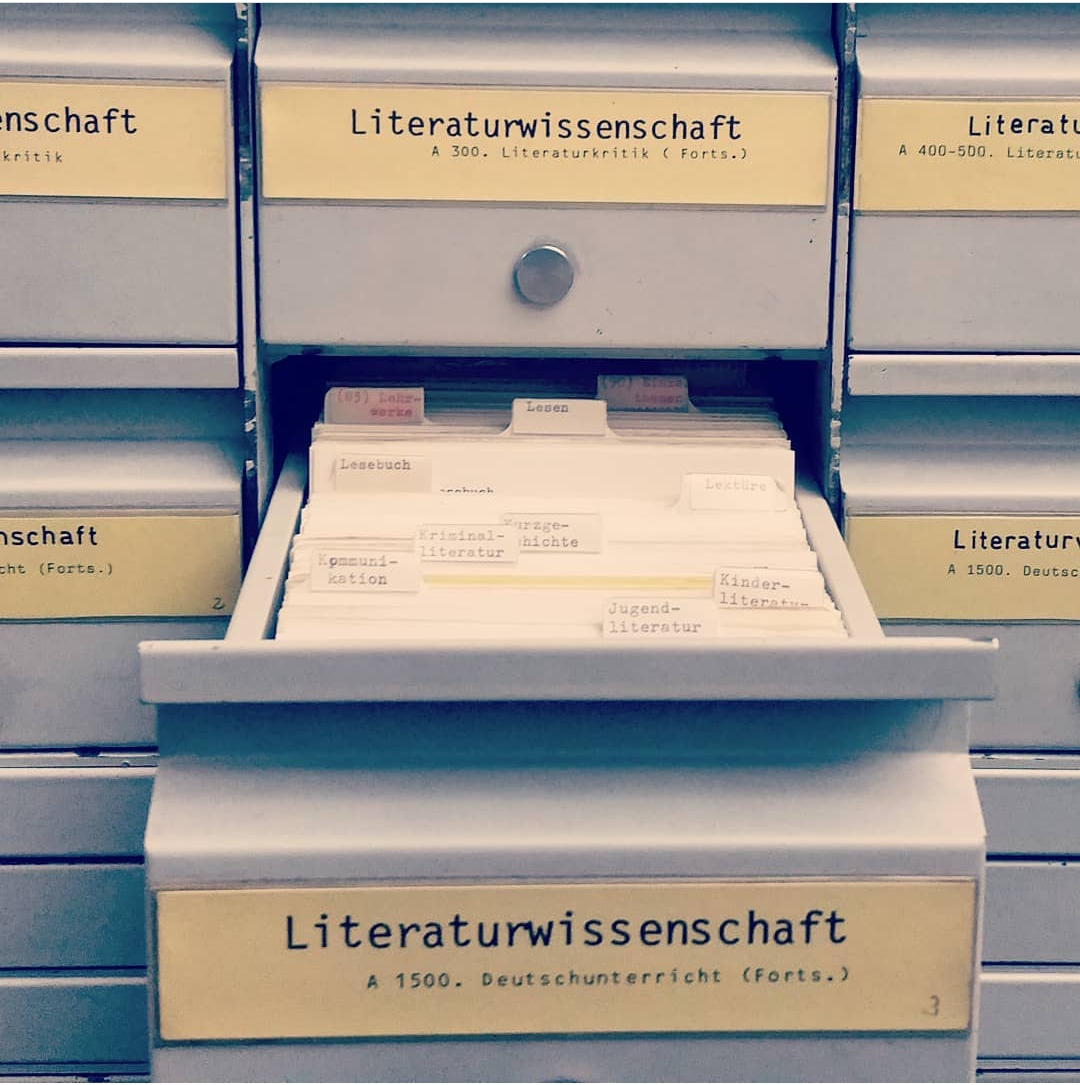
\includegraphics[keepaspectratio, width=\textwidth]{figures/Zettelkasten.jpg}
	\caption{Zettelkasten aus der \gls{jcs}. Quelle: {Petra Schneider}}
	\label{fig:zettelkasten}
\end{figure}
Die Zettelkästen wurden an der \gls{jcs},
wie auch an vielen anderen Bibliotheken,
durch einen \gls{opac} ersetzt,
der den Zugriff auf die Übersicht von überall bietet.
Als zusätzlicher Vorteil kommt bei digitalen Lösungen
die einfachere Suche über verschiedene Felder eines Eintrags hinzu.

Eine manuelle Sacherschließung hängt von den Fähigkeiten der erfassenden Person ab.
Somit ist,
trotz bibliothekarischer Regelwerke,
nicht sichergestellt,
dass alle relevanten Schlagworte und Themenkomplexe verzeichnet werden.
Die vollständige Verschlagwortung und Verknüpfung mit zusätzlichem Wissen
ist der Schritt Richtung \enquote{Semantic Web}
und Zukunft der Bibliotheken.
Durch solche Verknüpfungen wird die Information für die Nutzer noch besser zugänglich,
denn vom Eintrag sind die Themenbereiche zu erreichen,
welche auf alle Einträge verweisen.
Dies vereinfacht die Suche.

Im Rahmen dieser Aufgabe betreut die \gls{jcs}
mehrere \glspl{fachinformationsdienst}
mit finanzieller Förderung der \gls{dfg}
über deren Förderprogramm \enquote{Fachinformationsdienste für die Wissenschaft}
\footnote{\url{https://www.dfg.de/foerderung/programme/infrastruktur/lis/lis_foerderangebote/fachinfodienste_wissenschaft/index.html}}.
Diese sind in \cref{fig:fid:overview} dargestellt.

\begin{table}
	\begin{tabularx}{\textwidth}{l r}
		Afrikastudien                                      & \multirow{2}{*}{\href{http://www.ilissafrica.de/}{
\includegraphics[height=1cm]{figures/ilissLogo.png}}}            \\ \footnotesize{\url{http://www.ilissafrica.de/}} &\\[2ex]
		Allgemeine und Vergleichende Literaturwissenschaft & \multirow{2}{*}{\href{http://avldigital.de/}{
\includegraphics[height=1cm]{figures/avl.png}}}                       \\ \footnotesize{\url{http://avldigital.de/}}&\\[2ex]
		Biodiversitätsforschung                            & \multirow{2}{*}{\href{https://www.biofid.de/de/}{
\includegraphics[height=1cm]{figures/biofid_160.png}}}            \\ \footnotesize{\url{https://www.biofid.de/de/}} & \\[2ex]
		Darstellende Kunst                                 & \multirow{2}{*}{\href{http://www.performing-arts.eu/}{
\includegraphics[height=1cm]{figures/fid-dk_160.png}}}       \\ \footnotesize{\url{http://www.performing-arts.eu/}} & \\[2ex]
		Germanistik                                        & \multirow{2}{*}{\href{https://www.germanistik-im-netz.de/}{
\includegraphics[height=1cm]{figures/gin_logo150.png}}} \\ \footnotesize{\url{https://www.germanistik-im-netz.de/}} & \\[2ex]
		Jüdische Studien                                   & \multirow{2}{*}{\href{https://www.jewishstudies.de/}{
\includegraphics[height=1cm]{figures/fid-js_160.png}}}        \\ \footnotesize{\url{https://www.jewishstudies.de/}} & \\[2ex]
		Linguistik                                         & \multirow{2}{*}{\href{http://www.linguistik.de/}{
\includegraphics[height=1cm]{figures/linguistik_160.png}}}        \\ \footnotesize{\url{http://www.linguistik.de}} &
	\end{tabularx}
	\caption{Übersicht der \glspl{fachinformationsdienst} der \gls{jcs} \autocite{ub:sammlungen:fid}}
	\label{fig:fid:overview}
\end{table}

Der \gls{fachinformationsdienst} Linguistik ist
\textquote[\autocite{ub:projekte:fid-linguistik}]{ein Kooperationsprojekt zwischen der Universitätsbibliothek Johann Christian Senckenberg und  Prof. Christian Chiarcos vom Forschungsgebiet Angewandte Computerlinguistik (AcoLi) am Institut für Informatik der Goethe Universität}
und betreibt das Lin|gu|is|tik-Portal,
welches im folgenden Abschnitt beschrieben wird.

\subsection{Das Portal}
\blockquote[\autocite{ub:projekte:fid-linguistik}]{Das Lin|gu|is|tik-Portal ist
	ein Fachportal für die allgemeine und vergleichende Sprachwissenschaft
	sowie die Linguistiken der europäischen und außereuropäischen Einzelphilologien.}
Es weist
die Titelmetadaten,
wie z.B.\, den Autor, den Titel oder das Thema,
verschiedener Publikationen nach.
Um den Nutzen für die Forschung zu steigern,
soll in Zukunft eine Volltextsuche über die \gls{openaccess}[-Texte]
hinzugefügt werden.
Diese soll durch einen Index auf Basis von \glspl{knowledgebase},
wie z.B.\, der \gls{bllontology}, WikiData oder GND-Sachbegriffen
unterstützt werden,
indem die Volltexte mit semantischen Deskriptoren versehen werden.

\subsection{Die Ziele}
\label{ssec:ziele}
Das Ziel dieser Arbeit ist die Implementierung eines mehrschrittigen Prozesses.
Zuerst sollen \glsfirst{bll}[-Termini] in linguistischen Texten erkannt werden (\gls{namedentityrecognition}).
Diesen Schritt bezeichnet man teilweise als \gls{mentiondetection},
denn die meisten Prozesse erkennen hier noch keine Entitäten.
Stattdessen werden Kandidaten für Entitäten erkannt.
Nachdem diese Kandidaten erkannt sind,
werden im Schritt der \gls{namedentitydisambiguation}
die gefundenen Kandidaten mit der \gls{knowledgebase} abgeglichen.
Um diesen Abgleich effizienter zu machen,
wird oft für jede Mention eine Liste von möglichen Kanditation aus der \gls{knowledgebase} extrahiert
(English: \foreigntextquote{english}{Candidate Generation})\autocite{Raheim2022}
und der geeignetste Kanditat aus der \gls{knowledgebase} ausgewählt.
Dies ist insbesondere bei sehr breiten \glspl{knowledgebase} wichtig,
in denen Benennung von Entitäten mehrfach vorkommen;
so listet \citeauthor{dewiki:209960843}
für die Abkürzung \emph{FFM}\autocite{dewiki:209960843}
neben der Bedeutung \emph{Frankfurt am Main}\autocite{dewiki:225740004} noch 14 weitere Bedeutungen,
wie in \cref{tbl:ffm} zu sehen ist,
zwischen denen aus dem Kontext entschieden werden müsste.

\begin{table}
	\begin{tabularx}{\textwidth}{l l}
		Fachschule für Foto- und Medientechnik & Fixed Frequency Modem              \\
		Fast Food Musical                      & Frankfurt am Main                  \\
		Fédération française de motocyclisme   & Frankfurter Feldbahnmuseum         \\
		Fédération Française Motonautique      & Fudbalska Federacija na Makedonija \\
		Female Female Male                     & Fünf-Faktoren-Modell               \\
		Festival des Films du Monde            & Full Face Mask                     \\
		Fettfreie Masse                        & Fused Filament Fabrication         \\
		Firefly                                & Maasina-Fulfulde
	\end{tabularx}
	\caption{
		Übersicht der Bedeutungen der Abkürzung \emph{FFM}, bzw.\, \emph{ffm}
		nach \citetitle{dewiki:209960843} \autocite{dewiki:209960843}
	}
	\label{tbl:ffm}
\end{table}

Im letzten Schritt wird die Mention im Text mit dem ausgewählten Kanditaten aus der \gls{knowledgebase}
annotiert bzw.\, verknüpft \gls{namedentitylinking}.

Durch eine solche Verlinkung
können bei den Einträgen im Portal die Metadaten ergänzt werden
und somit die Suche nach Artikeln zu einem bestimmten Thema vereinfacht werden.
Es ist denkbar,
die annotierten Texte direkt darzustellen
und Nutzenden so ein \enquote{Nachschlagen}
von Begriffen in der \gls{bllontology} zu ermöglichen.

Im ersten Satz von \citetitle{dewiki:225740004} werden alleine sieben verschiedene weitere Wikipedia Entitäten und eine Wikimedia Entität verlinkt,
wie in \cref{tbl:wikipedia:Frankfurt_am_Main:linking} zu sehen ist.

\begin{table}
	\begin{adjustbox}{max width=0.8\linewidth,}
		\begin{tabularx}{\textwidth}{l l}
			Frankfurt am Main          &                                                                                               \\
			(                          &                                                                                               \\
			anhören                    & {\url{https://upload.wikimedia.org/wikipedia/commons/1/13/De-Frankfurt_a._M..ogg}}            \\
			\textsuperscript{?}        & {\url{https://de.wikipedia.org/wiki/Hilfe:Audio}}                                             \\
			\textsuperscript{/}        &                                                                                               \\
			\textsuperscript{i}        & {\url{https://de.wikipedia.org/wiki/Datei:De-Frankfurt_a._M..ogg}}                            \\
			)                          &                                                                                               \\
			ist mit 759.224            &                                                                                               \\
			Einwohnern                 & {\url{https://de.wikipedia.org/wiki/Einwohnerentwicklung_von_Frankfurt_am_Main}}              \\
			(31. Dezember 2021) die    &                                                                                               \\
			bevölkerungsreichste Stadt & {\url{https://de.wikipedia.org/wiki/Liste_der_gr\%C3\%B6\%C3\%9Ften_St\%C3\%A4dte_in_Hessen}} \\
			des Landes                 &                                                                                               \\
			Hessen                     & {\url{https://de.wikipedia.org/wiki/Hessen}}                                                  \\
			und die                    &                                                                                               \\
			fünftgrößte                & {\url{https://de.wikipedia.org/wiki/Liste_der_Gro\%C3\%9Fst\%C3\%A4dte_in_Deutschland}}       \\
			Deutschlands               & {\url{https://de.wikipedia.org/wiki/Deutschland}}                                             \\
			.                          &
		\end{tabularx}
	\end{adjustbox}
	\caption{Übersicht der Verlinkungen des ersten Satzes von \citetitle{dewiki:225740004}\autocite{dewiki:225740004}}
	\label{tbl:wikipedia:Frankfurt_am_Main:linking}
\end{table}

Solch eine Verknüpfung von Informationen
vereinfacht eine Auseinandersetzung mit den Inhalten
und ermöglicht Metaanalysen.

\subsection{Die Modelle}
\gls{BERT} ist ein state-of-the-art % CHECK \gls{stateoftheart}
Modell
für \gls{naturallanguageprocessing} Aufgaben.\autocite{1810.04805}
Es bietet sich somit für die in \Cref{ssec:ziele} beschriebene Aufgabe an.
Es wurde in \citetitle{1810.04805}
von \citeauthor{1810.04805}
vorgestellt und basiert auf der \gls{transformer}[ Architektur].\autocite{1810.04805}
\gls{BERT} gehört zu einer neuen Generation von \glslink{neuralnetwork}{neuronalen Netzen},
welche vortrainiert (English: \foreigntextquote{english}{pretrained}) sind.
Das bedeutet,
dass der aufwendige \gls{unsupervised-learning} Teil des Trainings
zwischen den verschiedenen Aufgaben geteilt wird.
Für neue Aufgaben muss nur das finale \gls{supervised-learning} durchgeführt werden,
damit das Modell auf die Aufgabe abgesimmt ist.
Auf Englisch bezeichnet man ein abgestimmtes Modell als \foreigntextquote{english}{fine-tuned}.
Das \gls{GBERT} Modell ist eine auf deutschsprachigen Daten trainierte Variante
dieser Architektur von \citeauthor{2010.10906}.
\autocite{2010.10906}
Die \gls{transformer}[ Architektur]
ist für \gls{naturallanguageprocessing} vorteilhaft,
weil sie beidseitigen Kontext für die Bewertung der Wörter nutzt.
\gls{GBERT} ist insbesondere geeignet,
da dieses Modell bereits auf Deutsch als Sprache optimiert ist.

Dank \gls{exBERT}
kann man manuell das Modell erkunden
und versuchen zu erkennen,
welche Zusammenhänge bereits im Modell enthalten sind.

Sei der Beispielsatz
\blockquote[\autocite{dewiki:225740004}]{Frankfurt am Main ( anhören?/i) ist mit 759.224 Einwohnern (31. Dezember 2021) die bevölkerungsreichste Stadt des Landes Hessen und die fünftgrößte Deutschlands}
wieder gegeben
und sei das betrachte Modell \texttt{bert-base-german-uncased}.
Der Fokus wird auf den Token \enquote{Frankfurt}, \enquote{Main} und \enquote{Hessen}
liegen.
Ohne Maskierung wird der Token jeweils mit einer Sicherheit von 1 prognostiziert.
Eine Maskierung eines einzelnen der drei Token führt nur bei \enquote{Hessen} dazu,
dass der Token als \texttt{[unused\_punctuation2]} (also als \enquote{-} nach \cref{lst:vocab:txt:diff})
vorhersagt werden würde\footnote{Eine Maskierung des Wortes \enquote{Frankfurt} führt jedoch mit einer Konfidenz von 0.02 dazu, % CHECK prognostiziert? 
	% CHECK Frankfurt und Offenbach emph statt enquote
	dass \enquote{Offenbach} als Token vorhergesagt wird}.
Damit ist erkennbar,
dass das \texttt{bert-base-german-uncased} bereits viele Informationen über Zusammenhänge erkennt.
Dies liegt aber auch daran,
dass dieses Modell unter anderem auf Wikipedia Daten trainiert wurde.

% CHECK break
\begin{longlisting}
	\begin{tcolorbox}[tlistingstyle,breakable]
		\inputminted[
			fontsize=\footnotesize,
		]{output}{listings/vocab.txt.diff}
	\end{tcolorbox}
	\caption{Änderungen im Vokabular des \texttt{bert-base-german-uncased} Tokenizers.
		Diff aus den beiden in \autocite{deepset-ai:FARM:issues:60} referenzierten \texttt{vocab.txt} Dateien.
		Links die Bezeichnungen wie sie ursprünglich verwendet wurden, rechts die aktuelle Darstellung der Token}
	\label{lst:vocab:txt:diff}
\end{longlisting}

% Reset glossary first use after introduction
\glsresetall\mglsresetall

\section{Grundlagen und Definitionen}
Im folgenden Abschnitt gibt es eine kurze Einführung zum Thema \enquote{\gls{machine-learning}}. % CHECK emph statt enquote
Danach werden die für diese Arbeit relevanten Problemstellungen formuliert,
bevor die Datenquellen beschrieben werden.
Nachdem die Datenquellen bekannt sind,
wird die Erstellung von Trainingsdaten beschrieben,
woraufhin kurz auf die Architektur von \gls{BERT} eingegangen wird.


\subsection{\Gls{machine-learning}}


\subsubsection{Bewertung \glslink{machine-learning}{maschinellen Lernens}}
Die folgenden Metriken werden oft genutzt,
um die Güte eines Modells darzustellen:
\gls{nlp:stats:loss},
\gls{nlp:stats:recall},
\gls{nlp:stats:precision} und
\gls{nlp:stats:f1}.

Zum besseren Verständnis werden im folgenden einige Begriffe eingeführt,
bevor diese Metriken definiert werden.
\begin{defn}[Typische Benennung bei binärer Kategorisierung]
	Data ist hierbei die \enquote{Wahrheit},
	während \enquote{Prediction} die Kategorisierung durch das System ist.
	\begin{center}
		\begin{tabularx}{0.8\textwidth}{l l | c c | r}
			                               &                   & \multicolumn{2}{c|}{\textbf{Prediction}} &                                      \\
			                               &                   & \textbf{Positive}                        & \textbf{Negative}  & $\sum$          \\
			\cline{1-5}
			\multirow{2}{*}{\textbf{Data}} & \textbf{Positive} & True Positive                            & False Negative     & Actual Positive \\
			                               & \textbf{Negative} & False Positive                           & True Negative      & Actual Negative \\
			\cline{1-5}
			                               & $\sum$            & Predicted Positive                       & Predicted Negative &
		\end{tabularx}
	\end{center}
	\captionof{table}{\gls{confusion-matrix}, welche die typischen Bezeichnungen der Merkmalsausprägungen für eine binäre Klassifikation zeigt}
\end{defn}
\FloatBarrier

Für die Nachvollziehbarkeit wird in \cref{tbl:exampledistribution} die \gls{confusion-matrix} mit beispielhaften Zahlen gefüllt.
% CHECK non floating
\begin{table}[H]
	\begin{center}
		\begin{tabularx}{0.5\textwidth}{l l | c c | r}
			                               &                   & \multicolumn{2}{c|}{\textbf{Prediction}} &                            \\
			                               &                   & \textbf{Positive}                        & \textbf{Negative} & $\sum$ \\
			\cline{1-5}
			\multirow{2}{*}{\textbf{Data}} & \textbf{Positive} & 5                                        & 5                 & 10     \\
			                               & \textbf{Negative} & 90                                       & 9900              & 9990   \\
			\cline{1-5}
			                               & $\sum$            & 95                                       & 9905              &
		\end{tabularx}
	\end{center}
	\caption{Beispielhafte Verteilung}
	\label{tbl:exampledistribution}
\end{table}

Die Formeln für diese sind nach \citeauthor{towardsdatascience:stats}
wie folgt \autocite{towardsdatascience:stats} definiert:

\begin{defn}[\glspt{nlp:stats:precision}]
	\begin{equation}
		\label{eqn:precision}
		\text{Precision}
		= \frac{\text{True Positive}}{\text{True Positive}+\text{False Positive}}
		= \frac{\text{True Positive}}{\text{Predicted Positive}}
	\end{equation}
\end{defn}

Somit wäre für \cref{tbl:exampledistribution}
die Precision
\(\frac{5}{95} \approx 5,3\% \).

\begin{defn}[\glspt{nlp:stats:recall}]
	\begin{equation}
		\label{eqn:recall}
		\text{Recall}
		= \frac{\text{True Positive}}{\text{True Positive}+\text{False Negative}}
		= \frac{\text{True Positive}}{\text{Actual Positive}}
	\end{equation}
\end{defn}

Für unser Beispiel \cref{tbl:exampledistribution}
ergibt sich ein Recall von \(\frac{5}{10} = 50\% \).

\begin{defn}[\glspt{nlp:stats:f1}]
	\begin{equation}
		\label{eqn:f1}
		\text{F1}
		= 2 \times \frac{\text{Precision}\times\text{Recall}}{\text{Precision}+\text{Recall}}
	\end{equation}
\end{defn}

Der F1-Wert ist also
\(2 \times \frac{\frac{5}{95}\times\frac{5}{10}}{\frac{5}{95}+\frac{5}{10}}=\frac{2}{21} \approx 9,5\%\).


\nocite{overleaf:HowToThesisPart3}
\begin{table}
	\begin{subtable}{0.45\textwidth}
		\begin{center}
			\begin{tabularx}{\textwidth}{l l | c c | r}
				                               &                   & \multicolumn{2}{c|}{\textbf{Prediction}} &                            \\
				                               &                   & \textbf{Positive}                        & \textbf{Negative} & $\sum$ \\
				\cline{1-5}
				\multirow{2}{*}{\textbf{Data}} & \textbf{Positive} & 10                                       & 0                 & 10     \\
				                               & \textbf{Negative} & 9990                                     & 0                 & 9990   \\
				\cline{1-5}
				                               & $\sum$            & 10 000                                   & 0                 &
			\end{tabularx}
		\end{center}

		\caption{Optimistisches Modell}
		\label{tbl:optimisticmodell}
	\end{subtable}
	\hfill
	\begin{subtable}{0.45\textwidth}
		\begin{center}
			\begin{tabularx}{\textwidth}{l l | c c | r}
				                               &                   & \multicolumn{2}{c|}{\textbf{Prediction}} &                            \\
				                               &                   & \textbf{Positive}                        & \textbf{Negative} & $\sum$ \\
				\cline{1-5}
				\multirow{2}{*}{\textbf{Data}} & \textbf{Positive} & 0                                        & 10                & 10     \\
				                               & \textbf{Negative} & 0                                        & 9990              & 9990   \\
				\cline{1-5}
				                               & $\sum$            & 0                                        & 10 000            &
			\end{tabularx}
		\end{center}
		\caption{Pessimistisches Modell}
		\label{tbl:pessimisticmodell}
	\end{subtable}
	\caption{Konstante Modelle}
	\label{tbl:constant-modells}
\end{table}

Sei ein Modell gegeben, 
welches immer positiv bzw. immer negativ vorhersagt,
dann sehen die Matritzen wie in \cref{tbl:optimisticmodell} bzw. in \cref{tbl:pessimisticmodell} aus.
Diese erhalten die Werte in \cref{tbl:examplemetricsoverview}.

\begin{table}
	\begin{center}
		\begin{tabularx}{0.5\textwidth}{l r r r}
			          & Optimistic & Pessimistic & Example   \\
			Precision & \(0,1\%\)  & NA          & \(5,3\%\) \\
			Recall    & \(100\%\)  & \(0\%\)     & \(50\%\)  \\
			F1        & \( 100\%\) & NA          & \(9.5\%\)
		\end{tabularx}
	\end{center}
	\caption{Tabellarischer Vergleich der Metriken an einem optimistischen, einem pessimistischen und dem ursprünglichen-Beispiel Modell}
	\label{tbl:examplemetricsoverview}
\end{table}

\begin{defn}[\glspt{nlp:stats:loss}\autocite{1906.01378}]
	Seien
	\(\mathbf{X} \in \mathcal{X}\)
	und
	\(Y \in \mathcal{Y}\)
	Zufallsvariablen,
	wobei
	\(\mathcal{X}\subset\mathbb{R}^d\)
	und
	\(\mathcal{Y} = \left\lbrace0,1\right\rbrace\).
	Eine \gls{nlp:stats:loss}[-Funktion]
	ist eine Abbildung
	\(\glssymbol{nlp:stats:loss}: \mathbb{R} \times \mathcal{Y} \to \mathbb{R}^{+}.\)
	Hierbei ist ein kleinerer Wert besser.
	\foreigntextquote{english}[\autocite{google:trainingandloss}]{Loss is the penalty for a bad prediction}
\end{defn}

Bei \gls{nlp:stats:loss} wird also nicht ein gutes Modell \enquote{belohnt},
sondern ein schlechtes Modell \enquote{bestraft}.
Für eine solche \gls{nlp:stats:loss}[ Funktion] \glssymbol{nlp:stats:loss}
lässt sich das \glssymbol{nlp:stats:loss}[-Risiko]
wie folgt definieren:

\begin{defn}[{\glssymbol{nlp:stats:loss}[-Risiko]\autocite{1906.01378}}]
	Seien
	\(\mathbf{X} \in \mathcal{X}\)
	und
	\(Y \in \mathcal{Y}\)
	Zufallsvariablen,
	wobei
	\(\mathcal{X}\subset\mathbb{R}^d\)
	und
	\(\mathcal{Y} = \left\lbrace0,1\right\rbrace\).
	Für eine beliebige \gls{nlp:stats:loss}[-Funktion] \glssymbol{nlp:stats:loss}
	und eine Klassifikationsfunktion \(f\),
	wird das \glssymbol{nlp:stats:loss}[-Risiko] definiert als:
	\begin{equation}
		\label{eqn:loss-risk}
		R_{\glssymbol{nlp:stats:loss}} \left(f\right)
		=
		\mathbb{E}_{\mathbf{X},Y} \glssymbol{nlp:stats:loss}\left(f(x) \mid y_{x}\right)
	\end{equation}
	wobei \(\mathbb{E}\) den Erwartungswert bezeichnet
	und der Index die Zufallsvariablen bezüglich derer er gebildet wird.
\end{defn}


\subsubsection{Arten \glslink{machine-learning}{maschinellen Lernens}}
\Gls{machine-learning} ist eine Unterkategorie von \gls{artificialintelligence}.
Das Ziel ist dem Computer die Möglichkeit zu geben zu lernen,
ohne explizit dafür programmiert zu sein \autocite{levity:howdomachineslearn}.

\citeauthor{levity:howdomachineslearn} unterteilt es in die drei folgenden großen Kategorien:


\begin{defn}[\gls{supervised-learning} \autocite{levity:howdomachineslearn}]
	\Gls{machine-learning}
	auf Basis von bereits annotierten Tupeln der Form
	\(\left(X, f(X)\right)\),
	wobei \(X\) eine Eingabe und \(f(X)\) die erwartete Ausgabe ist,
	nennt man \gls{supervised-learning}.
	Solche Tupel werden oft auch als \texttt{labeled data} bezeichnet.
\end{defn}

Hierbei sind nach \citeauthor{levity:howdomachineslearn}
die Hauptaufgaben Regression und Klassifikation.

Bei Klassifikation ist die Funktion definiert als
\(f: \mathcal{X} \to \mathcal{Y}  \),
wobei \(\mathcal{Y} = \left\lbrace \text{\texttt{LABEL}}_i \mid i=1 \vdots l \right\rbrace \)
die Menge der möglichen Klassen ist.
Der Wertebereich ist also diskret.\autocite{ledu:regression-versus-classification}
Bei Regression hingegen ist der Wertebereich kontinuierlich
und es gilt im Allgemeinen \(f: \mathcal{X} \to \mathbb{C}^{l}\)
bzw.\, \(f: \mathcal{X} \to \mathbb{R}^{l}\) .

Das so trainierte Modell ist ein Funktionsapproximation für \(f\).
Es gibt für eine Regressionsaufgabe eine Fortsetzung und Vereinfachung der bisherigen Funktion
und für Klassifikationsaufgaben Label für bisher unbekannte Eingaben.

Neuere Methoden reduzieren den Bedarf an Trainingsdaten,
indem sie diese nach bestimmten Regeln erzeugen.
Dies kann durch Einbindung externer Systeme geschehen,
wie z.B.\, bei \gls{distant-supervision} und \gls{reinforcement-learning}
oder nur auf Grundlage der Daten.

\begin{defn}[\gls{distant-supervision}\autocite{deepdive:stanford:distant-supervision}]
	Unter Verwendung einer bestehenden \gls{knowledgebase}
	wird die Eingabe mit einer erwarteten Ausgabe kombiniert,
	um \texttt{labeled data} für \gls{supervised-learning} zu erzeugen.
\end{defn}

\begin{defn}[\gls{reinforcement-learning} \autocite{levity:howdomachineslearn}]
	Hierbei gibt im Gegensatz zu \gls{supervised-learning} keine Tupel,
	sondern eine bewertende Instanz,
	die mitteilt,
	ob eine bestimmte Aktion oder Entscheidung des Modells
	\enquote{gut} oder \enquote{schlecht} war.
\end{defn}

\begin{defn}[\gls{unsupervised-learning} \autocite{levity:howdomachineslearn}]
	Beim \gls{unsupervised-learning} sind die Daten nicht weiter klassifiziert.
	Die Tupel \(\left(X, f(X)\right)\) können also nur automatisch erzeugt werden.
	Diese Art des Lernens nennt man auch \textquote[\autocite{ng:deeplearning}]{self-taught learning}.
\end{defn}

\label{ssec:dartstellbarkeit}
Da die Modelle meist durch Tensorberechnungen abgebildet werden,
ist eine Darstellung der Informationen als dünnbesetzter Vektor
von Vorteil.
So müssen weniger einzelne Berechnungen durchgeführt werden
und gleichzeitig sinkt durch eine solche Darstellung der Speicherbedarf.\autocite{10.1007/bf02331346}
Die Darstellbarkeit von Informationen als dünnbesetzte Vektoren 
in einer entsprechenden Basis wurde von \citeauthor{olshausen1996emergence}
bereits \citeyear{olshausen1996emergence} in \citetitle{olshausen1996emergence}
gezeigt. \autocite{olshausen1996emergence}
Solch eine Darstellung kann ein System
durch Optimierung nach einer \gls{nlp:stats:loss}[-Funktion],
die Informationserhaltung und Dünnbesetztheit betrachtet,
im Rahmen des \gls{unsupervised-learning}
einfach lernen. \autocite[Formel 2-4]{olshausen1996emergence}
% CHECK Add examples here


\subsection{\glsfmtfull{naturallanguageprocessing}}
Bei \gls{naturallanguageprocessing}
geht es um die Verarbeitung und Interpretation von menschlicher Sprache.
Das Ziel ist es Informationen zu gewinnen.

\subsubsection{\glsfmtfull{namedentityrecognition}}
Der Prozess der \gls{namedentityrecognition}
lässt sich nach \autocite{2006.15509} als Lösung des folgenden mathematischen Problems beschreiben:

\begin{prob}[\glsfmtfull{namedentityrecognition}]\label{prob:nlp:ner}
	Für einen \gls{nlp:sentence} \glsentryformula{nlp:sentence}
	wird eine \gls{nlp:label_sequence} \glsentryformula{nlp:label_sequence} gesucht.
	Die \texttt{BIO}-Klassifikation von \citeauthor{10.1145/2396761.2398506}
	\autocite{10.1145/2396761.2398506}
	fordert hierbei,
	dass \(
	\glssymbol{nlp:label}_i \in
	\left\lbrace
	\glssymbol{nlp:label:beginning}\texttt{-X},
	\glssymbol{nlp:label:inside}\texttt{-X},
	\glssymbol{nlp:label:outside}
	:
	\text{\texttt{X} ist Entitätstyp}
	\right\rbrace
	\)
	und dass gilt:
	\[
		\glssymbol{nlp:label}_i =
		\begin{cases}
			\texttt{\glssymbol{nlp:label:beginning}-X},
			\text{wenn \(\glssymbol{nlp:token}_i\)
				der Beginn einer Entität vom Typ \(\texttt{X}\) ist
			} \\
			\texttt{\glssymbol{nlp:label:inside}-X},
			\text{wenn \(\glssymbol{nlp:token}_i\)
				ein Token einer Entität vom Typ \(\texttt{X}\)
				und nicht deren Beginn ist
			} \\
			\glssymbol{nlp:label:outside}, \text{sonst}.
		\end{cases}
	\]
	Da die \glspl{nlp:sentence} meistens in Tokens aufgeteilt werden,
	spricht man auch von einer Tokenklassifizierung-Aufgabe.
\end{prob}

Der klassische Ansatz zur Erzeugung einer \gls{nlp:label_sequence} ist es,
die Eingabe in mehreren Schritten die Eingabe um Informationen (Features) anzureichern.
Diese werden in den jeweils darauf folgenden Schritten, unterstützend eingesetzt.
Dazu gehören z.B.\, \textquote[{\autocite[§19]{fortext-2018-id-36}}]{häufig vorher genannte Wörter (sowie z.B. bei Orten das Wort „in"),
	Darstellungsformat (bei Daten so etwas wie Zahl Monat Jahr),
	Groß- und Kleinschreibung} oder auch
die \textquote[{\autocite[§19]{fortext-2018-id-36}}]{Position im Satz}. % CHECK how this looks
Eine Darstellung einer beispielhaften \gls{naturallanguageprocessing}[-Architektur] ist in \Cref{fig:corenlp:architecture}
zu sehen.

% https://tex.stackexchange.com/questions/83069/how-to-stack-two-subfigures-next-to-a-third-subfigure
\nocite{stack:tex:two-subfigures-next-to-a-third-subfigure}
\begin{figure}
	\begin{subfigure}[b]{0.45\textwidth}
		\begin{tcolorbox}[tpipelinestyle]
			\begin{adjustbox}{center,max width=0.9\linewidth,max totalheight=0.9\textheight}
				\InputIfExists{figures/pipeline:corenlp.latex}
			\end{adjustbox}
		\end{tcolorbox}
		\caption{Darstellung der Architektur von Stanford CoreNLP \autocite[Figure 1]{P14-5010}}
		\label{fig:corenlp:architecture}
	\end{subfigure}
	\hfill
	\begin{subfigure}[b]{0.45\textwidth}
		\begin{tcolorbox}[tpipelinestyle]
			\begin{adjustbox}{center,max width=\linewidth,max totalheight=0.9\textheight}
				\InputIfExists{figures/pipeline:nlp:machinelearning.latex}
			\end{adjustbox}
		\end{tcolorbox}
		\caption{Aufbau der Pipeline für die Datenverarbeitung}
		\label{fig:pipeline:nlp:machinelearning}
		%\end{subfigure}

		\vfill

		%\begin{subfigure}[b]{0.45\textwidth}
		\begin{tcolorbox}[tpipelinestyle]
			\begin{adjustbox}{center,max width=\linewidth,max totalheight=0.9\textheight}
				\InputIfExists{figures/huggingface:model.latex}
			\end{adjustbox}
		\end{tcolorbox}
		\caption[Aufbau eines {\gls{transformer}[ Modells]}]{Aufbau eines \gls{transformer}[ Modells]:
			Der Tokenizer übersetzt die Eingabe in dünnbesetzte Vektoren über einer entsprechenden Basis.
			Diese Vektoren bzw.\, Tensoren werden dann durch den eigentlichen \gls{transformer}
			in eine kontextuelle Einbettung
			überführt.
			Diese wird dann durch den Head auf eine aufgabenspezifische Vorhersage umgerechnet.
		}
		\label{fig:huggingface:transformer}
	\end{subfigure}
	\caption{Darstellung von Architekturen und Pipelines}
\end{figure}

Ein gängiger Aufbau für eine \gls{naturallanguageprocessing}
Pipeline
auf Basis von \glslink{machine-learning}{maschinellem Lernen}
ist nach
\autocite{1910.03771}
der in \Cref{fig:pipeline:nlp:machinelearning} dargestellte.
Hierbei werden keine weiteren Features definiert
und das System muss diese selber erkennen.
\citeauthor{1905.05950} stellen in \citetitle{1905.05950} jedoch fest,
dass auch \gls{BERT} teilweise ähnliche Zwischenschritte
wie in der klassischen \gls{naturallanguageprocessing}[-Pipeline]
abbildet.\autocite{1905.05950}

In der Regel besteht ein solches \gls{naturallanguageprocessing}[-Modell] aus drei Stufen,
wie in \Cref{fig:huggingface:transformer} dargestellt ist.
Der Tokenizer wandelt den Text in eine numerische Repräsentation um.
Diese wird durch den \gls{transformer} in einen Tensor aus Wahrscheinlichkeiten umgerechnet.
Der head erstellt aus diesem Wahrscheinlichkeitstensor eine Interpretation für die Aufgabe.


Auf der Ebene des Tokenizers gibt es Unterschiede.
In \autocite[Table 1]{1910.11470} sind diese einfach zu erkennen,


\begin{figure}[ht]
	% https://latexdraw.com/draw-trees-in-tikz/
	\nocite{latexdraw:trees}
	\begin{tcolorbox}[tfigurestyle]
		\begin{center}
			\begin{tikzpicture}
	[
%		level 0/.style = {red!40!black},
%		level 1/.style = {orange!40!black},
%		level 2/.style = {yellow!40!black},
%		level 3/.style = {green!40!black},
%		level 4/.style = {cyan!40!black},
%		level 5/.style = {purple!40!black},
%		level1/.style = {red!40!black},
%		level2/.style = {orange!40!black},
%		level3/.style = {fill=yellow,draw=yellow!40!black},
%		level4/.style = {green!40!black},
%		level5/.style = {cyan!40!black},
%		level6/.style = {purple!40!black},
		level1/.style = {fill=red},
		level2/.style = {fill=orange},
		level3/.style = {fill=yellow},
		level4/.style = {fill=green},
		level5/.style = {fill=cyan},
		level6/.style = {fill=violet!70!white},
		every node/.append style = {draw, anchor = west},
		grow via three points={one child at (0.5,-0.8) and two children at (0.5,-0.8) and (0.5,-1.6)},
		edge from parent path={(\tikzparentnode\tikzparentanchor) |- (\tikzchildnode\tikzchildanchor)}]
	 
	
	\node[level1] {\gls{machine-learning}}
		child {
			node[level1] {Feature-engineered}
			}
		child {
			node[level2] {Feature-inferring}
			child {
				node[] {word}
			}
			child {
				node[] {character}
			}
			child {
				node[] {word+character}
			}
			child {
				node[] {word+character+affix}
			}
			}
		;
	\end{tikzpicture}
		\end{center}
	\end{tcolorbox}
	\caption[%
        Übersicht der Systemtypen für \glspt{machine-learning}%
    ]{
		Übersicht der Systemtypen für \gls{machine-learning} im Bereich \gls{naturallanguageprocessing}
		nach \autocite[Table 1]{1910.11470}\\
        Bei Feature-engineered Systemen werden die Features durch Menschen definiert,
        während Feature-inferring Systeme diese selbstständig aus den Trainingsdaten generieren.
	}%
	\label{fig:model:types}
\end{figure}


\begin{defn}[Güte eines Modells]
	Seien \(M\) bereits annotierte \glslink{nlp:sentence}{Sätze}
	\glsentryformula{nlp:labelled_sentences} gegeben
	und beschreibe \glsentryformula{nlp:model} ein \gls{namedentityrecognition}[-Modell],
	wobei \glssymbol{nlp:sentence} ein Satz
	und \glssymbol{nlp:model:parameters} die Parameter des Modells sind.
	Dann lässt sich anhand von \Cref{prob:nlp:ner}
	die Güte des Modells über eine Metrik bestimmen.
\end{defn}

Eine beliebte Metrik im Rahmen des \gls{machine-learning} ist die \gls{crossentropyloss}[-Funktion],
wie sie in \autocite[Abschnitt 5.5]{jurafsky2000speech} definiert wird:
\glsentryformula{crossentropyloss}.
Hierbei wäre der ideale Fall,
dass jeder Satz
\glspl{nlp:label} entsprechend der vorgegeben (idealen) Annotation
zugewiesen bekommt.

\begin{thm}
	Dementsprechend werden die \gls{nlp:model:parameters} so gesucht,
	dass sie diese Distanz über alle Trainingsdaten minimieren.
	Somit sind die idealen Parameter für die \(M\) \glslink{nlp:sentence}{Sätze}
	durch die Formel
	\autocite[1]{2006.15509}
	gegeben:
	\begin{equation}
		\hat{\glssymbol{nlp:model:parameters}} : =
		\argmin_{\glssymbol{nlp:model:parameters}}
		\frac{1}{M}
		\sum_{m=1}^{M}
		\glssymbol{crossentropyloss}\left(
		\glssymbol{nlp:label_sequence}_m,
		\glssymbol{nlp:model}\left(
			\glssymbol{nlp:sentence}_m;
			\glssymbol{nlp:model:parameters}
			\right)
		\right)
	\end{equation}
\end{thm}

\subsubsection{\glsfmtfull{namedentitylinking}}
Das Ziel von \gls{namedentitylinking} ist es
die die per \gls{namedentityrecognition} erkannten Entitäten
mit einer \gls{knowledgebase} zuverknüpfen.
Dies lässt sich als folgendes Problem darstellen.

\begin{prob}[\glsfmtfull{namedentitylinking}]\label{prob:nlp:nel}
	Für einen \gls{nlp:sentence} \glsentryformula{nlp:sentence}
	wird eine \gls{nlp:label_sequence} \glsentryformula{nlp:label_sequence} gesucht,
	sodass \(
	\glssymbol{nlp:label}_i \in
	\left\lbrace
	\text{Entitätsreferenz}
	\right\rbrace
	\cup
	\left\lbrace
	\text{NONE}
	\right\rbrace
	\).
\end{prob}

Da es oftmals mehrere Kandidaten  für die Verlinkung in der \gls{knowledgebase} gibt,
wird im Schritt der \gls{namedentitydisambiguation} eine ausgewählt.

\subsection{Datenquellen}
Im Folgenden werden die zwei Datenquellen,
die für diese Arbeit verwendet wurden,
beschrieben.
Die erste Datenquelle ist die \gls{bllontology},
die für die Erstellung der Annotationen benötigt wird.
Danach folgt das \glsfmtfull{oai-pmh},
welches die zu annotierenden Daten liefert.

\subsubsection{\glspt{bllontology}}


\begin{defn}[Thesaurus\autocite{Arano:ThesaurusAndOntologies}] 
	Ein Thesaurus 
	ist eine Art von dokumentierender
	Sprache,
	die die konzeptuelle Struktur des Wissens eines bestimmten Fachgebietes
	darstellt.
	Er stellt den semantischen Zusammenhang zwischen verschieden Konzepten
	durch ein eingeschränktes Vokabular für die Beziehungen
	dar.
\end{defn}

Das Ziel eines Thesaurus ist \enquote{synonymy},
also die Überlappung der Bedeutung von Wörtern \autocite{oxfordbibliographies:Synonymy},
und \enquote{polysemy},
also die Mehrdeutigkeit der Bedeutung innerhalb eines Bereiches \autocite{oxfordbibliographies:Polysemy},
zu reduzieren.

Im Folgenden werden Beispiele von Dateien in der \gls{turtle}[ Syntax] gezeigt \autocite{w3c:turtle}.
Diese wird daher kurz erklärt.

Die Syntax besteht im Grunde nur aus Tripeln von \emph{Subjekt}, \emph{Prädikat} und \emph{Objekt}.
Zur Vereinfachung bleibt das aktuelle \emph{Subjekt} bis zum nächsten \emph{Punkt (.)}
und das aktuelle \emph{Prädikat} bis zum nächsten \emph{Semikolon (;)} aktiv.
Ein \emph{Komma (,)} trennt in diesem Zusammenhang die \emph{Objekte}.
Bei StringLiterals 
ist eine \gls{i18n}
möglich.
\mintinline{turtle}{"TEXT"@de} ist somit als String für die Sprache Deutsch definiert.

Damit die Konzepte eineindeutig sind,
werden sie über \gls{uri} beschrieben;
zur Vereinfachung können diese aber durch global erklärte Präfixe ersetzt werden.
Ein Beispiel hierfür ist in \Cref{lst:bll:thesaurus:prefixes}.

\begin{listing}
	\begin{tcolorbox}[tlistingstyle]
		\inputminted[
			firstline=1,
			lastline=13
		]{turtle}{../data/bll-thesaurus.ttl}
	\end{tcolorbox}
	\caption{Erklärung der globalen Präfixe in der \texttt{bll-thesaurus.ttl}}
	\label{lst:bll:thesaurus:prefixes}
\end{listing}

Nach dem die Präfixe
erklärt sind,
sind die zwei beispielhaften Einträge in \Cref{lst:bll:thesaurus:seneca} eindeutig definiert.
Der Eintrag \mintinline{turtle}{bllt:bll-133103862}
ist eine Klasse und ein Konzept.
Er wird durch \mintinline{turtle}{"Seneca"}
sowohl auf Deutsch,
als auch auf Englisch
und sowohl für das Konzept,
wie auch für die Anzeige klassifiziert.
Er ist eine Unterklasse von \mintinline{turtle}{bllt:BLLConcept}.
Als gröbere Klassifizierung gilt \mintinline{turtle}{bllt:bll-133108791} (Irokesisch).
Die Notation \mintinline{turtle}{"02.25.01.047.06"} repräsentiert diese Hierarchie,
wie in \Cref{fig:bll:notation:seneca}
zu sehen ist.

\begin{listing}[ht]
	\begin{tcolorbox}[tlistingstyle]
		\inputminted[
			firstline=12171,
			lastline=12183
		]{turtle}{../data/bll-thesaurus.ttl}
	\end{tcolorbox}
	\caption{Beispieleinträge aus \texttt{bll-thesaurus.ttl}}
	\label{lst:bll:thesaurus:seneca}
\end{listing}

\begin{figure}[ht]
	% https://latexdraw.com/draw-trees-in-tikz/
	\nocite{latexdraw:trees}
	\begin{tcolorbox}[tfigurestyle]
		\begin{center}
			\begin{tikzpicture}
	[
		level1/.style = {fill=red},
		level2/.style = {fill=orange},
		level3/.style = {fill=yellow},
		level4/.style = {fill=green},
		level5/.style = {fill=cyan},
		level6/.style = {fill=violet!70!white},
		every node/.append style = {draw, anchor = west},
		grow via three points={one child at (0.5,-0.8) and two children at (0.5,-0.8) and (0.5,-1.6)},
		edge from parent path={(\tikzparentnode\tikzparentanchor) |- (\tikzchildnode\tikzchildanchor)}]
	 
	
	\node[level1] {00}
		child {node[level1] {BLL-Klassifikation} edge from parent [dashed]}
		child {
			node[level2] {02}
			child {node[level2] {Nicht-indoeuropäische Sprachen} edge from parent [dashed]}
			child {
				node[level3] {02.25}
				child {node[level3] {Indigene amerikanische Sprachen} edge from parent [dashed]}
				child {
					node[level4] {02.25.01}
					child {node[level4] {Indigene Sprachen Nordamerikas und Zentralamerikas} edge from parent [dashed]}
					child {
						node[level5] {02.25.01.047}
						child {node[level5] {Irokesisch} edge from parent [dashed]}
						child {
							node[level6] {02.25.01.047.06 }
							child {node[level6] {Seneca} edge from parent [dashed]}
						}
					}
				}
			}
		};
	\end{tikzpicture}
		\end{center}
	\end{tcolorbox}
	\caption{Darstellung der Notation des Eintrages \Cref{lst:bll:thesaurus:seneca} als Baum mit den übergeordneten Klassen}%
	\label{fig:bll:notation:seneca}
\end{figure}

\FloatBarrier
\begin{defn}[\glspt{ontology}\autocite{10.1016/S0169-023X:97:00056-6}\autocite{Arano:ThesaurusAndOntologies}]
	\foreignblockquote{english}[{\autocite[Abschnitt 1.]{10.1006/knac.1993.1008}  und \autocite[Abschnitt 2.1]{Borst1997} via \autocite[Abschnitt 6.1]{10.1016/S0169-023X:97:00056-6}} ]{An ontology is a formal, explicit specification of a shared conceptualisation}
	wobei die folgenden Definitionen gelten:

	\begin{enumerate}
		\item Konzeptualisierung
		      : Ein abstraktes Modell eines Phänomens der realen Welt basierend auf den relevanten Konzepten des Phänomens
		\item Explizit: der Typ des Konzepts und die Einschränkungen seiner Nutzing sind explizit definiert
		\item Formal: Die Syntax ist präzise genug, um von einem Computer verstanden zu werden
		\item Geteilt: das Wissen ist von einer Gruppe akzeptiert
	\end{enumerate}

	Die Konzeptualisierung
	wird von \citeauthor{Arano:ThesaurusAndOntologies}
	noch weiter spezifiert,
	sodass sie eine Perspektive eine bestimmten Realität involvieren muss
	und diese auf der konzeptuellen Struktur einer \gls{knowledgebase}
	begründet wird.

	Das Ziel einer \gls{ontology}
	ist das Teilen des Wissens,
	welches sie repräsentiert.
\end{defn}
\FloatBarrier

Da sich die Präfixe in der \gls{ontology}
von denen im Thesaurus 
unterscheiden,
werden sie in \Cref{lst:bll:ontoloy:prefixes} noch einmal explizit dargestellt.

\begin{listing}
	\begin{tcolorbox}[tlistingstyle]
		\inputminted[
			firstline=1,
			lastline=6
		]{turtle}{listings/turtle:shortened:bll-ontology.ttl}
	\end{tcolorbox}
	\caption{Erklärung der globalen Präfixe in der \texttt{bll-ontology.ttl}}
	\label{lst:bll:ontoloy:prefixes}
\end{listing}

Nachdem die Präfixe
erklärt sind,
sind die zwei beispielhaften Einträge in \Cref{lst:bll:ontology:seneca} eindeutig definiert.
Das erste Beispiel ist wieder \mintinline{turtle}{"Seneca"}.
Dieses Mal ist die Klassifizierung als \enquote{\mintinline{turtle}{a skos:Concept}} % CHECK linebreak
nicht mehr enthalten,
dafür ist die neue Klassifikation 
als \enquote{\mintinline{turtle}{rdfs:subClassOf bllt:NorthernIroquoian}} % CHECK format
hinzugekommenen.
Das Format dieser \enquote{Elternklasse} zeigt an,
dass es eine manuell angelegte Klasse ist,
da der Name innerhalb des \texttt{bllt}-Namespaces keine Nummer ist.
Das zweite Beispiel zeigt zusätzliche Prädikate in der \gls{owl}[-Syntax],
wie Versionierungsinformationen und Äquivalenz.

\begin{listing}
	\begin{tcolorbox}[tlistingstyle]
		\inputminted[
			firstline=8,
			lastline=25
		]{turtle}{listings/turtle:shortened:bll-ontology.ttl}
	\end{tcolorbox}
	\caption{Leicht umformatierte Beispieleinträge aus \texttt{bll-ontology.ttl}
		(Der Zeilenumbruch nach dem Subjekt ist jeweils entfernt,
		damit das Syntaxhighlighting mit \gls{pygments} funktioniert)
	}
	\label{lst:bll:ontology:seneca}
\end{listing}


\begin{defn}[\glsfmtfull{bll}]
	Die \gls{bll} ist eine Bibliographie,
	also ein Verzeichnis von Literaturnachweisen
	zu linguistischer Literatur,
	insbesondere der Allgemeinen Linguistik
	und \textquote[\autocite{linguistik:de:kataloge:info}]{der anglistischen, germanistischen und romanistischen Sprachwissenschaft}.
\end{defn}

Zu dem oben genannten Verzeichnis existiert der \gls{bll}[ Thesaurus],
welcher für die Indizierung im Portal verwendet wird.
Bei der Umwandelung des \gls{bll}[ Thesaurus] in die \gls{bllontology},
die initial von \citeauthor{L16-1707} durchgeführt wird \autocite{L16-1707},
wird der Umfang an Begriffen eingeschränkt
auf Konzepte aus den Zweigen \foreigntextquote{english}[\autocite{data:linguistic:ontology-doc}]{Syntax, Morphology, Lexicology and Phonology}
und einigen zusätzlichen Einträgen aus den Zweigen \foreigntextquote{english}[\autocite{data:linguistic:ontology-doc}]{Graphemics and Semantics}.
Daher ist z.B.\,  der Term \texttt{bllt:bll-467296421} aus \Cref{lst:bll:thesaurus:seneca}
nicht in der \gls{bllontology} verzeichnet.

\subsubsection{\glsfmtfull{oai-pmh}}
Die \glsfmtfull{openarchivesinitiative} hat mit \gls{oai-pmh}
einen Standard für Interoperabilität zwischen verschiedenen Metadaten-Quellen
und Dienstanbietern definiert.
In \Cref{lst:oaipmh:xml:begin} ist der Anfang einer mit \gls{oaipmharvest} erzeugten
\gls{xml}[-Datei] dargestellt.

\begin{longlisting}
	\begin{tcolorbox}[tlistingstyle]
		\inputminted[
			firstline=1,
			lastline=21,
			fontsize=\footnotesize,
			escapeinside=||,
			gobble=10
		]{xml}{listings/oaixml:shortened:2022-07-13__oai_dc__000000000000.xml}
	\end{tcolorbox}
	\nopagebreak
	\caption{Beispiel Beginn eines \gls{oai-pmh}[-Eintrags]}
	\label{lst:oaipmh:xml:begin}
\end{longlisting}

Da der Inhalt innerhalb des \mintinline{xml}{oai_dc:dc}-Tags
durch das \gls{dublin-core}\footnote{\url{https://www.dublincore.org/specifications/dublin-core/dces/1999-07-02/}}
festgelegt ist,
liegt hier der Fokus.
Durch den Standard sind
der Titel (\mintinline{xml}{dc:title}),
das Thema (\mintinline{xml}{dc:subject}), welches oft als Liste von Schlagworten ausgedrückt wird,
Beschreibungen (\mintinline{xml}{dc:description})
und
eindeutige Referenzen (\mintinline{xml}{dc:identifier}) auf die Ressource
als Einträge definiert.
Auch die verwandten Ressourcen (\mintinline{xml}{dc:relation})
und das Format (\mintinline{xml}{dc:format})
sind enthalten.

Wenn der Volltext benötigt wird,
müssen die \mintinline{xml}{dc:identifier} oder die \mintinline{xml}{dc:relation}-Einträge
betrachtet werden.
Je nach Anbieter können hier bereits Referenzen auf Volltext-Dokumente hinterlegt sein
oder die Referenzen weisen nur auf Webseiten,
auf welchen die Referenzen auf die Volltext-Dokumente gefunden werden müssen.


Sowohl für \Cref{prob:nlp:ner} als auch für \Cref{prob:nlp:nel}
werden annotierte Daten benötigt.

\subsection{Erstellung von Trainingsdaten}
Da Trainingsdaten annotierte Daten sind,
wird nachfolgend auf die Arten und die Erstellung von Annotationen eingegangen.

\subsubsection{Arten der Annotation}

Eine mögliche Annotation ist es, 
den Wörtern eines Satzes ihre grammatikalische Funktion
oder andere semantische Informationen
zuzuordnen.
Wenn die semantische Information ist,
dass die annotierte Entität eine \enquote{spezielle} Entität ist,
welche einen Namen hat,
dann spricht man von \gls{namedentityrecognition}.
Auch eine Annotation über die Referenz auf die Entität ist möglich.

Da es keine bestehenden Annotationen für die Daten gibt,
sollen hier Möglichkeiten für die automatische Erzeugung betrachtet werden.

\subsubsection{Automatische Erzeugung von Annotationen}

\citeauthor{2006.15509} listet als Möglichkeiten für die automatische Annotation
\enquote{Stringmatchingg}, \enquote{\glssymbol{regex}} und heuristische Verfahren
\autocite{2006.15509}.

Bei ersterem wird ein Match nur erkannt,
wenn es exakt ist.
Dies führt dazu,
dass die Wahrscheinlichkeit Wörter falsch zu erkennen,
sehr niedrig ist.
Die Rate der False Negative entsprechend steigt.
Des Weiteren werden ausschließlich vorher bekannte Entitäten erkannt.
So wird \enquote{Müller und Sohn} erkannt,
wenn es vorher aufgelistet wird.
Der Transfer,
dass \enquote{Meier und Sohn} ebenfalls eine Entität ist,
kann nicht stattfinden.
Dazu kommt das Problem,
dass insbesondere in Grammatiken,
in denen Flexion
wichtig ist,
die gleiche Entität mit verschiedenen Strings repräsentiert werden kann.
Die Laufzeit ist relativ hoch und nicht parallelisierbar.
So liegt die Laufzeit von \Cref{alg:stringmatching:longestmatch}
in \(\mathcal{O}\left( n \times k + l_E \right)\),
wobei \(l_E\) die Anzahl der Wörter in der Wortliste beschreibt.
Zusätzlich wird für das \enquote{Stringmatchingg} eine Wortliste benötigt.
Eine Liste von Entitäten kann
z.B.\, durch Extraktion aus einer \gls{knowledgebase}
erstellt werden.
In \autocite[A.1]{2006.15509} von \citetitle{2006.15509}
wird von \citeauthor{2006.15509} eine ganze Reihe von solchen \glspl{knowledgebase}
genannt.
Eine solche Liste von Entitäten wird oft als \gls{gazetteer} bezeichnet
(siehe z.B. \autocite[Introduction]{Carlson2009}).

Zur Erhöhung der Trefferrate
kann die Liste erweitert werden.
In \autocite[Abschnitt 3.4]{OASIcs-LDK-2019-11}
werden Ansätze zur Erweiterung der Liste erklärt.
Die Erkennungsaufgabe wird in der eben genannten Arbeit
von \gls{finitestatetransducer}
durchgeführt,
welche eine Erkennung zuerst auf der Wortebene durchführen.
Im Beispiel von oben würden so die Worte
\enquote{Müller}, \enquote{und} und \enquote{Sohn} auf der Zeichenebene erkannt werden
und danach die Entität \enquote{Müller und Sohn} auf der Wortebene.

Der Begriff Wortebene passt nur eingeschränkt,
denn in Sprachen,
die wie das Deutsche von zusammengesetzen Wörtern leben,
ist eine Einteilung in Wortbestandteile
(diese werden in \autocite{OASIcs-LDK-2019-11} als \foreignquote{english}{lemma} bezeichnet)
zielführender.

Der Ansatz mit der Wortebene zeigt auf einen konzeptuell-anderen Ansatz:
Es gibt bestimmte Formulierungen oder \enquote{Muster},
die oftmals eine Entität markieren.
So ist ein \enquote{NAME und \{Sohn,Söhne\}} insbesondere,
wenn es in Anführungszeichen steht,
oftmals eine Firma.
Dementsprechend wird den Token dieser Sequenz
die Kategorie \gls{nlp:category:org} zugeordnet.
Auch Ketten von Großbuchstaben sind oftmals Entitäten (Acronyme).
Beide Beispiele lassen sich mit \glssymbol{regex} darstellen:
\mintinline{perl}{(?P<NAME>\w*)\s+und\s+(Sohn|Söhne)}
bzw.\, \mintinline{perl}{(?P<acronym>[[:<:]][[:upper:]]+[[:>:]])\s+(?P<description>\((.|\s)+\))?}.

Die verschiedenen Ausgaben,
der oben genannten \gls{finitestatetransducer},
lassen sich als eine \glssymbol{regex} pro Ausgabe ansehen.
Um die Ausführung zu beschleunigen,
ist also eine parallele Prüfung mit verschiedenen \glssymbol{regex} denkbar.
Das Problem,
welches dabei auftritt,
ist die Ambiguität,
da den gleichen Token verschiedene Annotationen zugewiesen werden können.

Mit heuristischen Ansätzen,
wie sie z.B.\, in \autocite{1906.01378}
beschrieben werden,
kann eine Entscheidung getroffen werden,
welches Annotation die \enquote{beste} ist.
So könnte die häufigste oder auch die längste ausgewählt werden.

In dieser Arbeit wird aus Zeitgründen ausschließlich \enquote{Stringmatchingg} implementiert.

\subsubsection{Stringmatching}
\label{ssec:stringmatching}

Stringmatching wird,
wie in \citetitle{1906.01378} beschrieben,
auch hier für die Generierung der Trainingsdaten verwendet.

\begin{algorithm}
	\begin{tcolorbox}[talgostyle]
		\begin{algorithmic}
			\Require Wortliste $D_E$, Satz $s = \left\lbrace w_1, \hdots, w_m \right\rbrace$, Kontextlänge $k$
			%
			\State $i \gets 1$
			\State $l_1 \hdots l_m \gets \texttt{unlabeled} $
			\While{$i < m$}
			\For{$j=k$; $j--$}
			\If{$w_i \hdots w_{i+j} \in D_E$}
			\State $l_i, \hdots, l_{i+j}  \gets \texttt{Positive} $
			\State $i \gets i+j+1$
			\State BREAK
			\EndIf
			\If{$j==0$}
			\State $i \gets i + 1$
			\State BREAK
			\EndIf
			\EndFor
			\EndWhile
			\Return teilweise annotierter Satz $\left(
				\left\lbrace
				w_1, \hdots, w_m
				\right\rbrace,
				\left\lbrace
				l_1, \hdots, l_m
				\right\rbrace
				\right)$
			%
		\end{algorithmic}
	\end{tcolorbox}
	\caption{Label mit Stringmatching: Longest Match nach \autocite{1906.01378}}%
	\label{alg:stringmatching:longestmatch}
\end{algorithm}

Der ursprüngliche~\Cref{alg:stringmatching:longestmatch}
wird in \Cref{alg:stringmatching:optimized}
wie folgt optimiert:
Die verbleibende Länge des zu betrachtenden Strings wird in Betracht gezogen,
um keine Matches zu suchen,
die über den betrachteten String hinausragen.
Zusätzlich werden nur Längen versucht,
denen ein Wort in der Wortliste entspricht.
Als Eingabe wird zusätzlich der Typ $t$,
welcher für die Token genutzt werden soll,
und ein Label $l$ verwendet,
sodass der gleiche Satz mit mehreren Wortlisten nacheinander annotiert werden kann.
Hierbei werden bereits bestehende Label nicht überschrieben. 

\begin{algorithm}
	\begin{tcolorbox}[talgostyle]
		\begin{algorithmic}
			\Require Wortliste $D_E$, Satz $s = \left\lbrace w_1, \hdots, w_m \right\rbrace$,Label  $l = \left\lbrace l_1, \hdots, l_m \right\rbrace$, Kontextlänge $k$, Token $t$
			\State $lengths \gets $ Liste der Wortlängen von $D_E$ von gross nach klein sortiert
			\State $lenghts \gets lengths + 0$
			\While{$i < m$}
				\For{$j \in lengths$ if $j < (m-1)$}
					\If{ $w_i, \hdots, w_{i+j} \in D_E$}
						\If{$l_v == \texttt{unlabeled} \forall v=i,\hdots,i+j$}
							\State $l_i \gets "B-"+t$ 
							\State $l_{i+1}, \hdots, l_{i+j}  \gets "I-"+t $
							\State $i \gets i+j+1$
							\State BREAK
						\EndIf
						\If{$j==0$}
							\State $i \gets i + 1$
							\State BREAK
						\EndIf
					\EndIf
				\EndFor
			\EndWhile
			\Return teilweise annotierter Satz $\left(
				\left\lbrace
				w_1, \hdots, w_m
				\right\rbrace,
				\left\lbrace
				l_1, \hdots, l_m
				\right\rbrace
				\right)$
		\end{algorithmic}
	\end{tcolorbox}
	\caption{Label mit Stringmatching: Longest Match with Optimisations}\label{alg:stringmatching:optimized}
\end{algorithm}

Um das Named Entity Linking zu vereinfachen,
wird für jeden \gls{gazetteer}
eine eigene Klasse angelegt.
So muss nach den jeweiligen Entitäten nur in einer \gls{knowledgebase} gesucht werden.  
Für die Einheitlichkeit wird der Name des \gls{gazetteer} in Großbuchstaben verwendet.
Z.B.\, \texttt{BLL-DE} für Einträge der \gls{bllontology} auf Deutsch.
Inspiration hierfür sind die detaillierten \glspl{gazetteer}
von \citeauthor{Leitner2019} in \citetitle{Leitner2019} \autocite{Leitner2019}.

Dieser Algorithms wurde zur Vereinfachung von \gls{namedentitylinking}
um die Eingabe einer Liste von Entitätsreferenzen erweitert
und die Wortliste $D_E$ durch ein Wörterbuch ersetzt, 
sodass den Namen eine eindeutige Referenz auf die Entität zuordnet.

\subsection{\gls{BERT}}
\glsfmtfull{BERT} ist ein Modell für \gls{naturallanguageprocessing}.
Es wurde von \citeauthor{1810.04805} auf Basis von \gls{transformer} entworfen,
Diese Architektur beruht vor allem auf Aufmerksamkeitsmechanismen,
welche in \autocite{1706.03762} vorgestellt wurde.
Der Vorteil dieser Architektur bei \gls{naturallanguageprocessing}
gegenüber den vorherigen \gls{lstm}-basierenden Architekturen ist es,
dass beidseitiger Kontext für die Bewertung der Eingaben herangezogen werden kann.

\subsubsection{Training des Modells}
Das Modell wird auf \texttt{unlabeled data}
mit zwei verschiedenen Aufgaben trainiert.
Beim \gls{nlp:task:mlm}
werden randomisiert 15\% der Token maskiert.
Da in späteren Aufgaben keine \texttt{[MASK]}
Token mehr auftauchen,
werden 10\% der Token durch ein anderes Token
und 10\% der Token durch sich selbst \enquote{maskiert}.
\autocite[3.1 Task \# 1]{1810.04805}.
Dieser Task ermöglicht dem Modell
eine kontextuelles \enquote{Verständnis}
einzelner Wörter bzw. Token im Satz zu erlernen.

Die zweite Aufgabe ist \gls{nlp:task:nsp}.
Hierbei werden zwei Sätze A und B aus dem Corpus gewählt,
sodass in 50\% der Fälle Satz B auf Satz A folgt
und in 50\% der Fälle B ein zufälliger Satz aus dem Corpus ist.
\autocite[3.1 Task \# 2]{1810.04805}.
Die kontextuelle Einbettung des  \texttt{[CLS]} Tokens
wird hierbei für die Auswertung betrachtet.
Das Modell lernt somit Zusammenhänge zwischen Sätzen.

Insgesamt entwickelt das Modell eine Darstellung der Informationen,
wie sie in~\Cref{ssec:dartstellbarkeit}
beschrieben wird.
Diese Darstellung wird von den \texttt{heads} verwendet,
um die eigentlichen Aufgabenstellungen zu lösen.
Verschiedenen \texttt{heads} sind am Beispiel der \gls{huggingface:transformers}[-Bibliothek]
in \Cref{tbl:transformers-heads} aufgelistet.

\begin{table}
	\begin{tabularx}{\linewidth}{lccp{3cm}p{3cm}}
		\toprule
		\multicolumn{5}{c}{\textbf{Heads}}                                                                                                                                   \\
		Name                    & Input                         & Output                   & Tasks                                       & Ex. Datasets                      \\
		\midrule
		Language Modeling       & $x_{1:n-1}$                   & $x_n \in {\cal V}$       & Generation                                  & WikiText-103                      \\
		Sequence Classification & $x_{1:N}$                     & $y \in {\cal C}$         & Classification, \newline Sentiment Analysis & GLUE, SST, \newline MNLI          \\
		Question Answering      & $x_{1:M},$ \newline $x_{M:N}$ & $y$ span $[1:N]$         & QA,  Reading\newline Comprehension          & SQuAD, \newline Natural Questions \\
		Token Classification    & $x_{1:N}$                     & $y_{1:N} \in {\cal C}^N$ & NER, Tagging                                & OntoNotes, WNUT                   \\
		Multiple Choice         & $x_{1:N}, {\cal X}$           & $y \in {\cal X}$         & Text Selection                              & SWAG, ARC                         \\
		Masked LM               & $x_{1:N\setminus n}$          & $x_n \in {\cal V}$       & Pretraining                                 & Wikitext, C4                      \\
		Conditional Generation  & $x_{1:N}$                     & $y_{1:M} \in {\cal V}^M$ & Translation,\newline Summarization          & WMT, IWSLT, \newline CNN/DM, XSum \\
		\bottomrule
	\end{tabularx}
	\caption[{Übersicht der verschiedenen \foreigntextquote{english}{Heads} aus {\autocite[Figure 2,top]{1910.03771}}}]{%
		Übersicht der verschiedenen \foreigntextquote{english}{Heads} aus \autocite[Figure 2,top]{1910.03771}.
		Die Token Sequenzen \(x_{1:N}\) stammen hierbei aus einem Vokabular \(\mathcal{V}\),
		während die \(y\) z.B.\, aus einer Menge von Klassen \(\mathcal{C}\) stammen kann.
	}
	\label{tbl:transformers-heads}
\end{table}

Beim \enquote{fine-tuning} werden die einzelnen Parameter des bereits trainierten Netzwerks
für den expliziten Task optimiert. \autocite{towardsdatascience:what-exactly-happens-when-we-fine-tune-bert}
Dies kann durch verschiedene Mechanismen geschehen.
Der einfachste Ansatz sind randomisierte \emph{kleine} Änderungen der Parameter.
Modernere Ansätze gehen hier jedoch gezielter vor
und betrachten z.B.\, Gradienten.
% CHECK Reference AdamW

\subsubsection{Eingaben des Modells}
Mögliche Eingaben in das Modell sind in \Cref{tbl:transformers-heads}
zu sehen.
Die Token \(x_i\) werden durch Zahlen identifiziert
in welche sie von einem \texttt{Tokenizer} umgewandelt werden.
Der \gls{BERT}[-Tokenizer] benutzt sogenannte \foreignquote{english}{sub word}-Token.
Hierbei kann ein Wort aus mehreren Token bestehen.
Die typische \texttt{\#\#ing} des englischen Gerund,
wird hierbei der z.B.\, der Zahl 270 zugeordnet.

% TODO

Die Eingabe in das Netzwerk besteht aus den Tokens Tokens11 ... Tokens1N
bzw. Tokens21 ... Tokens2M,
welche den Text repräsentieren,
und den folgenden \enquote{technischen} Token:
CLS, SEP und dem optionale [MASK] Token.

Eine gute Übersicht,
wie die Eingabe in ein solches Netzwerk aussehen kann,
ist in \Cref{tbl:transformers-heads} zu sehen.




\FloatBarrier

\section{Umsetzung}

Die Verarbeitung der verschiedenen Eingaben
geschieht für das Training in der in \Cref{fig:pipeline:training}
dargestellten Pipeline,
während die Verarbeitung der produktiven Daten in einer Pipeline,
wie sie in \Cref{fig:pipeline:production} dargestellt ist,
erfolgen würde.

\begin{figure}
	% \begin{tcolorbox}[tpipelinestyle]
		\begin{adjustbox}{center,max width=\textwidth,max totalheight=0.9\textheight}
			\InputIfExists{figures/pipeline:training.latex}
		\end{adjustbox}
	% \end{tcolorbox}
	\caption{Aufbau der Pipeline für das Training des Modells}
	\label{fig:pipeline:training}
\end{figure}

\begin{figure}
	% \begin{tcolorbox}[tpipelinestyle]
		\begin{adjustbox}{pagecenter,max width=\textwidth,max totalheight=0.9\textheight}
			\InputIfExists{figures/pipeline:production.latex}
		\end{adjustbox}
	% \end{tcolorbox}
	\caption{Aufbau der Pipeline für die Datenverarbeitung}
	\label{fig:pipeline:production}
\end{figure}

Im Folgenden werden die einzelnen Abschnitte der Implementierung näher erläutert.

\subsection{Datenquellen}
Zuerst werden hier die beiden Quellen der Eingaben erklärt.

\subsubsection{Erstellung eines \glspt{gazetteer} aus der \glspt{bllontology}}
Um eine initiale Annotation der Texte durchzuführen,
wird aus der \gls{bllontology} ein \gls{gazetteer}
der Anzeigenamen und der Namen der Objekte erstellt.

Das Format für die \glspl{gazetteer},
welches in \Cref{lst:gazetteerMitURI} zu sehen ist,
besteht aus der Named Entity, einem Tabulator und der \gls{uri},
welche die Named Entity eindeutig bezeichnet.
Der Dateimame in Großbuchstaben 
wird als Tag-Typ verwendet.


\begin{listing}
	\begin{tcolorbox}[tlistingstyle]
		\inputminted[
			firstline=1,
			lastline=5,
			fontsize=\footnotesize,
			escapeinside=||,
		]{xml}{../data/gazetteers/bll.de.dict}
	\end{tcolorbox}%
	\nopagebreak
	\caption{Beispielhafte Einträge aus dem \texttt{bll.de.dict} \gls{gazetteer}, welches zusätzlich zum Wort noch eine \gls{uri} für das \gls{namedentitylinking} enthält}
	\label{lst:gazetteerMitURI}
\end{listing}

Für einen vereinfachen Umgang mit den \glspl{gazetteer}
sind in \mintinline{text}{src/oaipmh/gazetteer.py}
Helferfunktionen \mintinline{python}{read_gazetteers},
\mintinline{python}{read_gazetteer} und
\mintinline{python}{write_gazetteer}
definiert,
deren Signatur in \cref{lst:oaipmh:gazetteer:read_gazetteers,lst:oaipmh:gazetteer:read_gazetteer,lst:oaipmh:gazetteer:write_gazetteer}
dargestellt ist. % CHECK Reference

\begin{listing}
	\begin{minipage}{\textwidth}
		\begin{tcolorbox}[tlistingstyle]
			\inputminted[
				firstline=7,
				lastline=9,
				fontsize=\footnotesize,
			]{python}{../src/oaipmh/gazetteer.py}
		\end{tcolorbox}
		\subcaption[a]{\mintinline{python}{read_gazetteers}}% HACK
		\label{lst:oaipmh:gazetteer:read_gazetteers}
	\end{minipage}
	\begin{minipage}{\textwidth}
		\begin{tcolorbox}[tlistingstyle]
			\inputminted[
				firstline=28,
				lastline=28,
				fontsize=\footnotesize,
			]{python}{../src/oaipmh/gazetteer.py}
		\end{tcolorbox}
		\subcaption[b]{\mintinline{python}{read_gazetteer}}% HACK
		\label{lst:oaipmh:gazetteer:read_gazetteer}
	\end{minipage}
	\begin{minipage}{\textwidth}
		\begin{tcolorbox}[tlistingstyle]
			\inputminted[
				firstline=47,
				lastline=47,
				fontsize=\footnotesize,
			]{python}{../src/oaipmh/gazetteer.py}
		\end{tcolorbox}
		\subcaption[c]{\mintinline{python}{write_gazetteer}}% HACK
		\label{lst:oaipmh:gazetteer:write_gazetteer}
	\end{minipage}
	\nopagebreak
	\caption{Signaturen der Helferfunktionen in \mintinline{text}{src/oaipmh/gazetteer.py} für den Umgang mit \glspl{gazetteer}}
	\label{lst:oaipmh:gazetteer}
\end{listing}

\subsubsection{Extraktion der Metadaten}\label{ssec:dataharvesting}
Statt die Metadaten aus dem \gls{fid:linguistik}[-Portal]
zu extrahieren,
werden die Daten mit Hilfe von
\gls{oaipmharvest}
manuell
direkt von den Anbieterseiten extrahiert.
Die so gewonnenen \gls{xml}[-Dateien]
werden im nächsten Schritt weiter bearbeitet.
Durch diesen Weg kann auf die Besonderheiten jedes Anbieters eingegangen werden.


\begin{longlisting}
	\begin{tcolorbox}[tlistingstyle,breakable]
		\inputminted[
			firstline=22,
			lastline=41,
			fontsize=\footnotesize,
			escapeinside=||,
			gobble=10
		]{xml}{listings/oaixml:shortened:2022-07-13__oai_dc__000000000000.xml}
	\end{tcolorbox}%
	\nopagebreak
	\caption{Beispiel Metadaten eines \gls{oai-pmh}[-Eintrags] von \texttt{ubffm} innerhalb des \mintinline{xml}{oai_cd:dc}-Tags}
	\label{lst:oaipmh:xml:record:metadata}
\end{longlisting}

Da das \gls{oai-pmh}[-Protokoll] standardisiert ist,
treten Fallunterscheidungen erst auf,
wenn die eigentlichen Volltexte geladen werden.

Des Weiteren nutzt die \gls{jcs}
auch die \gls{url} der \gls{pdf}[-Dateien]
als \texttt{dc:identifier},
was dazu führt,
dass die Extraktion sehr einfach ist.
Andere Verlage haben die Links zu den eigentlichen \glspl{pdf}
nicht oder zumindest nicht klar erkennbar
in die \texttt{oai:metadata} Einträge ihrer
\texttt{oai:record} codiert.

\subsection{Erstellung einer \gls{huggingface:datasets}[-Klasse]}

Nachdem im vorherigen Schritt die Daten gewonnen wurden,
werden sie nun vorverarbeitet.
Hierfür werden Helferfunktionen erstellt
und in eine \gls{huggingface:datasets}[-Klasse] integiert.

\subsubsection{Extraktion der Daten aus den \gls{oai-pmh} \gls{xml}[-Dateien]}

Obwohl der Standard die Beschreibung der Elemente
durch das \gls{dublin-core}\footnote{\url{https://www.dublincore.org/specifications/dublin-core/dces/1999-07-02/}} vorschreibt,
gibt es z.B.\, bei \texttt{dc:format}
nur eine Empfehlung
für die Art des Inhalts.
Die \gls{jcs} folgt der Empfehlung und liefert den \gls{mime}[-Typ]
der Dateien,
während Language Science Press dies nicht tut.

Da bei \texttt{lang-sci-press} und per Definition nicht zwingend eine \gls{url} als \mintinline{xml}{dc:identifiers}
hinterlegt sein muss,
muss auch hier nachgefiltert werden.

Die Extraktion ist sowohl für \texttt{ubffm} als auch für \texttt{lang-sci-press}
als Quellen implementatiert.
Um nicht für alle Einträge des \glsxtrshort{html}[-Quellcodes] der \texttt{lang-sci-press} Webseite durchsuchen zu müssen,
werden auch die verwandten Resourcen (\mintinline{xml}{dc:relation}) extrahiert,
da hier bei \texttt{lang-sci-press} teilweise die \gls{pdf}[-Ressource] enthalten ist
(siehe \Cref{lst:ubffm:record}).

\begin{listing}
	\begin{tcolorbox}[tlistingstyle]
		\inputminted[
			fontsize=\footnotesize,
		]{xml}{listings/ubffm:record.xml}
	\end{tcolorbox}
	\caption{Beispielhafter \mintinline{xml}{dc:record} aus einer \gls{oai-pmh}[-Datei] von \texttt{ubffm}}
	\label{lst:ubffm:record}
\end{listing}

Ein Auswahl der Einträge aufgrund des Dateiformats ist bei den \texttt{ubffm} Einträgen möglich,
da als \mintinline{xml}{dc:format} entsprechend der Empfehlung der \gls{mime}[-Typ] der Ressource angegeben wird.
Da \texttt{lang-sci-press} das Format von Einträgen,
wie in \Cref{lst:lang-sci-press:record} zu sehen ist,
nicht als \gls{mime}[-Typ] angibt,
ist dieser Filter nicht implementiert.

\begin{listing}
	\begin{tcolorbox}[tlistingstyle]
		\inputminted[
			fontsize=\footnotesize,
			escapeinside=||,
		]{xml}{listings/lang-sci-press:record.xml}
	\end{tcolorbox}
	\caption{Beispielhafter gekürzter \mintinline{xml}{dc:record} aus einer \gls{oai-pmh}[-Datei] von \texttt{lang-sci-press}}
	\label{lst:lang-sci-press:record}
\end{listing}

\FloatBarrier
Das initiale Auslesen geschieht mittels der \gls{lxml}
Bibliothek, wie in \Cref{lst:xml_loader:load_xml_file} zu sehen ist.

\begin{longlisting}
	\begin{tcolorbox}[tlistingstyle,breakable]
		\inputminted[
			firstline=121,
			lastline=152,
			fontsize=\footnotesize
		]{python}{../src/oaipmh/xml_loader.py}
	\end{tcolorbox}
	\caption{Code zum Laden einer \gls{oai-pmh} \gls{xml}[-Datei]. \texttt{src/oaipmh/xml\_loader.py}}
	\label{lst:xml_loader:load_xml_file}
\end{longlisting}

Hierbei werden die eigentlichen Einträge jeweils mit der in \Cref{lst:xml_loader:_parse_record}
in das in \Cref{lst:xml_loader:OAIXMLRecordDict} dargestellte \texttt{OAIXMLRecordDict} Format umgewandelt.

\begin{longlisting} % CHECK longlisting?
\begin{tcolorbox}[tlistingstyle,breakable]
	\inputminted[
		firstline=93,
		lastline=118,
		fontsize=\footnotesize
	]{python}{../src/oaipmh/xml_loader.py}
\end{tcolorbox}
\caption{Code zum Umwandeln eines in \Cref{lst:xml_loader:load_xml_file} gewonnen \gls{oai-pmh}[-Record]
	in das in \Cref{lst:xml_loader:OAIXMLRecordDict} definierte Format. \texttt{src/oaipmh/xml\_loader.py}}
\label{lst:xml_loader:_parse_record}
\end{longlisting}


\begin{listing}% CHECK longlisting
	\begin{tcolorbox}[tlistingstyle,breakable]
		\inputminted[
			firstline=69,
			lastline=90,
			fontsize=\footnotesize
		]{python}{../src/oaipmh/xml_loader.py}
	\end{tcolorbox}
	\caption{Dedizierte Datenklasse für die einheitliche Typisierung der \gls{oai-pmh}[-Records]. \texttt{src/oaipmh/xml\_loader.py}}
	\label{lst:xml_loader:OAIXMLRecordDict}
\end{listing}

Die verschiedenen \texttt{get\_...} Funktionen,
die in \Cref{lst:xml_loader:load_xml_file,lst:xml_loader:_parse_record,lst:xml_loader:OAIXMLRecordDict}
verwendet werden,
sind \texttt{XPath} ausdrücke,
welche eine direkte Suche im \gls{xml}[-Baum] darstellen.
Mehr zur Syntax dieser Ausdrücke
kann \href{https://lxml.de/xpathxslt.html}{in der Dokumentation}\footnote{\url{https://lxml.de/xpathxslt.html}}
von \gls{lxml} gefunden werden.

In einem nächsten Schritt kann hier auch eine Extraktion des Volltextes geschehen.
Dafür muss je nach \gls{openarchivesinitiative}[-Anbieter]
der Link zur \gls{pdf}[-Datei] noch mittes \gls{beautiful-soup}
aus den in den \mintinline{xml}{dc:identifier}
referenzierten Webseiten extrahiert werden.
Der Code dafür ist in \Cref{lst:publishers:find_pdf_urls} dargestellt.

\begin{longlisting}
	\begin{tcolorbox}[tlistingstyle,breakable]
		\inputminted[
			firstline=14,
			lastline=67,
			fontsize=\footnotesize
		]{python}{../src/oaipmh/publishers.py}
	\end{tcolorbox}
	\caption{Code zum Finden der \gls{url}, welche auf \glspl{pdf} verweisen, in Abhängigkeit des Anbieters. \texttt{src/oaipmh/publishers.py}}
	\label{lst:publishers:find_pdf_urls}
\end{longlisting}

Da nicht alle Referenzen valide Weblinks sind,
wird mit \Cref{lst:_peak_url} eine Wrapper definiert,
der \mintinline{python}{None}
für diese zurückgibt.

\begin{longlisting}
	\begin{tcolorbox}[tlistingstyle,breakable]
		\inputminted[
			firstline=12,
			lastline=29,
			fontsize=\footnotesize
		]{python}{../src/oaipmh/helpers.py}
	\end{tcolorbox}
	\caption{Wrapper, um \gls{requests} in List Comprehensions mit Listen invalider Links zu nutzen \texttt{src/oaipmh/helpers.py}}
	\label{lst:_peak_url}
\end{longlisting}

Da bei den in \Cref{tbl:find_pdf_urls:failed} aufgeführten sieben der 1027 Einträgen
des \texttt{ubffm}-Providers
keine \gls{url} gefunden wird,
die auf eine entsprechende \gls{pdf} Datei verweist,
ist Fehlerbehandlung wichtig.


\subsubsection{Extraktion der Volltexte}
Da die Volltexte als \gls{pdf} vorliegen,
müssen die eigentlichen Texte extrahiert werden.
Hierfür gibt es verschiedenen Werkzeuge und Bibliotheken,
wie z.B.\, \gls{pypdf2}, \gls{pdfminer.six} oder \gls{pdftotext}.

Der erste Versuch der Extraktion wird mit \gls{pypdf2} durchgeführt.
Dieses analysiert die \gls{pdf} seitenweise.
Wenn dies nicht funktioniert,
wird ein erneuter Versuch mit \gls{pdfminer.six} gestartet.
Sollte dies auch fehlschlagen,
wird ein leerer Text zurückgegeben.
Die Implementierung ist in \Cref{lst:extract_pdf}
dargestellt.

\begin{longlisting}
	\begin{tcolorbox}[tlistingstyle,breakable]
		\inputminted[
			fontsize=\footnotesize
		]{python}{../src/oaipmh/extract_pdf.py}
	\end{tcolorbox}
	\caption{Code zur Extraktion des Textes aus einer \glspt{pdf}-Datei. \texttt{src/oaipmh/extract\_pdf.py}}
	\label{lst:extract_pdf}
\end{longlisting}

\subsubsection{Implementierung des Stringmatching}
\label{ssec:implementation:stringmatching}
In \Cref{lst:stringmatching} ist die Implementierung des Algorithmus,
der am Ende von \Cref{ssec:stringmatching} beschrieben wird,
zu sehen.

\begin{longlisting}
	\begin{tcolorbox}[tlistingstyle,breakable]
		\inputminted[
			fontsize=\footnotesize,
			firstline=2,
			lastline=107,
		]{python}{../src/oaipmh/dict_matcher.py}
	\end{tcolorbox}
	\caption[Implementierung des Stringmatching]{Implementierung des Stringmatching basierend auf \Cref{alg:stringmatching:optimized}. \texttt{src/oaipmh/dict\_matcher.py}}
	\label{lst:stringmatching}
\end{longlisting}

\subsubsection{Einbettung in \gls{huggingface:datasets}}
Um die Verwendung von \gls{huggingface:transformers}
zu vereinfachen,
werden die bisher definierten Methoden in \gls{huggingface:datasets} eingebunden.

Hierfür wird zunächst die \texttt{OAIPMHConfig} Konfigurationsklasse erstellt,
deren Parameter in \Cref{lst:oaipmhconfig} dargestellt sind.

\begin{longlisting}
	\begin{tcolorbox}[tlistingstyle,breakable]
		\inputminted[
			fontsize=\footnotesize,
			firstline=51,
			lastline=90,
		]{python}{../src/oaipmh/oaipmh.py}
	\end{tcolorbox}
	\caption[Beginn der Konfigurationsklasse \texttt{OAIPMHConfig}]{Beginn der Konfigurationsklasse \texttt{OAIPMHConfig} für das \texttt{OAIPMH} Dataset. \texttt{src/oaipmh/oaipmh.py}}
	\label{lst:oaipmhconfig}
\end{longlisting}


Die Fehlerbehandlung in \Cref{lst:extract_pdf},
die immer mindestens den leeren Text zurückgibt,
der am Anfang der Funktion definiert wird,
ist an dieser Stelle wichtig,
da die Funktion aus \Cref{lst:publishers:find_pdf_urls}
bei 8 der 1027 Einträgen auf Deutsch der \texttt{ubffm}
keine \gls{url} gefunden wird.
Die betreffenden \mintinline{xml}{dc:identifier} sind in \Cref{tbl:find_pdf_urls:failed}
aufgelistet.

% FIXME check entries
\begin{table}
	\begin{tabularx}{\textwidth}{l p{0.5\linewidth}}
		\mintinline{xml}{dc:identifier}                               & Besonderheit                                                                                          \\
		\mintinline{xml}{oai:publikationen.ub.uni-frankfurt.de:7101}  & Besteht aus einem Hauptband und einem Materialien Teil, die auf der Webseite referenziert werden \\
		\mintinline{xml}{oai:publikationen.ub.uni-frankfurt.de:47810} & Ist eine Zeitschrift                                                                             \\
		\mintinline{xml}{oai:publikationen.ub.uni-frankfurt.de:23611} & Ist eine Zeitschrift                                                                             \\
		\mintinline{xml}{oai:publikationen.ub.uni-frankfurt.de:4620}  & Ist eine Zeitschrift                                                                             \\
		\mintinline{xml}{oai:publikationen.ub.uni-frankfurt.de:30655} & Ist eine Zeitschrift                                                                             \\
		\mintinline{xml}{oai:publikationen.ub.uni-frankfurt.de:48364} & Ist eine Zeitschrift                                                                             \\
		\mintinline{xml}{oai:publikationen.ub.uni-frankfurt.de:33792} & Ist eine Zeitschrift                                                                             \\
		\mintinline{xml}{oai:publikationen.ub.uni-frankfurt.de:34780} & Besteht aus mehreren Dateien, die auf der Webseite referenziert werden                           \\
	\end{tabularx}
	\caption{\gls{oai-pmh}[-Records] der \texttt{ubffm},
		bei denen die Funktion aus \Cref{lst:publishers:find_pdf_urls} keinen Treffer liefert,
		und die zusätzliche Information über die Besonderheiten des Record
	}
	\label{tbl:find_pdf_urls:failed}
\end{table}



Zur Implementierung der \mintinline{python}{OAIPMH} Klasse
muss zum einen der Typ der Konfigurationsklasse definiert werden
und zum anderen müssen die \mintinline{python}{_info},
die \mintinline{python}{_split_generators}
und die \mintinline{python}{_generate_examples}
Methoden überschrieben werden.
In der \mintinline{python}{_info} Methode werden hierbei die Features festgelegt,
die das Dataset zurückgibt.
Die \mintinline{python}{_split_generators} Methode
liest die \gls{xml}[-Dateien]
mit der in \Cref{lst:xml_loader:load_xml_file} dargestellten Methhode
ein
und lädt potentiell die \glspl{pdf} herunter.
Die Volltextextraktion und das Stringmatching
werden potentiell in der \mintinline{python}{_generate_examples} Methode durchgeführt,
bevor die einzelnen Datensätze zurückgegeben werden.

Diese können danach durch die \gls{huggingface:transformers}[-Bibliothek] verwendet werden.


\subsection{Verwendung von \gls{huggingface:transformers}}
\subsubsection{Vorbereitung der Eingaben}

Zuerst wird der Text in Tokens aufgeteilt,
welche in numerische Werte übersetzt werden können.
Diese numerischen Werte können durch das neuronale Netzwerk verarbeitet werden,
da dieses aber eine Eingabe fixer Länge erwartet,
müssen zu lange Sequenzen abgeschnitten (\enquote{truncate})
und zu kurze Sequenzen ergänzt (\enquote{pad}) werden.
Die so bearbeiteten Werte werden anschießend in einen \gls{tensor} umgewandelt,
mit dem die weiteren Berechnungen durchgeführt werden können.
Diese werden wird von einem \enquote{preprocessor}
bzw.\, \enquote{tokenizer} ausgeführt.
\autocite{huggingface:docs:Transformers:preprocessing}

\subsubsection{Training}

Da potentiell die Grenzen der so erzeugten Token
nicht mit den Grenzen der Token des \gls{huggingface:datasets}
übereinstimmen,
müssen die Annotationen angepasst werden.
Die \mintinline{python}{tokenize_and_align_labels} Funktion,
die in \Cref{lst:train} dargestellt ist,
iteriert über die Token
und weisst dem jeweils ersten Token eines Worts die Annotation des Worts zu.\autocite{huggingface:course:chapter7:2}


\begin{listing}% CHECK longlisting
	\begin{tcolorbox}[tlistingstyle,breakable]
		\inputminted[
			fontsize=\footnotesize
		]{python}{../src/train.py}
	\end{tcolorbox}
	\caption{Code zum Trainieren eines Modells \texttt{src/train.py}}
	\label{lst:train}
\end{listing}


\section{Diskussion und Herausforderungen}
Die Bewertung der Ergebnisse und die Herausforderungen der Arbeit
werden hier dargestellt.

\subsection{Bewertung der Implementierung}
\label{ssec:discussion:implementation}
In \cref{ssec:dataharvesting}
hätte statt einer gemeinsamen Klasse
für alle Anbieter
eine Klasse für jeden einzelnen die Implementierung
und das Testen der Komponenten vereinfacht.
Für den \texttt{ubffm} Provider fehlen noch ein
Handler für \mintinline{xml}{<dc:format>application/octet-stream</dc:format>}-Einträge,
wie z.B.\, \mintinline{xml}{oai:publikationen.ub.uni-frankfurt.de:7101},
und ein Filter für Einträge mit \mintinline{xml}{<dc:type>periodical</dc:type>}-Tag,
wie z.B.\, \mintinline{xml}{oai:publikationen.ub.uni-frankfurt.de:23611}.
Dies wurde bei der Erstellung von \Cref{tbl:find_pdf_urls:failed} festgestellt.

In \Cref{tbl:pdf_extraction:duration}


\begin{table}
	\centering
	\begin{tabular}{lr}
\toprule
{} &     duration \\
\midrule
count &  1101.000000 \\
mean  &    31.476439 \\
std   &    66.191223 \\
min   &     0.078202 \\
25\%   &     5.321660 \\
50\%   &    11.187993 \\
75\%   &    26.971283 \\
max   &  1007.566026 \\
\bottomrule
\end{tabular}

	\caption{Statistische Bewertung der Dauer der \gls{pdf}[-Extraktionen]}
	\label{tbl:pdf_extraction:duration}
\end{table}

\subsection{Bewertung der Trainingsdaten}

Die Trainingsdaten sind stark verzerrt,
da 
\begin{table}
	\begin{tabularx}{\textwidth}{lr}
		O        & 11361634 \\
		B-BLL-DE & 141366   \\
		B-BLL-EN & 14078    \\
		I-BLL-DE & 239      \\
		I-BLL-EN & 194
	\end{tabularx}
\end{table}


\begin{figure}
	\begin{adjustbox}{center,max width=0.9\linewidth,max totalheight=0.9\textheight}
		\begin{tcolorbox}
			%% Creator: Matplotlib, PGF backend
%%
%% To include the figure in your LaTeX document, write
%%   \input{<filename>.pgf}
%%
%% Make sure the required packages are loaded in your preamble
%%   \usepackage{pgf}
%%
%% Also ensure that all the required font packages are loaded; for instance,
%% the lmodern package is sometimes necessary when using math font.
%%   \usepackage{lmodern}
%%
%% Figures using additional raster images can only be included by \input if
%% they are in the same directory as the main LaTeX file. For loading figures
%% from other directories you can use the `import` package
%%   \usepackage{import}
%%
%% and then include the figures with
%%   \import{<path to file>}{<filename>.pgf}
%%
%% Matplotlib used the following preamble
%%   \usepackage{fontspec}
%%   \setmainfont{DejaVuSerif.ttf}[Path=\detokenize{/home/jens/.cache/pypoetry/virtualenvs/bachelor-inf-sW_MISUD-py3.10/lib/python3.10/site-packages/matplotlib/mpl-data/fonts/ttf/}]
%%   \setsansfont{DejaVuSans.ttf}[Path=\detokenize{/home/jens/.cache/pypoetry/virtualenvs/bachelor-inf-sW_MISUD-py3.10/lib/python3.10/site-packages/matplotlib/mpl-data/fonts/ttf/}]
%%   \setmonofont{DejaVuSansMono.ttf}[Path=\detokenize{/home/jens/.cache/pypoetry/virtualenvs/bachelor-inf-sW_MISUD-py3.10/lib/python3.10/site-packages/matplotlib/mpl-data/fonts/ttf/}]
%%
\begingroup%
\makeatletter%
\begin{pgfpicture}%
\pgfpathrectangle{\pgfpointorigin}{\pgfqpoint{6.400000in}{4.800000in}}%
\pgfusepath{use as bounding box, clip}%
\begin{pgfscope}%
\pgfsetbuttcap%
\pgfsetmiterjoin%
\definecolor{currentfill}{rgb}{1.000000,1.000000,1.000000}%
\pgfsetfillcolor{currentfill}%
\pgfsetlinewidth{0.000000pt}%
\definecolor{currentstroke}{rgb}{1.000000,1.000000,1.000000}%
\pgfsetstrokecolor{currentstroke}%
\pgfsetdash{}{0pt}%
\pgfpathmoveto{\pgfqpoint{0.000000in}{0.000000in}}%
\pgfpathlineto{\pgfqpoint{6.400000in}{0.000000in}}%
\pgfpathlineto{\pgfqpoint{6.400000in}{4.800000in}}%
\pgfpathlineto{\pgfqpoint{0.000000in}{4.800000in}}%
\pgfpathlineto{\pgfqpoint{0.000000in}{0.000000in}}%
\pgfpathclose%
\pgfusepath{fill}%
\end{pgfscope}%
\begin{pgfscope}%
\pgfsetbuttcap%
\pgfsetmiterjoin%
\definecolor{currentfill}{rgb}{1.000000,1.000000,1.000000}%
\pgfsetfillcolor{currentfill}%
\pgfsetlinewidth{0.000000pt}%
\definecolor{currentstroke}{rgb}{0.000000,0.000000,0.000000}%
\pgfsetstrokecolor{currentstroke}%
\pgfsetstrokeopacity{0.000000}%
\pgfsetdash{}{0pt}%
\pgfpathmoveto{\pgfqpoint{0.800000in}{0.528000in}}%
\pgfpathlineto{\pgfqpoint{5.760000in}{0.528000in}}%
\pgfpathlineto{\pgfqpoint{5.760000in}{4.224000in}}%
\pgfpathlineto{\pgfqpoint{0.800000in}{4.224000in}}%
\pgfpathlineto{\pgfqpoint{0.800000in}{0.528000in}}%
\pgfpathclose%
\pgfusepath{fill}%
\end{pgfscope}%
\begin{pgfscope}%
\pgfpathrectangle{\pgfqpoint{0.800000in}{0.528000in}}{\pgfqpoint{4.960000in}{3.696000in}}%
\pgfusepath{clip}%
\pgfsetbuttcap%
\pgfsetmiterjoin%
\definecolor{currentfill}{rgb}{0.121569,0.466667,0.705882}%
\pgfsetfillcolor{currentfill}%
\pgfsetlinewidth{0.000000pt}%
\definecolor{currentstroke}{rgb}{0.000000,0.000000,0.000000}%
\pgfsetstrokecolor{currentstroke}%
\pgfsetstrokeopacity{0.000000}%
\pgfsetdash{}{0pt}%
\pgfpathmoveto{\pgfqpoint{1.544000in}{-226.701573in}}%
\pgfpathlineto{\pgfqpoint{1.544000in}{4.056000in}}%
\pgfpathlineto{\pgfqpoint{1.048000in}{4.056000in}}%
\pgfpathlineto{\pgfqpoint{1.048000in}{-226.701573in}}%
\pgfusepath{fill}%
\end{pgfscope}%
\begin{pgfscope}%
\pgfpathrectangle{\pgfqpoint{0.800000in}{0.528000in}}{\pgfqpoint{4.960000in}{3.696000in}}%
\pgfusepath{clip}%
\pgfsetbuttcap%
\pgfsetmiterjoin%
\definecolor{currentfill}{rgb}{0.121569,0.466667,0.705882}%
\pgfsetfillcolor{currentfill}%
\pgfsetlinewidth{0.000000pt}%
\definecolor{currentstroke}{rgb}{0.000000,0.000000,0.000000}%
\pgfsetstrokecolor{currentstroke}%
\pgfsetstrokeopacity{0.000000}%
\pgfsetdash{}{0pt}%
\pgfpathmoveto{\pgfqpoint{2.536000in}{-226.701573in}}%
\pgfpathlineto{\pgfqpoint{2.536000in}{2.760919in}}%
\pgfpathlineto{\pgfqpoint{2.040000in}{2.760919in}}%
\pgfpathlineto{\pgfqpoint{2.040000in}{-226.701573in}}%
\pgfusepath{fill}%
\end{pgfscope}%
\begin{pgfscope}%
\pgfpathrectangle{\pgfqpoint{0.800000in}{0.528000in}}{\pgfqpoint{4.960000in}{3.696000in}}%
\pgfusepath{clip}%
\pgfsetbuttcap%
\pgfsetmiterjoin%
\definecolor{currentfill}{rgb}{0.121569,0.466667,0.705882}%
\pgfsetfillcolor{currentfill}%
\pgfsetlinewidth{0.000000pt}%
\definecolor{currentstroke}{rgb}{0.000000,0.000000,0.000000}%
\pgfsetstrokecolor{currentstroke}%
\pgfsetstrokeopacity{0.000000}%
\pgfsetdash{}{0pt}%
\pgfpathmoveto{\pgfqpoint{3.528000in}{-226.701573in}}%
\pgfpathlineto{\pgfqpoint{3.528000in}{2.004957in}}%
\pgfpathlineto{\pgfqpoint{3.032000in}{2.004957in}}%
\pgfpathlineto{\pgfqpoint{3.032000in}{-226.701573in}}%
\pgfusepath{fill}%
\end{pgfscope}%
\begin{pgfscope}%
\pgfpathrectangle{\pgfqpoint{0.800000in}{0.528000in}}{\pgfqpoint{4.960000in}{3.696000in}}%
\pgfusepath{clip}%
\pgfsetbuttcap%
\pgfsetmiterjoin%
\definecolor{currentfill}{rgb}{0.121569,0.466667,0.705882}%
\pgfsetfillcolor{currentfill}%
\pgfsetlinewidth{0.000000pt}%
\definecolor{currentstroke}{rgb}{0.000000,0.000000,0.000000}%
\pgfsetstrokecolor{currentstroke}%
\pgfsetstrokeopacity{0.000000}%
\pgfsetdash{}{0pt}%
\pgfpathmoveto{\pgfqpoint{4.520000in}{-226.701573in}}%
\pgfpathlineto{\pgfqpoint{4.520000in}{0.774670in}}%
\pgfpathlineto{\pgfqpoint{4.024000in}{0.774670in}}%
\pgfpathlineto{\pgfqpoint{4.024000in}{-226.701573in}}%
\pgfusepath{fill}%
\end{pgfscope}%
\begin{pgfscope}%
\pgfpathrectangle{\pgfqpoint{0.800000in}{0.528000in}}{\pgfqpoint{4.960000in}{3.696000in}}%
\pgfusepath{clip}%
\pgfsetbuttcap%
\pgfsetmiterjoin%
\definecolor{currentfill}{rgb}{0.121569,0.466667,0.705882}%
\pgfsetfillcolor{currentfill}%
\pgfsetlinewidth{0.000000pt}%
\definecolor{currentstroke}{rgb}{0.000000,0.000000,0.000000}%
\pgfsetstrokecolor{currentstroke}%
\pgfsetstrokeopacity{0.000000}%
\pgfsetdash{}{0pt}%
\pgfpathmoveto{\pgfqpoint{5.512000in}{-226.701573in}}%
\pgfpathlineto{\pgfqpoint{5.512000in}{0.696000in}}%
\pgfpathlineto{\pgfqpoint{5.016000in}{0.696000in}}%
\pgfpathlineto{\pgfqpoint{5.016000in}{-226.701573in}}%
\pgfusepath{fill}%
\end{pgfscope}%
\begin{pgfscope}%
\pgfsetbuttcap%
\pgfsetroundjoin%
\definecolor{currentfill}{rgb}{0.000000,0.000000,0.000000}%
\pgfsetfillcolor{currentfill}%
\pgfsetlinewidth{0.803000pt}%
\definecolor{currentstroke}{rgb}{0.000000,0.000000,0.000000}%
\pgfsetstrokecolor{currentstroke}%
\pgfsetdash{}{0pt}%
\pgfsys@defobject{currentmarker}{\pgfqpoint{0.000000in}{0.000000in}}{\pgfqpoint{0.000000in}{0.048611in}}{%
\pgfpathmoveto{\pgfqpoint{0.000000in}{0.000000in}}%
\pgfpathlineto{\pgfqpoint{0.000000in}{0.048611in}}%
\pgfusepath{stroke,fill}%
}%
\begin{pgfscope}%
\pgfsys@transformshift{1.296000in}{4.224000in}%
\pgfsys@useobject{currentmarker}{}%
\end{pgfscope}%
\end{pgfscope}%
\begin{pgfscope}%
\definecolor{textcolor}{rgb}{0.000000,0.000000,0.000000}%
\pgfsetstrokecolor{textcolor}%
\pgfsetfillcolor{textcolor}%
\pgftext[x=1.296000in,y=4.321222in,,bottom]{\color{textcolor}\sffamily\fontsize{10.000000}{12.000000}\selectfont O}%
\end{pgfscope}%
\begin{pgfscope}%
\pgfsetbuttcap%
\pgfsetroundjoin%
\definecolor{currentfill}{rgb}{0.000000,0.000000,0.000000}%
\pgfsetfillcolor{currentfill}%
\pgfsetlinewidth{0.803000pt}%
\definecolor{currentstroke}{rgb}{0.000000,0.000000,0.000000}%
\pgfsetstrokecolor{currentstroke}%
\pgfsetdash{}{0pt}%
\pgfsys@defobject{currentmarker}{\pgfqpoint{0.000000in}{0.000000in}}{\pgfqpoint{0.000000in}{0.048611in}}{%
\pgfpathmoveto{\pgfqpoint{0.000000in}{0.000000in}}%
\pgfpathlineto{\pgfqpoint{0.000000in}{0.048611in}}%
\pgfusepath{stroke,fill}%
}%
\begin{pgfscope}%
\pgfsys@transformshift{2.288000in}{4.224000in}%
\pgfsys@useobject{currentmarker}{}%
\end{pgfscope}%
\end{pgfscope}%
\begin{pgfscope}%
\definecolor{textcolor}{rgb}{0.000000,0.000000,0.000000}%
\pgfsetstrokecolor{textcolor}%
\pgfsetfillcolor{textcolor}%
\pgftext[x=2.288000in,y=4.321222in,,bottom]{\color{textcolor}\sffamily\fontsize{10.000000}{12.000000}\selectfont B-BLL-DE}%
\end{pgfscope}%
\begin{pgfscope}%
\pgfsetbuttcap%
\pgfsetroundjoin%
\definecolor{currentfill}{rgb}{0.000000,0.000000,0.000000}%
\pgfsetfillcolor{currentfill}%
\pgfsetlinewidth{0.803000pt}%
\definecolor{currentstroke}{rgb}{0.000000,0.000000,0.000000}%
\pgfsetstrokecolor{currentstroke}%
\pgfsetdash{}{0pt}%
\pgfsys@defobject{currentmarker}{\pgfqpoint{0.000000in}{0.000000in}}{\pgfqpoint{0.000000in}{0.048611in}}{%
\pgfpathmoveto{\pgfqpoint{0.000000in}{0.000000in}}%
\pgfpathlineto{\pgfqpoint{0.000000in}{0.048611in}}%
\pgfusepath{stroke,fill}%
}%
\begin{pgfscope}%
\pgfsys@transformshift{3.280000in}{4.224000in}%
\pgfsys@useobject{currentmarker}{}%
\end{pgfscope}%
\end{pgfscope}%
\begin{pgfscope}%
\definecolor{textcolor}{rgb}{0.000000,0.000000,0.000000}%
\pgfsetstrokecolor{textcolor}%
\pgfsetfillcolor{textcolor}%
\pgftext[x=3.280000in,y=4.321222in,,bottom]{\color{textcolor}\sffamily\fontsize{10.000000}{12.000000}\selectfont B-BLL-EN}%
\end{pgfscope}%
\begin{pgfscope}%
\pgfsetbuttcap%
\pgfsetroundjoin%
\definecolor{currentfill}{rgb}{0.000000,0.000000,0.000000}%
\pgfsetfillcolor{currentfill}%
\pgfsetlinewidth{0.803000pt}%
\definecolor{currentstroke}{rgb}{0.000000,0.000000,0.000000}%
\pgfsetstrokecolor{currentstroke}%
\pgfsetdash{}{0pt}%
\pgfsys@defobject{currentmarker}{\pgfqpoint{0.000000in}{0.000000in}}{\pgfqpoint{0.000000in}{0.048611in}}{%
\pgfpathmoveto{\pgfqpoint{0.000000in}{0.000000in}}%
\pgfpathlineto{\pgfqpoint{0.000000in}{0.048611in}}%
\pgfusepath{stroke,fill}%
}%
\begin{pgfscope}%
\pgfsys@transformshift{4.272000in}{4.224000in}%
\pgfsys@useobject{currentmarker}{}%
\end{pgfscope}%
\end{pgfscope}%
\begin{pgfscope}%
\definecolor{textcolor}{rgb}{0.000000,0.000000,0.000000}%
\pgfsetstrokecolor{textcolor}%
\pgfsetfillcolor{textcolor}%
\pgftext[x=4.272000in,y=4.321222in,,bottom]{\color{textcolor}\sffamily\fontsize{10.000000}{12.000000}\selectfont I-BLL-DE}%
\end{pgfscope}%
\begin{pgfscope}%
\pgfsetbuttcap%
\pgfsetroundjoin%
\definecolor{currentfill}{rgb}{0.000000,0.000000,0.000000}%
\pgfsetfillcolor{currentfill}%
\pgfsetlinewidth{0.803000pt}%
\definecolor{currentstroke}{rgb}{0.000000,0.000000,0.000000}%
\pgfsetstrokecolor{currentstroke}%
\pgfsetdash{}{0pt}%
\pgfsys@defobject{currentmarker}{\pgfqpoint{0.000000in}{0.000000in}}{\pgfqpoint{0.000000in}{0.048611in}}{%
\pgfpathmoveto{\pgfqpoint{0.000000in}{0.000000in}}%
\pgfpathlineto{\pgfqpoint{0.000000in}{0.048611in}}%
\pgfusepath{stroke,fill}%
}%
\begin{pgfscope}%
\pgfsys@transformshift{5.264000in}{4.224000in}%
\pgfsys@useobject{currentmarker}{}%
\end{pgfscope}%
\end{pgfscope}%
\begin{pgfscope}%
\definecolor{textcolor}{rgb}{0.000000,0.000000,0.000000}%
\pgfsetstrokecolor{textcolor}%
\pgfsetfillcolor{textcolor}%
\pgftext[x=5.264000in,y=4.321222in,,bottom]{\color{textcolor}\sffamily\fontsize{10.000000}{12.000000}\selectfont I-BLL-EN}%
\end{pgfscope}%
\begin{pgfscope}%
\definecolor{textcolor}{rgb}{0.000000,0.000000,0.000000}%
\pgfsetstrokecolor{textcolor}%
\pgfsetfillcolor{textcolor}%
\pgftext[x=3.280000in,y=0.472444in,,top]{\color{textcolor}\sffamily\fontsize{10.000000}{12.000000}\selectfont labels}%
\end{pgfscope}%
\begin{pgfscope}%
\pgfsetbuttcap%
\pgfsetroundjoin%
\definecolor{currentfill}{rgb}{0.000000,0.000000,0.000000}%
\pgfsetfillcolor{currentfill}%
\pgfsetlinewidth{0.803000pt}%
\definecolor{currentstroke}{rgb}{0.000000,0.000000,0.000000}%
\pgfsetstrokecolor{currentstroke}%
\pgfsetdash{}{0pt}%
\pgfsys@defobject{currentmarker}{\pgfqpoint{-0.048611in}{0.000000in}}{\pgfqpoint{-0.000000in}{0.000000in}}{%
\pgfpathmoveto{\pgfqpoint{-0.000000in}{0.000000in}}%
\pgfpathlineto{\pgfqpoint{-0.048611in}{0.000000in}}%
\pgfusepath{stroke,fill}%
}%
\begin{pgfscope}%
\pgfsys@transformshift{0.800000in}{1.106185in}%
\pgfsys@useobject{currentmarker}{}%
\end{pgfscope}%
\end{pgfscope}%
\begin{pgfscope}%
\definecolor{textcolor}{rgb}{0.000000,0.000000,0.000000}%
\pgfsetstrokecolor{textcolor}%
\pgfsetfillcolor{textcolor}%
\pgftext[x=0.414775in, y=1.053423in, left, base]{\color{textcolor}\sffamily\fontsize{10.000000}{12.000000}\selectfont \(\displaystyle {10^{-4}}\)}%
\end{pgfscope}%
\begin{pgfscope}%
\pgfsetbuttcap%
\pgfsetroundjoin%
\definecolor{currentfill}{rgb}{0.000000,0.000000,0.000000}%
\pgfsetfillcolor{currentfill}%
\pgfsetlinewidth{0.803000pt}%
\definecolor{currentstroke}{rgb}{0.000000,0.000000,0.000000}%
\pgfsetstrokecolor{currentstroke}%
\pgfsetdash{}{0pt}%
\pgfsys@defobject{currentmarker}{\pgfqpoint{-0.048611in}{0.000000in}}{\pgfqpoint{-0.000000in}{0.000000in}}{%
\pgfpathmoveto{\pgfqpoint{-0.000000in}{0.000000in}}%
\pgfpathlineto{\pgfqpoint{-0.048611in}{0.000000in}}%
\pgfusepath{stroke,fill}%
}%
\begin{pgfscope}%
\pgfsys@transformshift{0.800000in}{1.845182in}%
\pgfsys@useobject{currentmarker}{}%
\end{pgfscope}%
\end{pgfscope}%
\begin{pgfscope}%
\definecolor{textcolor}{rgb}{0.000000,0.000000,0.000000}%
\pgfsetstrokecolor{textcolor}%
\pgfsetfillcolor{textcolor}%
\pgftext[x=0.414775in, y=1.792421in, left, base]{\color{textcolor}\sffamily\fontsize{10.000000}{12.000000}\selectfont \(\displaystyle {10^{-3}}\)}%
\end{pgfscope}%
\begin{pgfscope}%
\pgfsetbuttcap%
\pgfsetroundjoin%
\definecolor{currentfill}{rgb}{0.000000,0.000000,0.000000}%
\pgfsetfillcolor{currentfill}%
\pgfsetlinewidth{0.803000pt}%
\definecolor{currentstroke}{rgb}{0.000000,0.000000,0.000000}%
\pgfsetstrokecolor{currentstroke}%
\pgfsetdash{}{0pt}%
\pgfsys@defobject{currentmarker}{\pgfqpoint{-0.048611in}{0.000000in}}{\pgfqpoint{-0.000000in}{0.000000in}}{%
\pgfpathmoveto{\pgfqpoint{-0.000000in}{0.000000in}}%
\pgfpathlineto{\pgfqpoint{-0.048611in}{0.000000in}}%
\pgfusepath{stroke,fill}%
}%
\begin{pgfscope}%
\pgfsys@transformshift{0.800000in}{2.584179in}%
\pgfsys@useobject{currentmarker}{}%
\end{pgfscope}%
\end{pgfscope}%
\begin{pgfscope}%
\definecolor{textcolor}{rgb}{0.000000,0.000000,0.000000}%
\pgfsetstrokecolor{textcolor}%
\pgfsetfillcolor{textcolor}%
\pgftext[x=0.414775in, y=2.531418in, left, base]{\color{textcolor}\sffamily\fontsize{10.000000}{12.000000}\selectfont \(\displaystyle {10^{-2}}\)}%
\end{pgfscope}%
\begin{pgfscope}%
\pgfsetbuttcap%
\pgfsetroundjoin%
\definecolor{currentfill}{rgb}{0.000000,0.000000,0.000000}%
\pgfsetfillcolor{currentfill}%
\pgfsetlinewidth{0.803000pt}%
\definecolor{currentstroke}{rgb}{0.000000,0.000000,0.000000}%
\pgfsetstrokecolor{currentstroke}%
\pgfsetdash{}{0pt}%
\pgfsys@defobject{currentmarker}{\pgfqpoint{-0.048611in}{0.000000in}}{\pgfqpoint{-0.000000in}{0.000000in}}{%
\pgfpathmoveto{\pgfqpoint{-0.000000in}{0.000000in}}%
\pgfpathlineto{\pgfqpoint{-0.048611in}{0.000000in}}%
\pgfusepath{stroke,fill}%
}%
\begin{pgfscope}%
\pgfsys@transformshift{0.800000in}{3.323177in}%
\pgfsys@useobject{currentmarker}{}%
\end{pgfscope}%
\end{pgfscope}%
\begin{pgfscope}%
\definecolor{textcolor}{rgb}{0.000000,0.000000,0.000000}%
\pgfsetstrokecolor{textcolor}%
\pgfsetfillcolor{textcolor}%
\pgftext[x=0.414775in, y=3.270415in, left, base]{\color{textcolor}\sffamily\fontsize{10.000000}{12.000000}\selectfont \(\displaystyle {10^{-1}}\)}%
\end{pgfscope}%
\begin{pgfscope}%
\pgfsetbuttcap%
\pgfsetroundjoin%
\definecolor{currentfill}{rgb}{0.000000,0.000000,0.000000}%
\pgfsetfillcolor{currentfill}%
\pgfsetlinewidth{0.803000pt}%
\definecolor{currentstroke}{rgb}{0.000000,0.000000,0.000000}%
\pgfsetstrokecolor{currentstroke}%
\pgfsetdash{}{0pt}%
\pgfsys@defobject{currentmarker}{\pgfqpoint{-0.048611in}{0.000000in}}{\pgfqpoint{-0.000000in}{0.000000in}}{%
\pgfpathmoveto{\pgfqpoint{-0.000000in}{0.000000in}}%
\pgfpathlineto{\pgfqpoint{-0.048611in}{0.000000in}}%
\pgfusepath{stroke,fill}%
}%
\begin{pgfscope}%
\pgfsys@transformshift{0.800000in}{4.062174in}%
\pgfsys@useobject{currentmarker}{}%
\end{pgfscope}%
\end{pgfscope}%
\begin{pgfscope}%
\definecolor{textcolor}{rgb}{0.000000,0.000000,0.000000}%
\pgfsetstrokecolor{textcolor}%
\pgfsetfillcolor{textcolor}%
\pgftext[x=0.501581in, y=4.009412in, left, base]{\color{textcolor}\sffamily\fontsize{10.000000}{12.000000}\selectfont \(\displaystyle {10^{0}}\)}%
\end{pgfscope}%
\begin{pgfscope}%
\pgfsetbuttcap%
\pgfsetroundjoin%
\definecolor{currentfill}{rgb}{0.000000,0.000000,0.000000}%
\pgfsetfillcolor{currentfill}%
\pgfsetlinewidth{0.602250pt}%
\definecolor{currentstroke}{rgb}{0.000000,0.000000,0.000000}%
\pgfsetstrokecolor{currentstroke}%
\pgfsetdash{}{0pt}%
\pgfsys@defobject{currentmarker}{\pgfqpoint{-0.027778in}{0.000000in}}{\pgfqpoint{-0.000000in}{0.000000in}}{%
\pgfpathmoveto{\pgfqpoint{-0.000000in}{0.000000in}}%
\pgfpathlineto{\pgfqpoint{-0.027778in}{0.000000in}}%
\pgfusepath{stroke,fill}%
}%
\begin{pgfscope}%
\pgfsys@transformshift{0.800000in}{0.589648in}%
\pgfsys@useobject{currentmarker}{}%
\end{pgfscope}%
\end{pgfscope}%
\begin{pgfscope}%
\pgfsetbuttcap%
\pgfsetroundjoin%
\definecolor{currentfill}{rgb}{0.000000,0.000000,0.000000}%
\pgfsetfillcolor{currentfill}%
\pgfsetlinewidth{0.602250pt}%
\definecolor{currentstroke}{rgb}{0.000000,0.000000,0.000000}%
\pgfsetstrokecolor{currentstroke}%
\pgfsetdash{}{0pt}%
\pgfsys@defobject{currentmarker}{\pgfqpoint{-0.027778in}{0.000000in}}{\pgfqpoint{-0.000000in}{0.000000in}}{%
\pgfpathmoveto{\pgfqpoint{-0.000000in}{0.000000in}}%
\pgfpathlineto{\pgfqpoint{-0.027778in}{0.000000in}}%
\pgfusepath{stroke,fill}%
}%
\begin{pgfscope}%
\pgfsys@transformshift{0.800000in}{0.719779in}%
\pgfsys@useobject{currentmarker}{}%
\end{pgfscope}%
\end{pgfscope}%
\begin{pgfscope}%
\pgfsetbuttcap%
\pgfsetroundjoin%
\definecolor{currentfill}{rgb}{0.000000,0.000000,0.000000}%
\pgfsetfillcolor{currentfill}%
\pgfsetlinewidth{0.602250pt}%
\definecolor{currentstroke}{rgb}{0.000000,0.000000,0.000000}%
\pgfsetstrokecolor{currentstroke}%
\pgfsetdash{}{0pt}%
\pgfsys@defobject{currentmarker}{\pgfqpoint{-0.027778in}{0.000000in}}{\pgfqpoint{-0.000000in}{0.000000in}}{%
\pgfpathmoveto{\pgfqpoint{-0.000000in}{0.000000in}}%
\pgfpathlineto{\pgfqpoint{-0.027778in}{0.000000in}}%
\pgfusepath{stroke,fill}%
}%
\begin{pgfscope}%
\pgfsys@transformshift{0.800000in}{0.812108in}%
\pgfsys@useobject{currentmarker}{}%
\end{pgfscope}%
\end{pgfscope}%
\begin{pgfscope}%
\pgfsetbuttcap%
\pgfsetroundjoin%
\definecolor{currentfill}{rgb}{0.000000,0.000000,0.000000}%
\pgfsetfillcolor{currentfill}%
\pgfsetlinewidth{0.602250pt}%
\definecolor{currentstroke}{rgb}{0.000000,0.000000,0.000000}%
\pgfsetstrokecolor{currentstroke}%
\pgfsetdash{}{0pt}%
\pgfsys@defobject{currentmarker}{\pgfqpoint{-0.027778in}{0.000000in}}{\pgfqpoint{-0.000000in}{0.000000in}}{%
\pgfpathmoveto{\pgfqpoint{-0.000000in}{0.000000in}}%
\pgfpathlineto{\pgfqpoint{-0.027778in}{0.000000in}}%
\pgfusepath{stroke,fill}%
}%
\begin{pgfscope}%
\pgfsys@transformshift{0.800000in}{0.883725in}%
\pgfsys@useobject{currentmarker}{}%
\end{pgfscope}%
\end{pgfscope}%
\begin{pgfscope}%
\pgfsetbuttcap%
\pgfsetroundjoin%
\definecolor{currentfill}{rgb}{0.000000,0.000000,0.000000}%
\pgfsetfillcolor{currentfill}%
\pgfsetlinewidth{0.602250pt}%
\definecolor{currentstroke}{rgb}{0.000000,0.000000,0.000000}%
\pgfsetstrokecolor{currentstroke}%
\pgfsetdash{}{0pt}%
\pgfsys@defobject{currentmarker}{\pgfqpoint{-0.027778in}{0.000000in}}{\pgfqpoint{-0.000000in}{0.000000in}}{%
\pgfpathmoveto{\pgfqpoint{-0.000000in}{0.000000in}}%
\pgfpathlineto{\pgfqpoint{-0.027778in}{0.000000in}}%
\pgfusepath{stroke,fill}%
}%
\begin{pgfscope}%
\pgfsys@transformshift{0.800000in}{0.942239in}%
\pgfsys@useobject{currentmarker}{}%
\end{pgfscope}%
\end{pgfscope}%
\begin{pgfscope}%
\pgfsetbuttcap%
\pgfsetroundjoin%
\definecolor{currentfill}{rgb}{0.000000,0.000000,0.000000}%
\pgfsetfillcolor{currentfill}%
\pgfsetlinewidth{0.602250pt}%
\definecolor{currentstroke}{rgb}{0.000000,0.000000,0.000000}%
\pgfsetstrokecolor{currentstroke}%
\pgfsetdash{}{0pt}%
\pgfsys@defobject{currentmarker}{\pgfqpoint{-0.027778in}{0.000000in}}{\pgfqpoint{-0.000000in}{0.000000in}}{%
\pgfpathmoveto{\pgfqpoint{-0.000000in}{0.000000in}}%
\pgfpathlineto{\pgfqpoint{-0.027778in}{0.000000in}}%
\pgfusepath{stroke,fill}%
}%
\begin{pgfscope}%
\pgfsys@transformshift{0.800000in}{0.991713in}%
\pgfsys@useobject{currentmarker}{}%
\end{pgfscope}%
\end{pgfscope}%
\begin{pgfscope}%
\pgfsetbuttcap%
\pgfsetroundjoin%
\definecolor{currentfill}{rgb}{0.000000,0.000000,0.000000}%
\pgfsetfillcolor{currentfill}%
\pgfsetlinewidth{0.602250pt}%
\definecolor{currentstroke}{rgb}{0.000000,0.000000,0.000000}%
\pgfsetstrokecolor{currentstroke}%
\pgfsetdash{}{0pt}%
\pgfsys@defobject{currentmarker}{\pgfqpoint{-0.027778in}{0.000000in}}{\pgfqpoint{-0.000000in}{0.000000in}}{%
\pgfpathmoveto{\pgfqpoint{-0.000000in}{0.000000in}}%
\pgfpathlineto{\pgfqpoint{-0.027778in}{0.000000in}}%
\pgfusepath{stroke,fill}%
}%
\begin{pgfscope}%
\pgfsys@transformshift{0.800000in}{1.034569in}%
\pgfsys@useobject{currentmarker}{}%
\end{pgfscope}%
\end{pgfscope}%
\begin{pgfscope}%
\pgfsetbuttcap%
\pgfsetroundjoin%
\definecolor{currentfill}{rgb}{0.000000,0.000000,0.000000}%
\pgfsetfillcolor{currentfill}%
\pgfsetlinewidth{0.602250pt}%
\definecolor{currentstroke}{rgb}{0.000000,0.000000,0.000000}%
\pgfsetstrokecolor{currentstroke}%
\pgfsetdash{}{0pt}%
\pgfsys@defobject{currentmarker}{\pgfqpoint{-0.027778in}{0.000000in}}{\pgfqpoint{-0.000000in}{0.000000in}}{%
\pgfpathmoveto{\pgfqpoint{-0.000000in}{0.000000in}}%
\pgfpathlineto{\pgfqpoint{-0.027778in}{0.000000in}}%
\pgfusepath{stroke,fill}%
}%
\begin{pgfscope}%
\pgfsys@transformshift{0.800000in}{1.072370in}%
\pgfsys@useobject{currentmarker}{}%
\end{pgfscope}%
\end{pgfscope}%
\begin{pgfscope}%
\pgfsetbuttcap%
\pgfsetroundjoin%
\definecolor{currentfill}{rgb}{0.000000,0.000000,0.000000}%
\pgfsetfillcolor{currentfill}%
\pgfsetlinewidth{0.602250pt}%
\definecolor{currentstroke}{rgb}{0.000000,0.000000,0.000000}%
\pgfsetstrokecolor{currentstroke}%
\pgfsetdash{}{0pt}%
\pgfsys@defobject{currentmarker}{\pgfqpoint{-0.027778in}{0.000000in}}{\pgfqpoint{-0.000000in}{0.000000in}}{%
\pgfpathmoveto{\pgfqpoint{-0.000000in}{0.000000in}}%
\pgfpathlineto{\pgfqpoint{-0.027778in}{0.000000in}}%
\pgfusepath{stroke,fill}%
}%
\begin{pgfscope}%
\pgfsys@transformshift{0.800000in}{1.328645in}%
\pgfsys@useobject{currentmarker}{}%
\end{pgfscope}%
\end{pgfscope}%
\begin{pgfscope}%
\pgfsetbuttcap%
\pgfsetroundjoin%
\definecolor{currentfill}{rgb}{0.000000,0.000000,0.000000}%
\pgfsetfillcolor{currentfill}%
\pgfsetlinewidth{0.602250pt}%
\definecolor{currentstroke}{rgb}{0.000000,0.000000,0.000000}%
\pgfsetstrokecolor{currentstroke}%
\pgfsetdash{}{0pt}%
\pgfsys@defobject{currentmarker}{\pgfqpoint{-0.027778in}{0.000000in}}{\pgfqpoint{-0.000000in}{0.000000in}}{%
\pgfpathmoveto{\pgfqpoint{-0.000000in}{0.000000in}}%
\pgfpathlineto{\pgfqpoint{-0.027778in}{0.000000in}}%
\pgfusepath{stroke,fill}%
}%
\begin{pgfscope}%
\pgfsys@transformshift{0.800000in}{1.458776in}%
\pgfsys@useobject{currentmarker}{}%
\end{pgfscope}%
\end{pgfscope}%
\begin{pgfscope}%
\pgfsetbuttcap%
\pgfsetroundjoin%
\definecolor{currentfill}{rgb}{0.000000,0.000000,0.000000}%
\pgfsetfillcolor{currentfill}%
\pgfsetlinewidth{0.602250pt}%
\definecolor{currentstroke}{rgb}{0.000000,0.000000,0.000000}%
\pgfsetstrokecolor{currentstroke}%
\pgfsetdash{}{0pt}%
\pgfsys@defobject{currentmarker}{\pgfqpoint{-0.027778in}{0.000000in}}{\pgfqpoint{-0.000000in}{0.000000in}}{%
\pgfpathmoveto{\pgfqpoint{-0.000000in}{0.000000in}}%
\pgfpathlineto{\pgfqpoint{-0.027778in}{0.000000in}}%
\pgfusepath{stroke,fill}%
}%
\begin{pgfscope}%
\pgfsys@transformshift{0.800000in}{1.551106in}%
\pgfsys@useobject{currentmarker}{}%
\end{pgfscope}%
\end{pgfscope}%
\begin{pgfscope}%
\pgfsetbuttcap%
\pgfsetroundjoin%
\definecolor{currentfill}{rgb}{0.000000,0.000000,0.000000}%
\pgfsetfillcolor{currentfill}%
\pgfsetlinewidth{0.602250pt}%
\definecolor{currentstroke}{rgb}{0.000000,0.000000,0.000000}%
\pgfsetstrokecolor{currentstroke}%
\pgfsetdash{}{0pt}%
\pgfsys@defobject{currentmarker}{\pgfqpoint{-0.027778in}{0.000000in}}{\pgfqpoint{-0.000000in}{0.000000in}}{%
\pgfpathmoveto{\pgfqpoint{-0.000000in}{0.000000in}}%
\pgfpathlineto{\pgfqpoint{-0.027778in}{0.000000in}}%
\pgfusepath{stroke,fill}%
}%
\begin{pgfscope}%
\pgfsys@transformshift{0.800000in}{1.622722in}%
\pgfsys@useobject{currentmarker}{}%
\end{pgfscope}%
\end{pgfscope}%
\begin{pgfscope}%
\pgfsetbuttcap%
\pgfsetroundjoin%
\definecolor{currentfill}{rgb}{0.000000,0.000000,0.000000}%
\pgfsetfillcolor{currentfill}%
\pgfsetlinewidth{0.602250pt}%
\definecolor{currentstroke}{rgb}{0.000000,0.000000,0.000000}%
\pgfsetstrokecolor{currentstroke}%
\pgfsetdash{}{0pt}%
\pgfsys@defobject{currentmarker}{\pgfqpoint{-0.027778in}{0.000000in}}{\pgfqpoint{-0.000000in}{0.000000in}}{%
\pgfpathmoveto{\pgfqpoint{-0.000000in}{0.000000in}}%
\pgfpathlineto{\pgfqpoint{-0.027778in}{0.000000in}}%
\pgfusepath{stroke,fill}%
}%
\begin{pgfscope}%
\pgfsys@transformshift{0.800000in}{1.681237in}%
\pgfsys@useobject{currentmarker}{}%
\end{pgfscope}%
\end{pgfscope}%
\begin{pgfscope}%
\pgfsetbuttcap%
\pgfsetroundjoin%
\definecolor{currentfill}{rgb}{0.000000,0.000000,0.000000}%
\pgfsetfillcolor{currentfill}%
\pgfsetlinewidth{0.602250pt}%
\definecolor{currentstroke}{rgb}{0.000000,0.000000,0.000000}%
\pgfsetstrokecolor{currentstroke}%
\pgfsetdash{}{0pt}%
\pgfsys@defobject{currentmarker}{\pgfqpoint{-0.027778in}{0.000000in}}{\pgfqpoint{-0.000000in}{0.000000in}}{%
\pgfpathmoveto{\pgfqpoint{-0.000000in}{0.000000in}}%
\pgfpathlineto{\pgfqpoint{-0.027778in}{0.000000in}}%
\pgfusepath{stroke,fill}%
}%
\begin{pgfscope}%
\pgfsys@transformshift{0.800000in}{1.730710in}%
\pgfsys@useobject{currentmarker}{}%
\end{pgfscope}%
\end{pgfscope}%
\begin{pgfscope}%
\pgfsetbuttcap%
\pgfsetroundjoin%
\definecolor{currentfill}{rgb}{0.000000,0.000000,0.000000}%
\pgfsetfillcolor{currentfill}%
\pgfsetlinewidth{0.602250pt}%
\definecolor{currentstroke}{rgb}{0.000000,0.000000,0.000000}%
\pgfsetstrokecolor{currentstroke}%
\pgfsetdash{}{0pt}%
\pgfsys@defobject{currentmarker}{\pgfqpoint{-0.027778in}{0.000000in}}{\pgfqpoint{-0.000000in}{0.000000in}}{%
\pgfpathmoveto{\pgfqpoint{-0.000000in}{0.000000in}}%
\pgfpathlineto{\pgfqpoint{-0.027778in}{0.000000in}}%
\pgfusepath{stroke,fill}%
}%
\begin{pgfscope}%
\pgfsys@transformshift{0.800000in}{1.773566in}%
\pgfsys@useobject{currentmarker}{}%
\end{pgfscope}%
\end{pgfscope}%
\begin{pgfscope}%
\pgfsetbuttcap%
\pgfsetroundjoin%
\definecolor{currentfill}{rgb}{0.000000,0.000000,0.000000}%
\pgfsetfillcolor{currentfill}%
\pgfsetlinewidth{0.602250pt}%
\definecolor{currentstroke}{rgb}{0.000000,0.000000,0.000000}%
\pgfsetstrokecolor{currentstroke}%
\pgfsetdash{}{0pt}%
\pgfsys@defobject{currentmarker}{\pgfqpoint{-0.027778in}{0.000000in}}{\pgfqpoint{-0.000000in}{0.000000in}}{%
\pgfpathmoveto{\pgfqpoint{-0.000000in}{0.000000in}}%
\pgfpathlineto{\pgfqpoint{-0.027778in}{0.000000in}}%
\pgfusepath{stroke,fill}%
}%
\begin{pgfscope}%
\pgfsys@transformshift{0.800000in}{1.811368in}%
\pgfsys@useobject{currentmarker}{}%
\end{pgfscope}%
\end{pgfscope}%
\begin{pgfscope}%
\pgfsetbuttcap%
\pgfsetroundjoin%
\definecolor{currentfill}{rgb}{0.000000,0.000000,0.000000}%
\pgfsetfillcolor{currentfill}%
\pgfsetlinewidth{0.602250pt}%
\definecolor{currentstroke}{rgb}{0.000000,0.000000,0.000000}%
\pgfsetstrokecolor{currentstroke}%
\pgfsetdash{}{0pt}%
\pgfsys@defobject{currentmarker}{\pgfqpoint{-0.027778in}{0.000000in}}{\pgfqpoint{-0.000000in}{0.000000in}}{%
\pgfpathmoveto{\pgfqpoint{-0.000000in}{0.000000in}}%
\pgfpathlineto{\pgfqpoint{-0.027778in}{0.000000in}}%
\pgfusepath{stroke,fill}%
}%
\begin{pgfscope}%
\pgfsys@transformshift{0.800000in}{2.067643in}%
\pgfsys@useobject{currentmarker}{}%
\end{pgfscope}%
\end{pgfscope}%
\begin{pgfscope}%
\pgfsetbuttcap%
\pgfsetroundjoin%
\definecolor{currentfill}{rgb}{0.000000,0.000000,0.000000}%
\pgfsetfillcolor{currentfill}%
\pgfsetlinewidth{0.602250pt}%
\definecolor{currentstroke}{rgb}{0.000000,0.000000,0.000000}%
\pgfsetstrokecolor{currentstroke}%
\pgfsetdash{}{0pt}%
\pgfsys@defobject{currentmarker}{\pgfqpoint{-0.027778in}{0.000000in}}{\pgfqpoint{-0.000000in}{0.000000in}}{%
\pgfpathmoveto{\pgfqpoint{-0.000000in}{0.000000in}}%
\pgfpathlineto{\pgfqpoint{-0.027778in}{0.000000in}}%
\pgfusepath{stroke,fill}%
}%
\begin{pgfscope}%
\pgfsys@transformshift{0.800000in}{2.197773in}%
\pgfsys@useobject{currentmarker}{}%
\end{pgfscope}%
\end{pgfscope}%
\begin{pgfscope}%
\pgfsetbuttcap%
\pgfsetroundjoin%
\definecolor{currentfill}{rgb}{0.000000,0.000000,0.000000}%
\pgfsetfillcolor{currentfill}%
\pgfsetlinewidth{0.602250pt}%
\definecolor{currentstroke}{rgb}{0.000000,0.000000,0.000000}%
\pgfsetstrokecolor{currentstroke}%
\pgfsetdash{}{0pt}%
\pgfsys@defobject{currentmarker}{\pgfqpoint{-0.027778in}{0.000000in}}{\pgfqpoint{-0.000000in}{0.000000in}}{%
\pgfpathmoveto{\pgfqpoint{-0.000000in}{0.000000in}}%
\pgfpathlineto{\pgfqpoint{-0.027778in}{0.000000in}}%
\pgfusepath{stroke,fill}%
}%
\begin{pgfscope}%
\pgfsys@transformshift{0.800000in}{2.290103in}%
\pgfsys@useobject{currentmarker}{}%
\end{pgfscope}%
\end{pgfscope}%
\begin{pgfscope}%
\pgfsetbuttcap%
\pgfsetroundjoin%
\definecolor{currentfill}{rgb}{0.000000,0.000000,0.000000}%
\pgfsetfillcolor{currentfill}%
\pgfsetlinewidth{0.602250pt}%
\definecolor{currentstroke}{rgb}{0.000000,0.000000,0.000000}%
\pgfsetstrokecolor{currentstroke}%
\pgfsetdash{}{0pt}%
\pgfsys@defobject{currentmarker}{\pgfqpoint{-0.027778in}{0.000000in}}{\pgfqpoint{-0.000000in}{0.000000in}}{%
\pgfpathmoveto{\pgfqpoint{-0.000000in}{0.000000in}}%
\pgfpathlineto{\pgfqpoint{-0.027778in}{0.000000in}}%
\pgfusepath{stroke,fill}%
}%
\begin{pgfscope}%
\pgfsys@transformshift{0.800000in}{2.361719in}%
\pgfsys@useobject{currentmarker}{}%
\end{pgfscope}%
\end{pgfscope}%
\begin{pgfscope}%
\pgfsetbuttcap%
\pgfsetroundjoin%
\definecolor{currentfill}{rgb}{0.000000,0.000000,0.000000}%
\pgfsetfillcolor{currentfill}%
\pgfsetlinewidth{0.602250pt}%
\definecolor{currentstroke}{rgb}{0.000000,0.000000,0.000000}%
\pgfsetstrokecolor{currentstroke}%
\pgfsetdash{}{0pt}%
\pgfsys@defobject{currentmarker}{\pgfqpoint{-0.027778in}{0.000000in}}{\pgfqpoint{-0.000000in}{0.000000in}}{%
\pgfpathmoveto{\pgfqpoint{-0.000000in}{0.000000in}}%
\pgfpathlineto{\pgfqpoint{-0.027778in}{0.000000in}}%
\pgfusepath{stroke,fill}%
}%
\begin{pgfscope}%
\pgfsys@transformshift{0.800000in}{2.420234in}%
\pgfsys@useobject{currentmarker}{}%
\end{pgfscope}%
\end{pgfscope}%
\begin{pgfscope}%
\pgfsetbuttcap%
\pgfsetroundjoin%
\definecolor{currentfill}{rgb}{0.000000,0.000000,0.000000}%
\pgfsetfillcolor{currentfill}%
\pgfsetlinewidth{0.602250pt}%
\definecolor{currentstroke}{rgb}{0.000000,0.000000,0.000000}%
\pgfsetstrokecolor{currentstroke}%
\pgfsetdash{}{0pt}%
\pgfsys@defobject{currentmarker}{\pgfqpoint{-0.027778in}{0.000000in}}{\pgfqpoint{-0.000000in}{0.000000in}}{%
\pgfpathmoveto{\pgfqpoint{-0.000000in}{0.000000in}}%
\pgfpathlineto{\pgfqpoint{-0.027778in}{0.000000in}}%
\pgfusepath{stroke,fill}%
}%
\begin{pgfscope}%
\pgfsys@transformshift{0.800000in}{2.469707in}%
\pgfsys@useobject{currentmarker}{}%
\end{pgfscope}%
\end{pgfscope}%
\begin{pgfscope}%
\pgfsetbuttcap%
\pgfsetroundjoin%
\definecolor{currentfill}{rgb}{0.000000,0.000000,0.000000}%
\pgfsetfillcolor{currentfill}%
\pgfsetlinewidth{0.602250pt}%
\definecolor{currentstroke}{rgb}{0.000000,0.000000,0.000000}%
\pgfsetstrokecolor{currentstroke}%
\pgfsetdash{}{0pt}%
\pgfsys@defobject{currentmarker}{\pgfqpoint{-0.027778in}{0.000000in}}{\pgfqpoint{-0.000000in}{0.000000in}}{%
\pgfpathmoveto{\pgfqpoint{-0.000000in}{0.000000in}}%
\pgfpathlineto{\pgfqpoint{-0.027778in}{0.000000in}}%
\pgfusepath{stroke,fill}%
}%
\begin{pgfscope}%
\pgfsys@transformshift{0.800000in}{2.512563in}%
\pgfsys@useobject{currentmarker}{}%
\end{pgfscope}%
\end{pgfscope}%
\begin{pgfscope}%
\pgfsetbuttcap%
\pgfsetroundjoin%
\definecolor{currentfill}{rgb}{0.000000,0.000000,0.000000}%
\pgfsetfillcolor{currentfill}%
\pgfsetlinewidth{0.602250pt}%
\definecolor{currentstroke}{rgb}{0.000000,0.000000,0.000000}%
\pgfsetstrokecolor{currentstroke}%
\pgfsetdash{}{0pt}%
\pgfsys@defobject{currentmarker}{\pgfqpoint{-0.027778in}{0.000000in}}{\pgfqpoint{-0.000000in}{0.000000in}}{%
\pgfpathmoveto{\pgfqpoint{-0.000000in}{0.000000in}}%
\pgfpathlineto{\pgfqpoint{-0.027778in}{0.000000in}}%
\pgfusepath{stroke,fill}%
}%
\begin{pgfscope}%
\pgfsys@transformshift{0.800000in}{2.550365in}%
\pgfsys@useobject{currentmarker}{}%
\end{pgfscope}%
\end{pgfscope}%
\begin{pgfscope}%
\pgfsetbuttcap%
\pgfsetroundjoin%
\definecolor{currentfill}{rgb}{0.000000,0.000000,0.000000}%
\pgfsetfillcolor{currentfill}%
\pgfsetlinewidth{0.602250pt}%
\definecolor{currentstroke}{rgb}{0.000000,0.000000,0.000000}%
\pgfsetstrokecolor{currentstroke}%
\pgfsetdash{}{0pt}%
\pgfsys@defobject{currentmarker}{\pgfqpoint{-0.027778in}{0.000000in}}{\pgfqpoint{-0.000000in}{0.000000in}}{%
\pgfpathmoveto{\pgfqpoint{-0.000000in}{0.000000in}}%
\pgfpathlineto{\pgfqpoint{-0.027778in}{0.000000in}}%
\pgfusepath{stroke,fill}%
}%
\begin{pgfscope}%
\pgfsys@transformshift{0.800000in}{2.806640in}%
\pgfsys@useobject{currentmarker}{}%
\end{pgfscope}%
\end{pgfscope}%
\begin{pgfscope}%
\pgfsetbuttcap%
\pgfsetroundjoin%
\definecolor{currentfill}{rgb}{0.000000,0.000000,0.000000}%
\pgfsetfillcolor{currentfill}%
\pgfsetlinewidth{0.602250pt}%
\definecolor{currentstroke}{rgb}{0.000000,0.000000,0.000000}%
\pgfsetstrokecolor{currentstroke}%
\pgfsetdash{}{0pt}%
\pgfsys@defobject{currentmarker}{\pgfqpoint{-0.027778in}{0.000000in}}{\pgfqpoint{-0.000000in}{0.000000in}}{%
\pgfpathmoveto{\pgfqpoint{-0.000000in}{0.000000in}}%
\pgfpathlineto{\pgfqpoint{-0.027778in}{0.000000in}}%
\pgfusepath{stroke,fill}%
}%
\begin{pgfscope}%
\pgfsys@transformshift{0.800000in}{2.936771in}%
\pgfsys@useobject{currentmarker}{}%
\end{pgfscope}%
\end{pgfscope}%
\begin{pgfscope}%
\pgfsetbuttcap%
\pgfsetroundjoin%
\definecolor{currentfill}{rgb}{0.000000,0.000000,0.000000}%
\pgfsetfillcolor{currentfill}%
\pgfsetlinewidth{0.602250pt}%
\definecolor{currentstroke}{rgb}{0.000000,0.000000,0.000000}%
\pgfsetstrokecolor{currentstroke}%
\pgfsetdash{}{0pt}%
\pgfsys@defobject{currentmarker}{\pgfqpoint{-0.027778in}{0.000000in}}{\pgfqpoint{-0.000000in}{0.000000in}}{%
\pgfpathmoveto{\pgfqpoint{-0.000000in}{0.000000in}}%
\pgfpathlineto{\pgfqpoint{-0.027778in}{0.000000in}}%
\pgfusepath{stroke,fill}%
}%
\begin{pgfscope}%
\pgfsys@transformshift{0.800000in}{3.029100in}%
\pgfsys@useobject{currentmarker}{}%
\end{pgfscope}%
\end{pgfscope}%
\begin{pgfscope}%
\pgfsetbuttcap%
\pgfsetroundjoin%
\definecolor{currentfill}{rgb}{0.000000,0.000000,0.000000}%
\pgfsetfillcolor{currentfill}%
\pgfsetlinewidth{0.602250pt}%
\definecolor{currentstroke}{rgb}{0.000000,0.000000,0.000000}%
\pgfsetstrokecolor{currentstroke}%
\pgfsetdash{}{0pt}%
\pgfsys@defobject{currentmarker}{\pgfqpoint{-0.027778in}{0.000000in}}{\pgfqpoint{-0.000000in}{0.000000in}}{%
\pgfpathmoveto{\pgfqpoint{-0.000000in}{0.000000in}}%
\pgfpathlineto{\pgfqpoint{-0.027778in}{0.000000in}}%
\pgfusepath{stroke,fill}%
}%
\begin{pgfscope}%
\pgfsys@transformshift{0.800000in}{3.100716in}%
\pgfsys@useobject{currentmarker}{}%
\end{pgfscope}%
\end{pgfscope}%
\begin{pgfscope}%
\pgfsetbuttcap%
\pgfsetroundjoin%
\definecolor{currentfill}{rgb}{0.000000,0.000000,0.000000}%
\pgfsetfillcolor{currentfill}%
\pgfsetlinewidth{0.602250pt}%
\definecolor{currentstroke}{rgb}{0.000000,0.000000,0.000000}%
\pgfsetstrokecolor{currentstroke}%
\pgfsetdash{}{0pt}%
\pgfsys@defobject{currentmarker}{\pgfqpoint{-0.027778in}{0.000000in}}{\pgfqpoint{-0.000000in}{0.000000in}}{%
\pgfpathmoveto{\pgfqpoint{-0.000000in}{0.000000in}}%
\pgfpathlineto{\pgfqpoint{-0.027778in}{0.000000in}}%
\pgfusepath{stroke,fill}%
}%
\begin{pgfscope}%
\pgfsys@transformshift{0.800000in}{3.159231in}%
\pgfsys@useobject{currentmarker}{}%
\end{pgfscope}%
\end{pgfscope}%
\begin{pgfscope}%
\pgfsetbuttcap%
\pgfsetroundjoin%
\definecolor{currentfill}{rgb}{0.000000,0.000000,0.000000}%
\pgfsetfillcolor{currentfill}%
\pgfsetlinewidth{0.602250pt}%
\definecolor{currentstroke}{rgb}{0.000000,0.000000,0.000000}%
\pgfsetstrokecolor{currentstroke}%
\pgfsetdash{}{0pt}%
\pgfsys@defobject{currentmarker}{\pgfqpoint{-0.027778in}{0.000000in}}{\pgfqpoint{-0.000000in}{0.000000in}}{%
\pgfpathmoveto{\pgfqpoint{-0.000000in}{0.000000in}}%
\pgfpathlineto{\pgfqpoint{-0.027778in}{0.000000in}}%
\pgfusepath{stroke,fill}%
}%
\begin{pgfscope}%
\pgfsys@transformshift{0.800000in}{3.208705in}%
\pgfsys@useobject{currentmarker}{}%
\end{pgfscope}%
\end{pgfscope}%
\begin{pgfscope}%
\pgfsetbuttcap%
\pgfsetroundjoin%
\definecolor{currentfill}{rgb}{0.000000,0.000000,0.000000}%
\pgfsetfillcolor{currentfill}%
\pgfsetlinewidth{0.602250pt}%
\definecolor{currentstroke}{rgb}{0.000000,0.000000,0.000000}%
\pgfsetstrokecolor{currentstroke}%
\pgfsetdash{}{0pt}%
\pgfsys@defobject{currentmarker}{\pgfqpoint{-0.027778in}{0.000000in}}{\pgfqpoint{-0.000000in}{0.000000in}}{%
\pgfpathmoveto{\pgfqpoint{-0.000000in}{0.000000in}}%
\pgfpathlineto{\pgfqpoint{-0.027778in}{0.000000in}}%
\pgfusepath{stroke,fill}%
}%
\begin{pgfscope}%
\pgfsys@transformshift{0.800000in}{3.251560in}%
\pgfsys@useobject{currentmarker}{}%
\end{pgfscope}%
\end{pgfscope}%
\begin{pgfscope}%
\pgfsetbuttcap%
\pgfsetroundjoin%
\definecolor{currentfill}{rgb}{0.000000,0.000000,0.000000}%
\pgfsetfillcolor{currentfill}%
\pgfsetlinewidth{0.602250pt}%
\definecolor{currentstroke}{rgb}{0.000000,0.000000,0.000000}%
\pgfsetstrokecolor{currentstroke}%
\pgfsetdash{}{0pt}%
\pgfsys@defobject{currentmarker}{\pgfqpoint{-0.027778in}{0.000000in}}{\pgfqpoint{-0.000000in}{0.000000in}}{%
\pgfpathmoveto{\pgfqpoint{-0.000000in}{0.000000in}}%
\pgfpathlineto{\pgfqpoint{-0.027778in}{0.000000in}}%
\pgfusepath{stroke,fill}%
}%
\begin{pgfscope}%
\pgfsys@transformshift{0.800000in}{3.289362in}%
\pgfsys@useobject{currentmarker}{}%
\end{pgfscope}%
\end{pgfscope}%
\begin{pgfscope}%
\pgfsetbuttcap%
\pgfsetroundjoin%
\definecolor{currentfill}{rgb}{0.000000,0.000000,0.000000}%
\pgfsetfillcolor{currentfill}%
\pgfsetlinewidth{0.602250pt}%
\definecolor{currentstroke}{rgb}{0.000000,0.000000,0.000000}%
\pgfsetstrokecolor{currentstroke}%
\pgfsetdash{}{0pt}%
\pgfsys@defobject{currentmarker}{\pgfqpoint{-0.027778in}{0.000000in}}{\pgfqpoint{-0.000000in}{0.000000in}}{%
\pgfpathmoveto{\pgfqpoint{-0.000000in}{0.000000in}}%
\pgfpathlineto{\pgfqpoint{-0.027778in}{0.000000in}}%
\pgfusepath{stroke,fill}%
}%
\begin{pgfscope}%
\pgfsys@transformshift{0.800000in}{3.545637in}%
\pgfsys@useobject{currentmarker}{}%
\end{pgfscope}%
\end{pgfscope}%
\begin{pgfscope}%
\pgfsetbuttcap%
\pgfsetroundjoin%
\definecolor{currentfill}{rgb}{0.000000,0.000000,0.000000}%
\pgfsetfillcolor{currentfill}%
\pgfsetlinewidth{0.602250pt}%
\definecolor{currentstroke}{rgb}{0.000000,0.000000,0.000000}%
\pgfsetstrokecolor{currentstroke}%
\pgfsetdash{}{0pt}%
\pgfsys@defobject{currentmarker}{\pgfqpoint{-0.027778in}{0.000000in}}{\pgfqpoint{-0.000000in}{0.000000in}}{%
\pgfpathmoveto{\pgfqpoint{-0.000000in}{0.000000in}}%
\pgfpathlineto{\pgfqpoint{-0.027778in}{0.000000in}}%
\pgfusepath{stroke,fill}%
}%
\begin{pgfscope}%
\pgfsys@transformshift{0.800000in}{3.675768in}%
\pgfsys@useobject{currentmarker}{}%
\end{pgfscope}%
\end{pgfscope}%
\begin{pgfscope}%
\pgfsetbuttcap%
\pgfsetroundjoin%
\definecolor{currentfill}{rgb}{0.000000,0.000000,0.000000}%
\pgfsetfillcolor{currentfill}%
\pgfsetlinewidth{0.602250pt}%
\definecolor{currentstroke}{rgb}{0.000000,0.000000,0.000000}%
\pgfsetstrokecolor{currentstroke}%
\pgfsetdash{}{0pt}%
\pgfsys@defobject{currentmarker}{\pgfqpoint{-0.027778in}{0.000000in}}{\pgfqpoint{-0.000000in}{0.000000in}}{%
\pgfpathmoveto{\pgfqpoint{-0.000000in}{0.000000in}}%
\pgfpathlineto{\pgfqpoint{-0.027778in}{0.000000in}}%
\pgfusepath{stroke,fill}%
}%
\begin{pgfscope}%
\pgfsys@transformshift{0.800000in}{3.768097in}%
\pgfsys@useobject{currentmarker}{}%
\end{pgfscope}%
\end{pgfscope}%
\begin{pgfscope}%
\pgfsetbuttcap%
\pgfsetroundjoin%
\definecolor{currentfill}{rgb}{0.000000,0.000000,0.000000}%
\pgfsetfillcolor{currentfill}%
\pgfsetlinewidth{0.602250pt}%
\definecolor{currentstroke}{rgb}{0.000000,0.000000,0.000000}%
\pgfsetstrokecolor{currentstroke}%
\pgfsetdash{}{0pt}%
\pgfsys@defobject{currentmarker}{\pgfqpoint{-0.027778in}{0.000000in}}{\pgfqpoint{-0.000000in}{0.000000in}}{%
\pgfpathmoveto{\pgfqpoint{-0.000000in}{0.000000in}}%
\pgfpathlineto{\pgfqpoint{-0.027778in}{0.000000in}}%
\pgfusepath{stroke,fill}%
}%
\begin{pgfscope}%
\pgfsys@transformshift{0.800000in}{3.839714in}%
\pgfsys@useobject{currentmarker}{}%
\end{pgfscope}%
\end{pgfscope}%
\begin{pgfscope}%
\pgfsetbuttcap%
\pgfsetroundjoin%
\definecolor{currentfill}{rgb}{0.000000,0.000000,0.000000}%
\pgfsetfillcolor{currentfill}%
\pgfsetlinewidth{0.602250pt}%
\definecolor{currentstroke}{rgb}{0.000000,0.000000,0.000000}%
\pgfsetstrokecolor{currentstroke}%
\pgfsetdash{}{0pt}%
\pgfsys@defobject{currentmarker}{\pgfqpoint{-0.027778in}{0.000000in}}{\pgfqpoint{-0.000000in}{0.000000in}}{%
\pgfpathmoveto{\pgfqpoint{-0.000000in}{0.000000in}}%
\pgfpathlineto{\pgfqpoint{-0.027778in}{0.000000in}}%
\pgfusepath{stroke,fill}%
}%
\begin{pgfscope}%
\pgfsys@transformshift{0.800000in}{3.898228in}%
\pgfsys@useobject{currentmarker}{}%
\end{pgfscope}%
\end{pgfscope}%
\begin{pgfscope}%
\pgfsetbuttcap%
\pgfsetroundjoin%
\definecolor{currentfill}{rgb}{0.000000,0.000000,0.000000}%
\pgfsetfillcolor{currentfill}%
\pgfsetlinewidth{0.602250pt}%
\definecolor{currentstroke}{rgb}{0.000000,0.000000,0.000000}%
\pgfsetstrokecolor{currentstroke}%
\pgfsetdash{}{0pt}%
\pgfsys@defobject{currentmarker}{\pgfqpoint{-0.027778in}{0.000000in}}{\pgfqpoint{-0.000000in}{0.000000in}}{%
\pgfpathmoveto{\pgfqpoint{-0.000000in}{0.000000in}}%
\pgfpathlineto{\pgfqpoint{-0.027778in}{0.000000in}}%
\pgfusepath{stroke,fill}%
}%
\begin{pgfscope}%
\pgfsys@transformshift{0.800000in}{3.947702in}%
\pgfsys@useobject{currentmarker}{}%
\end{pgfscope}%
\end{pgfscope}%
\begin{pgfscope}%
\pgfsetbuttcap%
\pgfsetroundjoin%
\definecolor{currentfill}{rgb}{0.000000,0.000000,0.000000}%
\pgfsetfillcolor{currentfill}%
\pgfsetlinewidth{0.602250pt}%
\definecolor{currentstroke}{rgb}{0.000000,0.000000,0.000000}%
\pgfsetstrokecolor{currentstroke}%
\pgfsetdash{}{0pt}%
\pgfsys@defobject{currentmarker}{\pgfqpoint{-0.027778in}{0.000000in}}{\pgfqpoint{-0.000000in}{0.000000in}}{%
\pgfpathmoveto{\pgfqpoint{-0.000000in}{0.000000in}}%
\pgfpathlineto{\pgfqpoint{-0.027778in}{0.000000in}}%
\pgfusepath{stroke,fill}%
}%
\begin{pgfscope}%
\pgfsys@transformshift{0.800000in}{3.990558in}%
\pgfsys@useobject{currentmarker}{}%
\end{pgfscope}%
\end{pgfscope}%
\begin{pgfscope}%
\pgfsetbuttcap%
\pgfsetroundjoin%
\definecolor{currentfill}{rgb}{0.000000,0.000000,0.000000}%
\pgfsetfillcolor{currentfill}%
\pgfsetlinewidth{0.602250pt}%
\definecolor{currentstroke}{rgb}{0.000000,0.000000,0.000000}%
\pgfsetstrokecolor{currentstroke}%
\pgfsetdash{}{0pt}%
\pgfsys@defobject{currentmarker}{\pgfqpoint{-0.027778in}{0.000000in}}{\pgfqpoint{-0.000000in}{0.000000in}}{%
\pgfpathmoveto{\pgfqpoint{-0.000000in}{0.000000in}}%
\pgfpathlineto{\pgfqpoint{-0.027778in}{0.000000in}}%
\pgfusepath{stroke,fill}%
}%
\begin{pgfscope}%
\pgfsys@transformshift{0.800000in}{4.028359in}%
\pgfsys@useobject{currentmarker}{}%
\end{pgfscope}%
\end{pgfscope}%
\begin{pgfscope}%
\definecolor{textcolor}{rgb}{0.000000,0.000000,0.000000}%
\pgfsetstrokecolor{textcolor}%
\pgfsetfillcolor{textcolor}%
\pgftext[x=0.359220in,y=2.376000in,,bottom,rotate=90.000000]{\color{textcolor}\sffamily\fontsize{10.000000}{12.000000}\selectfont Fraction}%
\end{pgfscope}%
\begin{pgfscope}%
\pgfsetrectcap%
\pgfsetmiterjoin%
\pgfsetlinewidth{0.803000pt}%
\definecolor{currentstroke}{rgb}{0.000000,0.000000,0.000000}%
\pgfsetstrokecolor{currentstroke}%
\pgfsetdash{}{0pt}%
\pgfpathmoveto{\pgfqpoint{0.800000in}{0.528000in}}%
\pgfpathlineto{\pgfqpoint{0.800000in}{4.224000in}}%
\pgfusepath{stroke}%
\end{pgfscope}%
\begin{pgfscope}%
\pgfsetrectcap%
\pgfsetmiterjoin%
\pgfsetlinewidth{0.803000pt}%
\definecolor{currentstroke}{rgb}{0.000000,0.000000,0.000000}%
\pgfsetstrokecolor{currentstroke}%
\pgfsetdash{}{0pt}%
\pgfpathmoveto{\pgfqpoint{5.760000in}{0.528000in}}%
\pgfpathlineto{\pgfqpoint{5.760000in}{4.224000in}}%
\pgfusepath{stroke}%
\end{pgfscope}%
\begin{pgfscope}%
\pgfsetrectcap%
\pgfsetmiterjoin%
\pgfsetlinewidth{0.803000pt}%
\definecolor{currentstroke}{rgb}{0.000000,0.000000,0.000000}%
\pgfsetstrokecolor{currentstroke}%
\pgfsetdash{}{0pt}%
\pgfpathmoveto{\pgfqpoint{0.800000in}{0.528000in}}%
\pgfpathlineto{\pgfqpoint{5.760000in}{0.528000in}}%
\pgfusepath{stroke}%
\end{pgfscope}%
\begin{pgfscope}%
\pgfsetrectcap%
\pgfsetmiterjoin%
\pgfsetlinewidth{0.803000pt}%
\definecolor{currentstroke}{rgb}{0.000000,0.000000,0.000000}%
\pgfsetstrokecolor{currentstroke}%
\pgfsetdash{}{0pt}%
\pgfpathmoveto{\pgfqpoint{0.800000in}{4.224000in}}%
\pgfpathlineto{\pgfqpoint{5.760000in}{4.224000in}}%
\pgfusepath{stroke}%
\end{pgfscope}%
\end{pgfpicture}%
\makeatother%
\endgroup%

		\end{tcolorbox}
	\end{adjustbox}
	\caption{Darstellung der Verteilung der Tags im \texttt{SPEEDTEST\_lang-sci-press\_ft\_debug}-Dataset}
\end{figure}

\begin{figure}
	\begin{adjustbox}{center,max width=0.9\linewidth,max totalheight=0.9\textheight}
		\begin{tcolorbox}
			%% Creator: Matplotlib, PGF backend
%%
%% To include the figure in your LaTeX document, write
%%   \input{<filename>.pgf}
%%
%% Make sure the required packages are loaded in your preamble
%%   \usepackage{pgf}
%%
%% Also ensure that all the required font packages are loaded; for instance,
%% the lmodern package is sometimes necessary when using math font.
%%   \usepackage{lmodern}
%%
%% Figures using additional raster images can only be included by \input if
%% they are in the same directory as the main LaTeX file. For loading figures
%% from other directories you can use the `import` package
%%   \usepackage{import}
%%
%% and then include the figures with
%%   \import{<path to file>}{<filename>.pgf}
%%
%% Matplotlib used the following preamble
%%   \usepackage{fontspec}
%%   \setmainfont{DejaVuSerif.ttf}[Path=\detokenize{/home/jens/.cache/pypoetry/virtualenvs/bachelor-inf-sW_MISUD-py3.10/lib/python3.10/site-packages/matplotlib/mpl-data/fonts/ttf/}]
%%   \setsansfont{DejaVuSans.ttf}[Path=\detokenize{/home/jens/.cache/pypoetry/virtualenvs/bachelor-inf-sW_MISUD-py3.10/lib/python3.10/site-packages/matplotlib/mpl-data/fonts/ttf/}]
%%   \setmonofont{DejaVuSansMono.ttf}[Path=\detokenize{/home/jens/.cache/pypoetry/virtualenvs/bachelor-inf-sW_MISUD-py3.10/lib/python3.10/site-packages/matplotlib/mpl-data/fonts/ttf/}]
%%
\begingroup%
\makeatletter%
\begin{pgfpicture}%
\pgfpathrectangle{\pgfpointorigin}{\pgfqpoint{6.400000in}{4.800000in}}%
\pgfusepath{use as bounding box, clip}%
\begin{pgfscope}%
\pgfsetbuttcap%
\pgfsetmiterjoin%
\definecolor{currentfill}{rgb}{1.000000,1.000000,1.000000}%
\pgfsetfillcolor{currentfill}%
\pgfsetlinewidth{0.000000pt}%
\definecolor{currentstroke}{rgb}{1.000000,1.000000,1.000000}%
\pgfsetstrokecolor{currentstroke}%
\pgfsetdash{}{0pt}%
\pgfpathmoveto{\pgfqpoint{0.000000in}{0.000000in}}%
\pgfpathlineto{\pgfqpoint{6.400000in}{0.000000in}}%
\pgfpathlineto{\pgfqpoint{6.400000in}{4.800000in}}%
\pgfpathlineto{\pgfqpoint{0.000000in}{4.800000in}}%
\pgfpathlineto{\pgfqpoint{0.000000in}{0.000000in}}%
\pgfpathclose%
\pgfusepath{fill}%
\end{pgfscope}%
\begin{pgfscope}%
\pgfsetbuttcap%
\pgfsetmiterjoin%
\definecolor{currentfill}{rgb}{1.000000,1.000000,1.000000}%
\pgfsetfillcolor{currentfill}%
\pgfsetlinewidth{0.000000pt}%
\definecolor{currentstroke}{rgb}{0.000000,0.000000,0.000000}%
\pgfsetstrokecolor{currentstroke}%
\pgfsetstrokeopacity{0.000000}%
\pgfsetdash{}{0pt}%
\pgfpathmoveto{\pgfqpoint{0.800000in}{0.528000in}}%
\pgfpathlineto{\pgfqpoint{5.760000in}{0.528000in}}%
\pgfpathlineto{\pgfqpoint{5.760000in}{4.224000in}}%
\pgfpathlineto{\pgfqpoint{0.800000in}{4.224000in}}%
\pgfpathlineto{\pgfqpoint{0.800000in}{0.528000in}}%
\pgfpathclose%
\pgfusepath{fill}%
\end{pgfscope}%
\begin{pgfscope}%
\pgfpathrectangle{\pgfqpoint{0.800000in}{0.528000in}}{\pgfqpoint{4.960000in}{3.696000in}}%
\pgfusepath{clip}%
\pgfsetbuttcap%
\pgfsetmiterjoin%
\definecolor{currentfill}{rgb}{0.121569,0.466667,0.705882}%
\pgfsetfillcolor{currentfill}%
\pgfsetlinewidth{0.000000pt}%
\definecolor{currentstroke}{rgb}{0.000000,0.000000,0.000000}%
\pgfsetstrokecolor{currentstroke}%
\pgfsetstrokeopacity{0.000000}%
\pgfsetdash{}{0pt}%
\pgfpathmoveto{\pgfqpoint{1.172000in}{-226.701573in}}%
\pgfpathlineto{\pgfqpoint{1.172000in}{4.056000in}}%
\pgfpathlineto{\pgfqpoint{0.924000in}{4.056000in}}%
\pgfpathlineto{\pgfqpoint{0.924000in}{-226.701573in}}%
\pgfusepath{fill}%
\end{pgfscope}%
\begin{pgfscope}%
\pgfpathrectangle{\pgfqpoint{0.800000in}{0.528000in}}{\pgfqpoint{4.960000in}{3.696000in}}%
\pgfusepath{clip}%
\pgfsetbuttcap%
\pgfsetmiterjoin%
\definecolor{currentfill}{rgb}{0.121569,0.466667,0.705882}%
\pgfsetfillcolor{currentfill}%
\pgfsetlinewidth{0.000000pt}%
\definecolor{currentstroke}{rgb}{0.000000,0.000000,0.000000}%
\pgfsetstrokecolor{currentstroke}%
\pgfsetstrokeopacity{0.000000}%
\pgfsetdash{}{0pt}%
\pgfpathmoveto{\pgfqpoint{1.668000in}{-226.701573in}}%
\pgfpathlineto{\pgfqpoint{1.668000in}{1.060134in}}%
\pgfpathlineto{\pgfqpoint{1.420000in}{1.060134in}}%
\pgfpathlineto{\pgfqpoint{1.420000in}{-226.701573in}}%
\pgfusepath{fill}%
\end{pgfscope}%
\begin{pgfscope}%
\pgfpathrectangle{\pgfqpoint{0.800000in}{0.528000in}}{\pgfqpoint{4.960000in}{3.696000in}}%
\pgfusepath{clip}%
\pgfsetbuttcap%
\pgfsetmiterjoin%
\definecolor{currentfill}{rgb}{0.121569,0.466667,0.705882}%
\pgfsetfillcolor{currentfill}%
\pgfsetlinewidth{0.000000pt}%
\definecolor{currentstroke}{rgb}{0.000000,0.000000,0.000000}%
\pgfsetstrokecolor{currentstroke}%
\pgfsetstrokeopacity{0.000000}%
\pgfsetdash{}{0pt}%
\pgfpathmoveto{\pgfqpoint{2.164000in}{-226.701573in}}%
\pgfpathlineto{\pgfqpoint{2.164000in}{1.025554in}}%
\pgfpathlineto{\pgfqpoint{1.916000in}{1.025554in}}%
\pgfpathlineto{\pgfqpoint{1.916000in}{-226.701573in}}%
\pgfusepath{fill}%
\end{pgfscope}%
\begin{pgfscope}%
\pgfpathrectangle{\pgfqpoint{0.800000in}{0.528000in}}{\pgfqpoint{4.960000in}{3.696000in}}%
\pgfusepath{clip}%
\pgfsetbuttcap%
\pgfsetmiterjoin%
\definecolor{currentfill}{rgb}{0.121569,0.466667,0.705882}%
\pgfsetfillcolor{currentfill}%
\pgfsetlinewidth{0.000000pt}%
\definecolor{currentstroke}{rgb}{0.000000,0.000000,0.000000}%
\pgfsetstrokecolor{currentstroke}%
\pgfsetstrokeopacity{0.000000}%
\pgfsetdash{}{0pt}%
\pgfpathmoveto{\pgfqpoint{2.660000in}{-226.701573in}}%
\pgfpathlineto{\pgfqpoint{2.660000in}{0.907365in}}%
\pgfpathlineto{\pgfqpoint{2.412000in}{0.907365in}}%
\pgfpathlineto{\pgfqpoint{2.412000in}{-226.701573in}}%
\pgfusepath{fill}%
\end{pgfscope}%
\begin{pgfscope}%
\pgfpathrectangle{\pgfqpoint{0.800000in}{0.528000in}}{\pgfqpoint{4.960000in}{3.696000in}}%
\pgfusepath{clip}%
\pgfsetbuttcap%
\pgfsetmiterjoin%
\definecolor{currentfill}{rgb}{0.121569,0.466667,0.705882}%
\pgfsetfillcolor{currentfill}%
\pgfsetlinewidth{0.000000pt}%
\definecolor{currentstroke}{rgb}{0.000000,0.000000,0.000000}%
\pgfsetstrokecolor{currentstroke}%
\pgfsetstrokeopacity{0.000000}%
\pgfsetdash{}{0pt}%
\pgfpathmoveto{\pgfqpoint{3.156000in}{-226.701573in}}%
\pgfpathlineto{\pgfqpoint{3.156000in}{0.840602in}}%
\pgfpathlineto{\pgfqpoint{2.908000in}{0.840602in}}%
\pgfpathlineto{\pgfqpoint{2.908000in}{-226.701573in}}%
\pgfusepath{fill}%
\end{pgfscope}%
\begin{pgfscope}%
\pgfpathrectangle{\pgfqpoint{0.800000in}{0.528000in}}{\pgfqpoint{4.960000in}{3.696000in}}%
\pgfusepath{clip}%
\pgfsetbuttcap%
\pgfsetmiterjoin%
\definecolor{currentfill}{rgb}{0.121569,0.466667,0.705882}%
\pgfsetfillcolor{currentfill}%
\pgfsetlinewidth{0.000000pt}%
\definecolor{currentstroke}{rgb}{0.000000,0.000000,0.000000}%
\pgfsetstrokecolor{currentstroke}%
\pgfsetstrokeopacity{0.000000}%
\pgfsetdash{}{0pt}%
\pgfpathmoveto{\pgfqpoint{3.652000in}{-226.701573in}}%
\pgfpathlineto{\pgfqpoint{3.652000in}{0.801563in}}%
\pgfpathlineto{\pgfqpoint{3.404000in}{0.801563in}}%
\pgfpathlineto{\pgfqpoint{3.404000in}{-226.701573in}}%
\pgfusepath{fill}%
\end{pgfscope}%
\begin{pgfscope}%
\pgfpathrectangle{\pgfqpoint{0.800000in}{0.528000in}}{\pgfqpoint{4.960000in}{3.696000in}}%
\pgfusepath{clip}%
\pgfsetbuttcap%
\pgfsetmiterjoin%
\definecolor{currentfill}{rgb}{0.121569,0.466667,0.705882}%
\pgfsetfillcolor{currentfill}%
\pgfsetlinewidth{0.000000pt}%
\definecolor{currentstroke}{rgb}{0.000000,0.000000,0.000000}%
\pgfsetstrokecolor{currentstroke}%
\pgfsetstrokeopacity{0.000000}%
\pgfsetdash{}{0pt}%
\pgfpathmoveto{\pgfqpoint{4.148000in}{-226.701573in}}%
\pgfpathlineto{\pgfqpoint{4.148000in}{0.800243in}}%
\pgfpathlineto{\pgfqpoint{3.900000in}{0.800243in}}%
\pgfpathlineto{\pgfqpoint{3.900000in}{-226.701573in}}%
\pgfusepath{fill}%
\end{pgfscope}%
\begin{pgfscope}%
\pgfpathrectangle{\pgfqpoint{0.800000in}{0.528000in}}{\pgfqpoint{4.960000in}{3.696000in}}%
\pgfusepath{clip}%
\pgfsetbuttcap%
\pgfsetmiterjoin%
\definecolor{currentfill}{rgb}{0.121569,0.466667,0.705882}%
\pgfsetfillcolor{currentfill}%
\pgfsetlinewidth{0.000000pt}%
\definecolor{currentstroke}{rgb}{0.000000,0.000000,0.000000}%
\pgfsetstrokecolor{currentstroke}%
\pgfsetstrokeopacity{0.000000}%
\pgfsetdash{}{0pt}%
\pgfpathmoveto{\pgfqpoint{4.644000in}{-226.701573in}}%
\pgfpathlineto{\pgfqpoint{4.644000in}{0.797590in}}%
\pgfpathlineto{\pgfqpoint{4.396000in}{0.797590in}}%
\pgfpathlineto{\pgfqpoint{4.396000in}{-226.701573in}}%
\pgfusepath{fill}%
\end{pgfscope}%
\begin{pgfscope}%
\pgfpathrectangle{\pgfqpoint{0.800000in}{0.528000in}}{\pgfqpoint{4.960000in}{3.696000in}}%
\pgfusepath{clip}%
\pgfsetbuttcap%
\pgfsetmiterjoin%
\definecolor{currentfill}{rgb}{0.121569,0.466667,0.705882}%
\pgfsetfillcolor{currentfill}%
\pgfsetlinewidth{0.000000pt}%
\definecolor{currentstroke}{rgb}{0.000000,0.000000,0.000000}%
\pgfsetstrokecolor{currentstroke}%
\pgfsetstrokeopacity{0.000000}%
\pgfsetdash{}{0pt}%
\pgfpathmoveto{\pgfqpoint{5.140000in}{-226.701573in}}%
\pgfpathlineto{\pgfqpoint{5.140000in}{0.797590in}}%
\pgfpathlineto{\pgfqpoint{4.892000in}{0.797590in}}%
\pgfpathlineto{\pgfqpoint{4.892000in}{-226.701573in}}%
\pgfusepath{fill}%
\end{pgfscope}%
\begin{pgfscope}%
\pgfpathrectangle{\pgfqpoint{0.800000in}{0.528000in}}{\pgfqpoint{4.960000in}{3.696000in}}%
\pgfusepath{clip}%
\pgfsetbuttcap%
\pgfsetmiterjoin%
\definecolor{currentfill}{rgb}{0.121569,0.466667,0.705882}%
\pgfsetfillcolor{currentfill}%
\pgfsetlinewidth{0.000000pt}%
\definecolor{currentstroke}{rgb}{0.000000,0.000000,0.000000}%
\pgfsetstrokecolor{currentstroke}%
\pgfsetstrokeopacity{0.000000}%
\pgfsetdash{}{0pt}%
\pgfpathmoveto{\pgfqpoint{5.636000in}{-226.701573in}}%
\pgfpathlineto{\pgfqpoint{5.636000in}{0.696000in}}%
\pgfpathlineto{\pgfqpoint{5.388000in}{0.696000in}}%
\pgfpathlineto{\pgfqpoint{5.388000in}{-226.701573in}}%
\pgfusepath{fill}%
\end{pgfscope}%
\begin{pgfscope}%
\pgfsetbuttcap%
\pgfsetroundjoin%
\definecolor{currentfill}{rgb}{0.000000,0.000000,0.000000}%
\pgfsetfillcolor{currentfill}%
\pgfsetlinewidth{0.803000pt}%
\definecolor{currentstroke}{rgb}{0.000000,0.000000,0.000000}%
\pgfsetstrokecolor{currentstroke}%
\pgfsetdash{}{0pt}%
\pgfsys@defobject{currentmarker}{\pgfqpoint{0.000000in}{0.000000in}}{\pgfqpoint{0.000000in}{0.048611in}}{%
\pgfpathmoveto{\pgfqpoint{0.000000in}{0.000000in}}%
\pgfpathlineto{\pgfqpoint{0.000000in}{0.048611in}}%
\pgfusepath{stroke,fill}%
}%
\begin{pgfscope}%
\pgfsys@transformshift{1.172000in}{4.224000in}%
\pgfsys@useobject{currentmarker}{}%
\end{pgfscope}%
\end{pgfscope}%
\begin{pgfscope}%
\definecolor{textcolor}{rgb}{0.000000,0.000000,0.000000}%
\pgfsetstrokecolor{textcolor}%
\pgfsetfillcolor{textcolor}%
\pgftext[x=1.172000in,y=4.321222in,,bottom]{\color{textcolor}\sffamily\fontsize{10.000000}{12.000000}\selectfont EMPTY}%
\end{pgfscope}%
\begin{pgfscope}%
\pgfsetbuttcap%
\pgfsetroundjoin%
\definecolor{currentfill}{rgb}{0.000000,0.000000,0.000000}%
\pgfsetfillcolor{currentfill}%
\pgfsetlinewidth{0.803000pt}%
\definecolor{currentstroke}{rgb}{0.000000,0.000000,0.000000}%
\pgfsetstrokecolor{currentstroke}%
\pgfsetdash{}{0pt}%
\pgfsys@defobject{currentmarker}{\pgfqpoint{0.000000in}{0.000000in}}{\pgfqpoint{0.000000in}{0.048611in}}{%
\pgfpathmoveto{\pgfqpoint{0.000000in}{0.000000in}}%
\pgfpathlineto{\pgfqpoint{0.000000in}{0.048611in}}%
\pgfusepath{stroke,fill}%
}%
\begin{pgfscope}%
\pgfsys@transformshift{1.668000in}{4.224000in}%
\pgfsys@useobject{currentmarker}{}%
\end{pgfscope}%
\end{pgfscope}%
\begin{pgfscope}%
\definecolor{textcolor}{rgb}{0.000000,0.000000,0.000000}%
\pgfsetstrokecolor{textcolor}%
\pgfsetfillcolor{textcolor}%
\pgftext[x=1.668000in,y=4.321222in,,bottom]{\color{textcolor}\sffamily\fontsize{10.000000}{12.000000}\selectfont bll-195090896}%
\end{pgfscope}%
\begin{pgfscope}%
\pgfsetbuttcap%
\pgfsetroundjoin%
\definecolor{currentfill}{rgb}{0.000000,0.000000,0.000000}%
\pgfsetfillcolor{currentfill}%
\pgfsetlinewidth{0.803000pt}%
\definecolor{currentstroke}{rgb}{0.000000,0.000000,0.000000}%
\pgfsetstrokecolor{currentstroke}%
\pgfsetdash{}{0pt}%
\pgfsys@defobject{currentmarker}{\pgfqpoint{0.000000in}{0.000000in}}{\pgfqpoint{0.000000in}{0.048611in}}{%
\pgfpathmoveto{\pgfqpoint{0.000000in}{0.000000in}}%
\pgfpathlineto{\pgfqpoint{0.000000in}{0.048611in}}%
\pgfusepath{stroke,fill}%
}%
\begin{pgfscope}%
\pgfsys@transformshift{2.164000in}{4.224000in}%
\pgfsys@useobject{currentmarker}{}%
\end{pgfscope}%
\end{pgfscope}%
\begin{pgfscope}%
\definecolor{textcolor}{rgb}{0.000000,0.000000,0.000000}%
\pgfsetstrokecolor{textcolor}%
\pgfsetfillcolor{textcolor}%
\pgftext[x=2.164000in,y=4.321222in,,bottom]{\color{textcolor}\sffamily\fontsize{10.000000}{12.000000}\selectfont bll-133111083}%
\end{pgfscope}%
\begin{pgfscope}%
\pgfsetbuttcap%
\pgfsetroundjoin%
\definecolor{currentfill}{rgb}{0.000000,0.000000,0.000000}%
\pgfsetfillcolor{currentfill}%
\pgfsetlinewidth{0.803000pt}%
\definecolor{currentstroke}{rgb}{0.000000,0.000000,0.000000}%
\pgfsetstrokecolor{currentstroke}%
\pgfsetdash{}{0pt}%
\pgfsys@defobject{currentmarker}{\pgfqpoint{0.000000in}{0.000000in}}{\pgfqpoint{0.000000in}{0.048611in}}{%
\pgfpathmoveto{\pgfqpoint{0.000000in}{0.000000in}}%
\pgfpathlineto{\pgfqpoint{0.000000in}{0.048611in}}%
\pgfusepath{stroke,fill}%
}%
\begin{pgfscope}%
\pgfsys@transformshift{2.660000in}{4.224000in}%
\pgfsys@useobject{currentmarker}{}%
\end{pgfscope}%
\end{pgfscope}%
\begin{pgfscope}%
\definecolor{textcolor}{rgb}{0.000000,0.000000,0.000000}%
\pgfsetstrokecolor{textcolor}%
\pgfsetfillcolor{textcolor}%
\pgftext[x=2.660000in,y=4.321222in,,bottom]{\color{textcolor}\sffamily\fontsize{10.000000}{12.000000}\selectfont bll-133078108}%
\end{pgfscope}%
\begin{pgfscope}%
\pgfsetbuttcap%
\pgfsetroundjoin%
\definecolor{currentfill}{rgb}{0.000000,0.000000,0.000000}%
\pgfsetfillcolor{currentfill}%
\pgfsetlinewidth{0.803000pt}%
\definecolor{currentstroke}{rgb}{0.000000,0.000000,0.000000}%
\pgfsetstrokecolor{currentstroke}%
\pgfsetdash{}{0pt}%
\pgfsys@defobject{currentmarker}{\pgfqpoint{0.000000in}{0.000000in}}{\pgfqpoint{0.000000in}{0.048611in}}{%
\pgfpathmoveto{\pgfqpoint{0.000000in}{0.000000in}}%
\pgfpathlineto{\pgfqpoint{0.000000in}{0.048611in}}%
\pgfusepath{stroke,fill}%
}%
\begin{pgfscope}%
\pgfsys@transformshift{3.156000in}{4.224000in}%
\pgfsys@useobject{currentmarker}{}%
\end{pgfscope}%
\end{pgfscope}%
\begin{pgfscope}%
\definecolor{textcolor}{rgb}{0.000000,0.000000,0.000000}%
\pgfsetstrokecolor{textcolor}%
\pgfsetfillcolor{textcolor}%
\pgftext[x=3.156000in,y=4.321222in,,bottom]{\color{textcolor}\sffamily\fontsize{10.000000}{12.000000}\selectfont bll-133102203}%
\end{pgfscope}%
\begin{pgfscope}%
\pgfsetbuttcap%
\pgfsetroundjoin%
\definecolor{currentfill}{rgb}{0.000000,0.000000,0.000000}%
\pgfsetfillcolor{currentfill}%
\pgfsetlinewidth{0.803000pt}%
\definecolor{currentstroke}{rgb}{0.000000,0.000000,0.000000}%
\pgfsetstrokecolor{currentstroke}%
\pgfsetdash{}{0pt}%
\pgfsys@defobject{currentmarker}{\pgfqpoint{0.000000in}{0.000000in}}{\pgfqpoint{0.000000in}{0.048611in}}{%
\pgfpathmoveto{\pgfqpoint{0.000000in}{0.000000in}}%
\pgfpathlineto{\pgfqpoint{0.000000in}{0.048611in}}%
\pgfusepath{stroke,fill}%
}%
\begin{pgfscope}%
\pgfsys@transformshift{3.652000in}{4.224000in}%
\pgfsys@useobject{currentmarker}{}%
\end{pgfscope}%
\end{pgfscope}%
\begin{pgfscope}%
\definecolor{textcolor}{rgb}{0.000000,0.000000,0.000000}%
\pgfsetstrokecolor{textcolor}%
\pgfsetfillcolor{textcolor}%
\pgftext[x=3.652000in,y=4.321222in,,bottom]{\color{textcolor}\sffamily\fontsize{10.000000}{12.000000}\selectfont Sentence}%
\end{pgfscope}%
\begin{pgfscope}%
\pgfsetbuttcap%
\pgfsetroundjoin%
\definecolor{currentfill}{rgb}{0.000000,0.000000,0.000000}%
\pgfsetfillcolor{currentfill}%
\pgfsetlinewidth{0.803000pt}%
\definecolor{currentstroke}{rgb}{0.000000,0.000000,0.000000}%
\pgfsetstrokecolor{currentstroke}%
\pgfsetdash{}{0pt}%
\pgfsys@defobject{currentmarker}{\pgfqpoint{0.000000in}{0.000000in}}{\pgfqpoint{0.000000in}{0.048611in}}{%
\pgfpathmoveto{\pgfqpoint{0.000000in}{0.000000in}}%
\pgfpathlineto{\pgfqpoint{0.000000in}{0.048611in}}%
\pgfusepath{stroke,fill}%
}%
\begin{pgfscope}%
\pgfsys@transformshift{4.148000in}{4.224000in}%
\pgfsys@useobject{currentmarker}{}%
\end{pgfscope}%
\end{pgfscope}%
\begin{pgfscope}%
\definecolor{textcolor}{rgb}{0.000000,0.000000,0.000000}%
\pgfsetstrokecolor{textcolor}%
\pgfsetfillcolor{textcolor}%
\pgftext[x=4.148000in,y=4.321222in,,bottom]{\color{textcolor}\sffamily\fontsize{10.000000}{12.000000}\selectfont Plural}%
\end{pgfscope}%
\begin{pgfscope}%
\pgfsetbuttcap%
\pgfsetroundjoin%
\definecolor{currentfill}{rgb}{0.000000,0.000000,0.000000}%
\pgfsetfillcolor{currentfill}%
\pgfsetlinewidth{0.803000pt}%
\definecolor{currentstroke}{rgb}{0.000000,0.000000,0.000000}%
\pgfsetstrokecolor{currentstroke}%
\pgfsetdash{}{0pt}%
\pgfsys@defobject{currentmarker}{\pgfqpoint{0.000000in}{0.000000in}}{\pgfqpoint{0.000000in}{0.048611in}}{%
\pgfpathmoveto{\pgfqpoint{0.000000in}{0.000000in}}%
\pgfpathlineto{\pgfqpoint{0.000000in}{0.048611in}}%
\pgfusepath{stroke,fill}%
}%
\begin{pgfscope}%
\pgfsys@transformshift{4.644000in}{4.224000in}%
\pgfsys@useobject{currentmarker}{}%
\end{pgfscope}%
\end{pgfscope}%
\begin{pgfscope}%
\definecolor{textcolor}{rgb}{0.000000,0.000000,0.000000}%
\pgfsetstrokecolor{textcolor}%
\pgfsetfillcolor{textcolor}%
\pgftext[x=4.644000in,y=4.321222in,,bottom]{\color{textcolor}\sffamily\fontsize{10.000000}{12.000000}\selectfont bll-21576546X}%
\end{pgfscope}%
\begin{pgfscope}%
\pgfsetbuttcap%
\pgfsetroundjoin%
\definecolor{currentfill}{rgb}{0.000000,0.000000,0.000000}%
\pgfsetfillcolor{currentfill}%
\pgfsetlinewidth{0.803000pt}%
\definecolor{currentstroke}{rgb}{0.000000,0.000000,0.000000}%
\pgfsetstrokecolor{currentstroke}%
\pgfsetdash{}{0pt}%
\pgfsys@defobject{currentmarker}{\pgfqpoint{0.000000in}{0.000000in}}{\pgfqpoint{0.000000in}{0.048611in}}{%
\pgfpathmoveto{\pgfqpoint{0.000000in}{0.000000in}}%
\pgfpathlineto{\pgfqpoint{0.000000in}{0.048611in}}%
\pgfusepath{stroke,fill}%
}%
\begin{pgfscope}%
\pgfsys@transformshift{5.140000in}{4.224000in}%
\pgfsys@useobject{currentmarker}{}%
\end{pgfscope}%
\end{pgfscope}%
\begin{pgfscope}%
\definecolor{textcolor}{rgb}{0.000000,0.000000,0.000000}%
\pgfsetstrokecolor{textcolor}%
\pgfsetfillcolor{textcolor}%
\pgftext[x=5.140000in,y=4.321222in,,bottom]{\color{textcolor}\sffamily\fontsize{10.000000}{12.000000}\selectfont bll-133127125}%
\end{pgfscope}%
\begin{pgfscope}%
\pgfsetbuttcap%
\pgfsetroundjoin%
\definecolor{currentfill}{rgb}{0.000000,0.000000,0.000000}%
\pgfsetfillcolor{currentfill}%
\pgfsetlinewidth{0.803000pt}%
\definecolor{currentstroke}{rgb}{0.000000,0.000000,0.000000}%
\pgfsetstrokecolor{currentstroke}%
\pgfsetdash{}{0pt}%
\pgfsys@defobject{currentmarker}{\pgfqpoint{0.000000in}{0.000000in}}{\pgfqpoint{0.000000in}{0.048611in}}{%
\pgfpathmoveto{\pgfqpoint{0.000000in}{0.000000in}}%
\pgfpathlineto{\pgfqpoint{0.000000in}{0.048611in}}%
\pgfusepath{stroke,fill}%
}%
\begin{pgfscope}%
\pgfsys@transformshift{5.636000in}{4.224000in}%
\pgfsys@useobject{currentmarker}{}%
\end{pgfscope}%
\end{pgfscope}%
\begin{pgfscope}%
\definecolor{textcolor}{rgb}{0.000000,0.000000,0.000000}%
\pgfsetstrokecolor{textcolor}%
\pgfsetfillcolor{textcolor}%
\pgftext[x=5.636000in,y=4.321222in,,bottom]{\color{textcolor}\sffamily\fontsize{10.000000}{12.000000}\selectfont bll-133073440}%
\end{pgfscope}%
\begin{pgfscope}%
\definecolor{textcolor}{rgb}{0.000000,0.000000,0.000000}%
\pgfsetstrokecolor{textcolor}%
\pgfsetfillcolor{textcolor}%
\pgftext[x=3.280000in,y=0.472444in,,top]{\color{textcolor}\sffamily\fontsize{10.000000}{12.000000}\selectfont labels}%
\end{pgfscope}%
\begin{pgfscope}%
\pgfsetbuttcap%
\pgfsetroundjoin%
\definecolor{currentfill}{rgb}{0.000000,0.000000,0.000000}%
\pgfsetfillcolor{currentfill}%
\pgfsetlinewidth{0.803000pt}%
\definecolor{currentstroke}{rgb}{0.000000,0.000000,0.000000}%
\pgfsetstrokecolor{currentstroke}%
\pgfsetdash{}{0pt}%
\pgfsys@defobject{currentmarker}{\pgfqpoint{-0.048611in}{0.000000in}}{\pgfqpoint{-0.000000in}{0.000000in}}{%
\pgfpathmoveto{\pgfqpoint{-0.000000in}{0.000000in}}%
\pgfpathlineto{\pgfqpoint{-0.048611in}{0.000000in}}%
\pgfusepath{stroke,fill}%
}%
\begin{pgfscope}%
\pgfsys@transformshift{0.800000in}{1.095571in}%
\pgfsys@useobject{currentmarker}{}%
\end{pgfscope}%
\end{pgfscope}%
\begin{pgfscope}%
\definecolor{textcolor}{rgb}{0.000000,0.000000,0.000000}%
\pgfsetstrokecolor{textcolor}%
\pgfsetfillcolor{textcolor}%
\pgftext[x=0.414775in, y=1.042810in, left, base]{\color{textcolor}\sffamily\fontsize{10.000000}{12.000000}\selectfont \(\displaystyle {10^{-3}}\)}%
\end{pgfscope}%
\begin{pgfscope}%
\pgfsetbuttcap%
\pgfsetroundjoin%
\definecolor{currentfill}{rgb}{0.000000,0.000000,0.000000}%
\pgfsetfillcolor{currentfill}%
\pgfsetlinewidth{0.803000pt}%
\definecolor{currentstroke}{rgb}{0.000000,0.000000,0.000000}%
\pgfsetstrokecolor{currentstroke}%
\pgfsetdash{}{0pt}%
\pgfsys@defobject{currentmarker}{\pgfqpoint{-0.048611in}{0.000000in}}{\pgfqpoint{-0.000000in}{0.000000in}}{%
\pgfpathmoveto{\pgfqpoint{-0.000000in}{0.000000in}}%
\pgfpathlineto{\pgfqpoint{-0.048611in}{0.000000in}}%
\pgfusepath{stroke,fill}%
}%
\begin{pgfscope}%
\pgfsys@transformshift{0.800000in}{2.085127in}%
\pgfsys@useobject{currentmarker}{}%
\end{pgfscope}%
\end{pgfscope}%
\begin{pgfscope}%
\definecolor{textcolor}{rgb}{0.000000,0.000000,0.000000}%
\pgfsetstrokecolor{textcolor}%
\pgfsetfillcolor{textcolor}%
\pgftext[x=0.414775in, y=2.032366in, left, base]{\color{textcolor}\sffamily\fontsize{10.000000}{12.000000}\selectfont \(\displaystyle {10^{-2}}\)}%
\end{pgfscope}%
\begin{pgfscope}%
\pgfsetbuttcap%
\pgfsetroundjoin%
\definecolor{currentfill}{rgb}{0.000000,0.000000,0.000000}%
\pgfsetfillcolor{currentfill}%
\pgfsetlinewidth{0.803000pt}%
\definecolor{currentstroke}{rgb}{0.000000,0.000000,0.000000}%
\pgfsetstrokecolor{currentstroke}%
\pgfsetdash{}{0pt}%
\pgfsys@defobject{currentmarker}{\pgfqpoint{-0.048611in}{0.000000in}}{\pgfqpoint{-0.000000in}{0.000000in}}{%
\pgfpathmoveto{\pgfqpoint{-0.000000in}{0.000000in}}%
\pgfpathlineto{\pgfqpoint{-0.048611in}{0.000000in}}%
\pgfusepath{stroke,fill}%
}%
\begin{pgfscope}%
\pgfsys@transformshift{0.800000in}{3.074683in}%
\pgfsys@useobject{currentmarker}{}%
\end{pgfscope}%
\end{pgfscope}%
\begin{pgfscope}%
\definecolor{textcolor}{rgb}{0.000000,0.000000,0.000000}%
\pgfsetstrokecolor{textcolor}%
\pgfsetfillcolor{textcolor}%
\pgftext[x=0.414775in, y=3.021922in, left, base]{\color{textcolor}\sffamily\fontsize{10.000000}{12.000000}\selectfont \(\displaystyle {10^{-1}}\)}%
\end{pgfscope}%
\begin{pgfscope}%
\pgfsetbuttcap%
\pgfsetroundjoin%
\definecolor{currentfill}{rgb}{0.000000,0.000000,0.000000}%
\pgfsetfillcolor{currentfill}%
\pgfsetlinewidth{0.803000pt}%
\definecolor{currentstroke}{rgb}{0.000000,0.000000,0.000000}%
\pgfsetstrokecolor{currentstroke}%
\pgfsetdash{}{0pt}%
\pgfsys@defobject{currentmarker}{\pgfqpoint{-0.048611in}{0.000000in}}{\pgfqpoint{-0.000000in}{0.000000in}}{%
\pgfpathmoveto{\pgfqpoint{-0.000000in}{0.000000in}}%
\pgfpathlineto{\pgfqpoint{-0.048611in}{0.000000in}}%
\pgfusepath{stroke,fill}%
}%
\begin{pgfscope}%
\pgfsys@transformshift{0.800000in}{4.064239in}%
\pgfsys@useobject{currentmarker}{}%
\end{pgfscope}%
\end{pgfscope}%
\begin{pgfscope}%
\definecolor{textcolor}{rgb}{0.000000,0.000000,0.000000}%
\pgfsetstrokecolor{textcolor}%
\pgfsetfillcolor{textcolor}%
\pgftext[x=0.501581in, y=4.011478in, left, base]{\color{textcolor}\sffamily\fontsize{10.000000}{12.000000}\selectfont \(\displaystyle {10^{0}}\)}%
\end{pgfscope}%
\begin{pgfscope}%
\pgfsetbuttcap%
\pgfsetroundjoin%
\definecolor{currentfill}{rgb}{0.000000,0.000000,0.000000}%
\pgfsetfillcolor{currentfill}%
\pgfsetlinewidth{0.602250pt}%
\definecolor{currentstroke}{rgb}{0.000000,0.000000,0.000000}%
\pgfsetstrokecolor{currentstroke}%
\pgfsetdash{}{0pt}%
\pgfsys@defobject{currentmarker}{\pgfqpoint{-0.027778in}{0.000000in}}{\pgfqpoint{-0.000000in}{0.000000in}}{%
\pgfpathmoveto{\pgfqpoint{-0.000000in}{0.000000in}}%
\pgfpathlineto{\pgfqpoint{-0.027778in}{0.000000in}}%
\pgfusepath{stroke,fill}%
}%
\begin{pgfscope}%
\pgfsys@transformshift{0.800000in}{0.578153in}%
\pgfsys@useobject{currentmarker}{}%
\end{pgfscope}%
\end{pgfscope}%
\begin{pgfscope}%
\pgfsetbuttcap%
\pgfsetroundjoin%
\definecolor{currentfill}{rgb}{0.000000,0.000000,0.000000}%
\pgfsetfillcolor{currentfill}%
\pgfsetlinewidth{0.602250pt}%
\definecolor{currentstroke}{rgb}{0.000000,0.000000,0.000000}%
\pgfsetstrokecolor{currentstroke}%
\pgfsetdash{}{0pt}%
\pgfsys@defobject{currentmarker}{\pgfqpoint{-0.027778in}{0.000000in}}{\pgfqpoint{-0.000000in}{0.000000in}}{%
\pgfpathmoveto{\pgfqpoint{-0.000000in}{0.000000in}}%
\pgfpathlineto{\pgfqpoint{-0.027778in}{0.000000in}}%
\pgfusepath{stroke,fill}%
}%
\begin{pgfscope}%
\pgfsys@transformshift{0.800000in}{0.701787in}%
\pgfsys@useobject{currentmarker}{}%
\end{pgfscope}%
\end{pgfscope}%
\begin{pgfscope}%
\pgfsetbuttcap%
\pgfsetroundjoin%
\definecolor{currentfill}{rgb}{0.000000,0.000000,0.000000}%
\pgfsetfillcolor{currentfill}%
\pgfsetlinewidth{0.602250pt}%
\definecolor{currentstroke}{rgb}{0.000000,0.000000,0.000000}%
\pgfsetstrokecolor{currentstroke}%
\pgfsetdash{}{0pt}%
\pgfsys@defobject{currentmarker}{\pgfqpoint{-0.027778in}{0.000000in}}{\pgfqpoint{-0.000000in}{0.000000in}}{%
\pgfpathmoveto{\pgfqpoint{-0.000000in}{0.000000in}}%
\pgfpathlineto{\pgfqpoint{-0.027778in}{0.000000in}}%
\pgfusepath{stroke,fill}%
}%
\begin{pgfscope}%
\pgfsys@transformshift{0.800000in}{0.797685in}%
\pgfsys@useobject{currentmarker}{}%
\end{pgfscope}%
\end{pgfscope}%
\begin{pgfscope}%
\pgfsetbuttcap%
\pgfsetroundjoin%
\definecolor{currentfill}{rgb}{0.000000,0.000000,0.000000}%
\pgfsetfillcolor{currentfill}%
\pgfsetlinewidth{0.602250pt}%
\definecolor{currentstroke}{rgb}{0.000000,0.000000,0.000000}%
\pgfsetstrokecolor{currentstroke}%
\pgfsetdash{}{0pt}%
\pgfsys@defobject{currentmarker}{\pgfqpoint{-0.027778in}{0.000000in}}{\pgfqpoint{-0.000000in}{0.000000in}}{%
\pgfpathmoveto{\pgfqpoint{-0.000000in}{0.000000in}}%
\pgfpathlineto{\pgfqpoint{-0.027778in}{0.000000in}}%
\pgfusepath{stroke,fill}%
}%
\begin{pgfscope}%
\pgfsys@transformshift{0.800000in}{0.876040in}%
\pgfsys@useobject{currentmarker}{}%
\end{pgfscope}%
\end{pgfscope}%
\begin{pgfscope}%
\pgfsetbuttcap%
\pgfsetroundjoin%
\definecolor{currentfill}{rgb}{0.000000,0.000000,0.000000}%
\pgfsetfillcolor{currentfill}%
\pgfsetlinewidth{0.602250pt}%
\definecolor{currentstroke}{rgb}{0.000000,0.000000,0.000000}%
\pgfsetstrokecolor{currentstroke}%
\pgfsetdash{}{0pt}%
\pgfsys@defobject{currentmarker}{\pgfqpoint{-0.027778in}{0.000000in}}{\pgfqpoint{-0.000000in}{0.000000in}}{%
\pgfpathmoveto{\pgfqpoint{-0.000000in}{0.000000in}}%
\pgfpathlineto{\pgfqpoint{-0.027778in}{0.000000in}}%
\pgfusepath{stroke,fill}%
}%
\begin{pgfscope}%
\pgfsys@transformshift{0.800000in}{0.942287in}%
\pgfsys@useobject{currentmarker}{}%
\end{pgfscope}%
\end{pgfscope}%
\begin{pgfscope}%
\pgfsetbuttcap%
\pgfsetroundjoin%
\definecolor{currentfill}{rgb}{0.000000,0.000000,0.000000}%
\pgfsetfillcolor{currentfill}%
\pgfsetlinewidth{0.602250pt}%
\definecolor{currentstroke}{rgb}{0.000000,0.000000,0.000000}%
\pgfsetstrokecolor{currentstroke}%
\pgfsetdash{}{0pt}%
\pgfsys@defobject{currentmarker}{\pgfqpoint{-0.027778in}{0.000000in}}{\pgfqpoint{-0.000000in}{0.000000in}}{%
\pgfpathmoveto{\pgfqpoint{-0.000000in}{0.000000in}}%
\pgfpathlineto{\pgfqpoint{-0.027778in}{0.000000in}}%
\pgfusepath{stroke,fill}%
}%
\begin{pgfscope}%
\pgfsys@transformshift{0.800000in}{0.999673in}%
\pgfsys@useobject{currentmarker}{}%
\end{pgfscope}%
\end{pgfscope}%
\begin{pgfscope}%
\pgfsetbuttcap%
\pgfsetroundjoin%
\definecolor{currentfill}{rgb}{0.000000,0.000000,0.000000}%
\pgfsetfillcolor{currentfill}%
\pgfsetlinewidth{0.602250pt}%
\definecolor{currentstroke}{rgb}{0.000000,0.000000,0.000000}%
\pgfsetstrokecolor{currentstroke}%
\pgfsetdash{}{0pt}%
\pgfsys@defobject{currentmarker}{\pgfqpoint{-0.027778in}{0.000000in}}{\pgfqpoint{-0.000000in}{0.000000in}}{%
\pgfpathmoveto{\pgfqpoint{-0.000000in}{0.000000in}}%
\pgfpathlineto{\pgfqpoint{-0.027778in}{0.000000in}}%
\pgfusepath{stroke,fill}%
}%
\begin{pgfscope}%
\pgfsys@transformshift{0.800000in}{1.050292in}%
\pgfsys@useobject{currentmarker}{}%
\end{pgfscope}%
\end{pgfscope}%
\begin{pgfscope}%
\pgfsetbuttcap%
\pgfsetroundjoin%
\definecolor{currentfill}{rgb}{0.000000,0.000000,0.000000}%
\pgfsetfillcolor{currentfill}%
\pgfsetlinewidth{0.602250pt}%
\definecolor{currentstroke}{rgb}{0.000000,0.000000,0.000000}%
\pgfsetstrokecolor{currentstroke}%
\pgfsetdash{}{0pt}%
\pgfsys@defobject{currentmarker}{\pgfqpoint{-0.027778in}{0.000000in}}{\pgfqpoint{-0.000000in}{0.000000in}}{%
\pgfpathmoveto{\pgfqpoint{-0.000000in}{0.000000in}}%
\pgfpathlineto{\pgfqpoint{-0.027778in}{0.000000in}}%
\pgfusepath{stroke,fill}%
}%
\begin{pgfscope}%
\pgfsys@transformshift{0.800000in}{1.393457in}%
\pgfsys@useobject{currentmarker}{}%
\end{pgfscope}%
\end{pgfscope}%
\begin{pgfscope}%
\pgfsetbuttcap%
\pgfsetroundjoin%
\definecolor{currentfill}{rgb}{0.000000,0.000000,0.000000}%
\pgfsetfillcolor{currentfill}%
\pgfsetlinewidth{0.602250pt}%
\definecolor{currentstroke}{rgb}{0.000000,0.000000,0.000000}%
\pgfsetstrokecolor{currentstroke}%
\pgfsetdash{}{0pt}%
\pgfsys@defobject{currentmarker}{\pgfqpoint{-0.027778in}{0.000000in}}{\pgfqpoint{-0.000000in}{0.000000in}}{%
\pgfpathmoveto{\pgfqpoint{-0.000000in}{0.000000in}}%
\pgfpathlineto{\pgfqpoint{-0.027778in}{0.000000in}}%
\pgfusepath{stroke,fill}%
}%
\begin{pgfscope}%
\pgfsys@transformshift{0.800000in}{1.567710in}%
\pgfsys@useobject{currentmarker}{}%
\end{pgfscope}%
\end{pgfscope}%
\begin{pgfscope}%
\pgfsetbuttcap%
\pgfsetroundjoin%
\definecolor{currentfill}{rgb}{0.000000,0.000000,0.000000}%
\pgfsetfillcolor{currentfill}%
\pgfsetlinewidth{0.602250pt}%
\definecolor{currentstroke}{rgb}{0.000000,0.000000,0.000000}%
\pgfsetstrokecolor{currentstroke}%
\pgfsetdash{}{0pt}%
\pgfsys@defobject{currentmarker}{\pgfqpoint{-0.027778in}{0.000000in}}{\pgfqpoint{-0.000000in}{0.000000in}}{%
\pgfpathmoveto{\pgfqpoint{-0.000000in}{0.000000in}}%
\pgfpathlineto{\pgfqpoint{-0.027778in}{0.000000in}}%
\pgfusepath{stroke,fill}%
}%
\begin{pgfscope}%
\pgfsys@transformshift{0.800000in}{1.691343in}%
\pgfsys@useobject{currentmarker}{}%
\end{pgfscope}%
\end{pgfscope}%
\begin{pgfscope}%
\pgfsetbuttcap%
\pgfsetroundjoin%
\definecolor{currentfill}{rgb}{0.000000,0.000000,0.000000}%
\pgfsetfillcolor{currentfill}%
\pgfsetlinewidth{0.602250pt}%
\definecolor{currentstroke}{rgb}{0.000000,0.000000,0.000000}%
\pgfsetstrokecolor{currentstroke}%
\pgfsetdash{}{0pt}%
\pgfsys@defobject{currentmarker}{\pgfqpoint{-0.027778in}{0.000000in}}{\pgfqpoint{-0.000000in}{0.000000in}}{%
\pgfpathmoveto{\pgfqpoint{-0.000000in}{0.000000in}}%
\pgfpathlineto{\pgfqpoint{-0.027778in}{0.000000in}}%
\pgfusepath{stroke,fill}%
}%
\begin{pgfscope}%
\pgfsys@transformshift{0.800000in}{1.787241in}%
\pgfsys@useobject{currentmarker}{}%
\end{pgfscope}%
\end{pgfscope}%
\begin{pgfscope}%
\pgfsetbuttcap%
\pgfsetroundjoin%
\definecolor{currentfill}{rgb}{0.000000,0.000000,0.000000}%
\pgfsetfillcolor{currentfill}%
\pgfsetlinewidth{0.602250pt}%
\definecolor{currentstroke}{rgb}{0.000000,0.000000,0.000000}%
\pgfsetstrokecolor{currentstroke}%
\pgfsetdash{}{0pt}%
\pgfsys@defobject{currentmarker}{\pgfqpoint{-0.027778in}{0.000000in}}{\pgfqpoint{-0.000000in}{0.000000in}}{%
\pgfpathmoveto{\pgfqpoint{-0.000000in}{0.000000in}}%
\pgfpathlineto{\pgfqpoint{-0.027778in}{0.000000in}}%
\pgfusepath{stroke,fill}%
}%
\begin{pgfscope}%
\pgfsys@transformshift{0.800000in}{1.865596in}%
\pgfsys@useobject{currentmarker}{}%
\end{pgfscope}%
\end{pgfscope}%
\begin{pgfscope}%
\pgfsetbuttcap%
\pgfsetroundjoin%
\definecolor{currentfill}{rgb}{0.000000,0.000000,0.000000}%
\pgfsetfillcolor{currentfill}%
\pgfsetlinewidth{0.602250pt}%
\definecolor{currentstroke}{rgb}{0.000000,0.000000,0.000000}%
\pgfsetstrokecolor{currentstroke}%
\pgfsetdash{}{0pt}%
\pgfsys@defobject{currentmarker}{\pgfqpoint{-0.027778in}{0.000000in}}{\pgfqpoint{-0.000000in}{0.000000in}}{%
\pgfpathmoveto{\pgfqpoint{-0.000000in}{0.000000in}}%
\pgfpathlineto{\pgfqpoint{-0.027778in}{0.000000in}}%
\pgfusepath{stroke,fill}%
}%
\begin{pgfscope}%
\pgfsys@transformshift{0.800000in}{1.931843in}%
\pgfsys@useobject{currentmarker}{}%
\end{pgfscope}%
\end{pgfscope}%
\begin{pgfscope}%
\pgfsetbuttcap%
\pgfsetroundjoin%
\definecolor{currentfill}{rgb}{0.000000,0.000000,0.000000}%
\pgfsetfillcolor{currentfill}%
\pgfsetlinewidth{0.602250pt}%
\definecolor{currentstroke}{rgb}{0.000000,0.000000,0.000000}%
\pgfsetstrokecolor{currentstroke}%
\pgfsetdash{}{0pt}%
\pgfsys@defobject{currentmarker}{\pgfqpoint{-0.027778in}{0.000000in}}{\pgfqpoint{-0.000000in}{0.000000in}}{%
\pgfpathmoveto{\pgfqpoint{-0.000000in}{0.000000in}}%
\pgfpathlineto{\pgfqpoint{-0.027778in}{0.000000in}}%
\pgfusepath{stroke,fill}%
}%
\begin{pgfscope}%
\pgfsys@transformshift{0.800000in}{1.989229in}%
\pgfsys@useobject{currentmarker}{}%
\end{pgfscope}%
\end{pgfscope}%
\begin{pgfscope}%
\pgfsetbuttcap%
\pgfsetroundjoin%
\definecolor{currentfill}{rgb}{0.000000,0.000000,0.000000}%
\pgfsetfillcolor{currentfill}%
\pgfsetlinewidth{0.602250pt}%
\definecolor{currentstroke}{rgb}{0.000000,0.000000,0.000000}%
\pgfsetstrokecolor{currentstroke}%
\pgfsetdash{}{0pt}%
\pgfsys@defobject{currentmarker}{\pgfqpoint{-0.027778in}{0.000000in}}{\pgfqpoint{-0.000000in}{0.000000in}}{%
\pgfpathmoveto{\pgfqpoint{-0.000000in}{0.000000in}}%
\pgfpathlineto{\pgfqpoint{-0.027778in}{0.000000in}}%
\pgfusepath{stroke,fill}%
}%
\begin{pgfscope}%
\pgfsys@transformshift{0.800000in}{2.039848in}%
\pgfsys@useobject{currentmarker}{}%
\end{pgfscope}%
\end{pgfscope}%
\begin{pgfscope}%
\pgfsetbuttcap%
\pgfsetroundjoin%
\definecolor{currentfill}{rgb}{0.000000,0.000000,0.000000}%
\pgfsetfillcolor{currentfill}%
\pgfsetlinewidth{0.602250pt}%
\definecolor{currentstroke}{rgb}{0.000000,0.000000,0.000000}%
\pgfsetstrokecolor{currentstroke}%
\pgfsetdash{}{0pt}%
\pgfsys@defobject{currentmarker}{\pgfqpoint{-0.027778in}{0.000000in}}{\pgfqpoint{-0.000000in}{0.000000in}}{%
\pgfpathmoveto{\pgfqpoint{-0.000000in}{0.000000in}}%
\pgfpathlineto{\pgfqpoint{-0.027778in}{0.000000in}}%
\pgfusepath{stroke,fill}%
}%
\begin{pgfscope}%
\pgfsys@transformshift{0.800000in}{2.383013in}%
\pgfsys@useobject{currentmarker}{}%
\end{pgfscope}%
\end{pgfscope}%
\begin{pgfscope}%
\pgfsetbuttcap%
\pgfsetroundjoin%
\definecolor{currentfill}{rgb}{0.000000,0.000000,0.000000}%
\pgfsetfillcolor{currentfill}%
\pgfsetlinewidth{0.602250pt}%
\definecolor{currentstroke}{rgb}{0.000000,0.000000,0.000000}%
\pgfsetstrokecolor{currentstroke}%
\pgfsetdash{}{0pt}%
\pgfsys@defobject{currentmarker}{\pgfqpoint{-0.027778in}{0.000000in}}{\pgfqpoint{-0.000000in}{0.000000in}}{%
\pgfpathmoveto{\pgfqpoint{-0.000000in}{0.000000in}}%
\pgfpathlineto{\pgfqpoint{-0.027778in}{0.000000in}}%
\pgfusepath{stroke,fill}%
}%
\begin{pgfscope}%
\pgfsys@transformshift{0.800000in}{2.557266in}%
\pgfsys@useobject{currentmarker}{}%
\end{pgfscope}%
\end{pgfscope}%
\begin{pgfscope}%
\pgfsetbuttcap%
\pgfsetroundjoin%
\definecolor{currentfill}{rgb}{0.000000,0.000000,0.000000}%
\pgfsetfillcolor{currentfill}%
\pgfsetlinewidth{0.602250pt}%
\definecolor{currentstroke}{rgb}{0.000000,0.000000,0.000000}%
\pgfsetstrokecolor{currentstroke}%
\pgfsetdash{}{0pt}%
\pgfsys@defobject{currentmarker}{\pgfqpoint{-0.027778in}{0.000000in}}{\pgfqpoint{-0.000000in}{0.000000in}}{%
\pgfpathmoveto{\pgfqpoint{-0.000000in}{0.000000in}}%
\pgfpathlineto{\pgfqpoint{-0.027778in}{0.000000in}}%
\pgfusepath{stroke,fill}%
}%
\begin{pgfscope}%
\pgfsys@transformshift{0.800000in}{2.680899in}%
\pgfsys@useobject{currentmarker}{}%
\end{pgfscope}%
\end{pgfscope}%
\begin{pgfscope}%
\pgfsetbuttcap%
\pgfsetroundjoin%
\definecolor{currentfill}{rgb}{0.000000,0.000000,0.000000}%
\pgfsetfillcolor{currentfill}%
\pgfsetlinewidth{0.602250pt}%
\definecolor{currentstroke}{rgb}{0.000000,0.000000,0.000000}%
\pgfsetstrokecolor{currentstroke}%
\pgfsetdash{}{0pt}%
\pgfsys@defobject{currentmarker}{\pgfqpoint{-0.027778in}{0.000000in}}{\pgfqpoint{-0.000000in}{0.000000in}}{%
\pgfpathmoveto{\pgfqpoint{-0.000000in}{0.000000in}}%
\pgfpathlineto{\pgfqpoint{-0.027778in}{0.000000in}}%
\pgfusepath{stroke,fill}%
}%
\begin{pgfscope}%
\pgfsys@transformshift{0.800000in}{2.776797in}%
\pgfsys@useobject{currentmarker}{}%
\end{pgfscope}%
\end{pgfscope}%
\begin{pgfscope}%
\pgfsetbuttcap%
\pgfsetroundjoin%
\definecolor{currentfill}{rgb}{0.000000,0.000000,0.000000}%
\pgfsetfillcolor{currentfill}%
\pgfsetlinewidth{0.602250pt}%
\definecolor{currentstroke}{rgb}{0.000000,0.000000,0.000000}%
\pgfsetstrokecolor{currentstroke}%
\pgfsetdash{}{0pt}%
\pgfsys@defobject{currentmarker}{\pgfqpoint{-0.027778in}{0.000000in}}{\pgfqpoint{-0.000000in}{0.000000in}}{%
\pgfpathmoveto{\pgfqpoint{-0.000000in}{0.000000in}}%
\pgfpathlineto{\pgfqpoint{-0.027778in}{0.000000in}}%
\pgfusepath{stroke,fill}%
}%
\begin{pgfscope}%
\pgfsys@transformshift{0.800000in}{2.855152in}%
\pgfsys@useobject{currentmarker}{}%
\end{pgfscope}%
\end{pgfscope}%
\begin{pgfscope}%
\pgfsetbuttcap%
\pgfsetroundjoin%
\definecolor{currentfill}{rgb}{0.000000,0.000000,0.000000}%
\pgfsetfillcolor{currentfill}%
\pgfsetlinewidth{0.602250pt}%
\definecolor{currentstroke}{rgb}{0.000000,0.000000,0.000000}%
\pgfsetstrokecolor{currentstroke}%
\pgfsetdash{}{0pt}%
\pgfsys@defobject{currentmarker}{\pgfqpoint{-0.027778in}{0.000000in}}{\pgfqpoint{-0.000000in}{0.000000in}}{%
\pgfpathmoveto{\pgfqpoint{-0.000000in}{0.000000in}}%
\pgfpathlineto{\pgfqpoint{-0.027778in}{0.000000in}}%
\pgfusepath{stroke,fill}%
}%
\begin{pgfscope}%
\pgfsys@transformshift{0.800000in}{2.921399in}%
\pgfsys@useobject{currentmarker}{}%
\end{pgfscope}%
\end{pgfscope}%
\begin{pgfscope}%
\pgfsetbuttcap%
\pgfsetroundjoin%
\definecolor{currentfill}{rgb}{0.000000,0.000000,0.000000}%
\pgfsetfillcolor{currentfill}%
\pgfsetlinewidth{0.602250pt}%
\definecolor{currentstroke}{rgb}{0.000000,0.000000,0.000000}%
\pgfsetstrokecolor{currentstroke}%
\pgfsetdash{}{0pt}%
\pgfsys@defobject{currentmarker}{\pgfqpoint{-0.027778in}{0.000000in}}{\pgfqpoint{-0.000000in}{0.000000in}}{%
\pgfpathmoveto{\pgfqpoint{-0.000000in}{0.000000in}}%
\pgfpathlineto{\pgfqpoint{-0.027778in}{0.000000in}}%
\pgfusepath{stroke,fill}%
}%
\begin{pgfscope}%
\pgfsys@transformshift{0.800000in}{2.978786in}%
\pgfsys@useobject{currentmarker}{}%
\end{pgfscope}%
\end{pgfscope}%
\begin{pgfscope}%
\pgfsetbuttcap%
\pgfsetroundjoin%
\definecolor{currentfill}{rgb}{0.000000,0.000000,0.000000}%
\pgfsetfillcolor{currentfill}%
\pgfsetlinewidth{0.602250pt}%
\definecolor{currentstroke}{rgb}{0.000000,0.000000,0.000000}%
\pgfsetstrokecolor{currentstroke}%
\pgfsetdash{}{0pt}%
\pgfsys@defobject{currentmarker}{\pgfqpoint{-0.027778in}{0.000000in}}{\pgfqpoint{-0.000000in}{0.000000in}}{%
\pgfpathmoveto{\pgfqpoint{-0.000000in}{0.000000in}}%
\pgfpathlineto{\pgfqpoint{-0.027778in}{0.000000in}}%
\pgfusepath{stroke,fill}%
}%
\begin{pgfscope}%
\pgfsys@transformshift{0.800000in}{3.029404in}%
\pgfsys@useobject{currentmarker}{}%
\end{pgfscope}%
\end{pgfscope}%
\begin{pgfscope}%
\pgfsetbuttcap%
\pgfsetroundjoin%
\definecolor{currentfill}{rgb}{0.000000,0.000000,0.000000}%
\pgfsetfillcolor{currentfill}%
\pgfsetlinewidth{0.602250pt}%
\definecolor{currentstroke}{rgb}{0.000000,0.000000,0.000000}%
\pgfsetstrokecolor{currentstroke}%
\pgfsetdash{}{0pt}%
\pgfsys@defobject{currentmarker}{\pgfqpoint{-0.027778in}{0.000000in}}{\pgfqpoint{-0.000000in}{0.000000in}}{%
\pgfpathmoveto{\pgfqpoint{-0.000000in}{0.000000in}}%
\pgfpathlineto{\pgfqpoint{-0.027778in}{0.000000in}}%
\pgfusepath{stroke,fill}%
}%
\begin{pgfscope}%
\pgfsys@transformshift{0.800000in}{3.372569in}%
\pgfsys@useobject{currentmarker}{}%
\end{pgfscope}%
\end{pgfscope}%
\begin{pgfscope}%
\pgfsetbuttcap%
\pgfsetroundjoin%
\definecolor{currentfill}{rgb}{0.000000,0.000000,0.000000}%
\pgfsetfillcolor{currentfill}%
\pgfsetlinewidth{0.602250pt}%
\definecolor{currentstroke}{rgb}{0.000000,0.000000,0.000000}%
\pgfsetstrokecolor{currentstroke}%
\pgfsetdash{}{0pt}%
\pgfsys@defobject{currentmarker}{\pgfqpoint{-0.027778in}{0.000000in}}{\pgfqpoint{-0.000000in}{0.000000in}}{%
\pgfpathmoveto{\pgfqpoint{-0.000000in}{0.000000in}}%
\pgfpathlineto{\pgfqpoint{-0.027778in}{0.000000in}}%
\pgfusepath{stroke,fill}%
}%
\begin{pgfscope}%
\pgfsys@transformshift{0.800000in}{3.546822in}%
\pgfsys@useobject{currentmarker}{}%
\end{pgfscope}%
\end{pgfscope}%
\begin{pgfscope}%
\pgfsetbuttcap%
\pgfsetroundjoin%
\definecolor{currentfill}{rgb}{0.000000,0.000000,0.000000}%
\pgfsetfillcolor{currentfill}%
\pgfsetlinewidth{0.602250pt}%
\definecolor{currentstroke}{rgb}{0.000000,0.000000,0.000000}%
\pgfsetstrokecolor{currentstroke}%
\pgfsetdash{}{0pt}%
\pgfsys@defobject{currentmarker}{\pgfqpoint{-0.027778in}{0.000000in}}{\pgfqpoint{-0.000000in}{0.000000in}}{%
\pgfpathmoveto{\pgfqpoint{-0.000000in}{0.000000in}}%
\pgfpathlineto{\pgfqpoint{-0.027778in}{0.000000in}}%
\pgfusepath{stroke,fill}%
}%
\begin{pgfscope}%
\pgfsys@transformshift{0.800000in}{3.670455in}%
\pgfsys@useobject{currentmarker}{}%
\end{pgfscope}%
\end{pgfscope}%
\begin{pgfscope}%
\pgfsetbuttcap%
\pgfsetroundjoin%
\definecolor{currentfill}{rgb}{0.000000,0.000000,0.000000}%
\pgfsetfillcolor{currentfill}%
\pgfsetlinewidth{0.602250pt}%
\definecolor{currentstroke}{rgb}{0.000000,0.000000,0.000000}%
\pgfsetstrokecolor{currentstroke}%
\pgfsetdash{}{0pt}%
\pgfsys@defobject{currentmarker}{\pgfqpoint{-0.027778in}{0.000000in}}{\pgfqpoint{-0.000000in}{0.000000in}}{%
\pgfpathmoveto{\pgfqpoint{-0.000000in}{0.000000in}}%
\pgfpathlineto{\pgfqpoint{-0.027778in}{0.000000in}}%
\pgfusepath{stroke,fill}%
}%
\begin{pgfscope}%
\pgfsys@transformshift{0.800000in}{3.766353in}%
\pgfsys@useobject{currentmarker}{}%
\end{pgfscope}%
\end{pgfscope}%
\begin{pgfscope}%
\pgfsetbuttcap%
\pgfsetroundjoin%
\definecolor{currentfill}{rgb}{0.000000,0.000000,0.000000}%
\pgfsetfillcolor{currentfill}%
\pgfsetlinewidth{0.602250pt}%
\definecolor{currentstroke}{rgb}{0.000000,0.000000,0.000000}%
\pgfsetstrokecolor{currentstroke}%
\pgfsetdash{}{0pt}%
\pgfsys@defobject{currentmarker}{\pgfqpoint{-0.027778in}{0.000000in}}{\pgfqpoint{-0.000000in}{0.000000in}}{%
\pgfpathmoveto{\pgfqpoint{-0.000000in}{0.000000in}}%
\pgfpathlineto{\pgfqpoint{-0.027778in}{0.000000in}}%
\pgfusepath{stroke,fill}%
}%
\begin{pgfscope}%
\pgfsys@transformshift{0.800000in}{3.844708in}%
\pgfsys@useobject{currentmarker}{}%
\end{pgfscope}%
\end{pgfscope}%
\begin{pgfscope}%
\pgfsetbuttcap%
\pgfsetroundjoin%
\definecolor{currentfill}{rgb}{0.000000,0.000000,0.000000}%
\pgfsetfillcolor{currentfill}%
\pgfsetlinewidth{0.602250pt}%
\definecolor{currentstroke}{rgb}{0.000000,0.000000,0.000000}%
\pgfsetstrokecolor{currentstroke}%
\pgfsetdash{}{0pt}%
\pgfsys@defobject{currentmarker}{\pgfqpoint{-0.027778in}{0.000000in}}{\pgfqpoint{-0.000000in}{0.000000in}}{%
\pgfpathmoveto{\pgfqpoint{-0.000000in}{0.000000in}}%
\pgfpathlineto{\pgfqpoint{-0.027778in}{0.000000in}}%
\pgfusepath{stroke,fill}%
}%
\begin{pgfscope}%
\pgfsys@transformshift{0.800000in}{3.910955in}%
\pgfsys@useobject{currentmarker}{}%
\end{pgfscope}%
\end{pgfscope}%
\begin{pgfscope}%
\pgfsetbuttcap%
\pgfsetroundjoin%
\definecolor{currentfill}{rgb}{0.000000,0.000000,0.000000}%
\pgfsetfillcolor{currentfill}%
\pgfsetlinewidth{0.602250pt}%
\definecolor{currentstroke}{rgb}{0.000000,0.000000,0.000000}%
\pgfsetstrokecolor{currentstroke}%
\pgfsetdash{}{0pt}%
\pgfsys@defobject{currentmarker}{\pgfqpoint{-0.027778in}{0.000000in}}{\pgfqpoint{-0.000000in}{0.000000in}}{%
\pgfpathmoveto{\pgfqpoint{-0.000000in}{0.000000in}}%
\pgfpathlineto{\pgfqpoint{-0.027778in}{0.000000in}}%
\pgfusepath{stroke,fill}%
}%
\begin{pgfscope}%
\pgfsys@transformshift{0.800000in}{3.968342in}%
\pgfsys@useobject{currentmarker}{}%
\end{pgfscope}%
\end{pgfscope}%
\begin{pgfscope}%
\pgfsetbuttcap%
\pgfsetroundjoin%
\definecolor{currentfill}{rgb}{0.000000,0.000000,0.000000}%
\pgfsetfillcolor{currentfill}%
\pgfsetlinewidth{0.602250pt}%
\definecolor{currentstroke}{rgb}{0.000000,0.000000,0.000000}%
\pgfsetstrokecolor{currentstroke}%
\pgfsetdash{}{0pt}%
\pgfsys@defobject{currentmarker}{\pgfqpoint{-0.027778in}{0.000000in}}{\pgfqpoint{-0.000000in}{0.000000in}}{%
\pgfpathmoveto{\pgfqpoint{-0.000000in}{0.000000in}}%
\pgfpathlineto{\pgfqpoint{-0.027778in}{0.000000in}}%
\pgfusepath{stroke,fill}%
}%
\begin{pgfscope}%
\pgfsys@transformshift{0.800000in}{4.018960in}%
\pgfsys@useobject{currentmarker}{}%
\end{pgfscope}%
\end{pgfscope}%
\begin{pgfscope}%
\definecolor{textcolor}{rgb}{0.000000,0.000000,0.000000}%
\pgfsetstrokecolor{textcolor}%
\pgfsetfillcolor{textcolor}%
\pgftext[x=0.359220in,y=2.376000in,,bottom,rotate=90.000000]{\color{textcolor}\sffamily\fontsize{10.000000}{12.000000}\selectfont Fraction}%
\end{pgfscope}%
\begin{pgfscope}%
\pgfsetrectcap%
\pgfsetmiterjoin%
\pgfsetlinewidth{0.803000pt}%
\definecolor{currentstroke}{rgb}{0.000000,0.000000,0.000000}%
\pgfsetstrokecolor{currentstroke}%
\pgfsetdash{}{0pt}%
\pgfpathmoveto{\pgfqpoint{0.800000in}{0.528000in}}%
\pgfpathlineto{\pgfqpoint{0.800000in}{4.224000in}}%
\pgfusepath{stroke}%
\end{pgfscope}%
\begin{pgfscope}%
\pgfsetrectcap%
\pgfsetmiterjoin%
\pgfsetlinewidth{0.803000pt}%
\definecolor{currentstroke}{rgb}{0.000000,0.000000,0.000000}%
\pgfsetstrokecolor{currentstroke}%
\pgfsetdash{}{0pt}%
\pgfpathmoveto{\pgfqpoint{5.760000in}{0.528000in}}%
\pgfpathlineto{\pgfqpoint{5.760000in}{4.224000in}}%
\pgfusepath{stroke}%
\end{pgfscope}%
\begin{pgfscope}%
\pgfsetrectcap%
\pgfsetmiterjoin%
\pgfsetlinewidth{0.803000pt}%
\definecolor{currentstroke}{rgb}{0.000000,0.000000,0.000000}%
\pgfsetstrokecolor{currentstroke}%
\pgfsetdash{}{0pt}%
\pgfpathmoveto{\pgfqpoint{0.800000in}{0.528000in}}%
\pgfpathlineto{\pgfqpoint{5.760000in}{0.528000in}}%
\pgfusepath{stroke}%
\end{pgfscope}%
\begin{pgfscope}%
\pgfsetrectcap%
\pgfsetmiterjoin%
\pgfsetlinewidth{0.803000pt}%
\definecolor{currentstroke}{rgb}{0.000000,0.000000,0.000000}%
\pgfsetstrokecolor{currentstroke}%
\pgfsetdash{}{0pt}%
\pgfpathmoveto{\pgfqpoint{0.800000in}{4.224000in}}%
\pgfpathlineto{\pgfqpoint{5.760000in}{4.224000in}}%
\pgfusepath{stroke}%
\end{pgfscope}%
\begin{pgfscope}%
\definecolor{textcolor}{rgb}{0.000000,0.000000,0.000000}%
\pgfsetstrokecolor{textcolor}%
\pgfsetfillcolor{textcolor}%
\pgftext[x=3.280000in,y=4.538968in,,base]{\color{textcolor}\sffamily\fontsize{12.000000}{14.400000}\selectfont Top 10 BLL-Links}%
\end{pgfscope}%
\end{pgfpicture}%
\makeatother%
\endgroup%

		\end{tcolorbox}
	\end{adjustbox}
\end{figure}
\caption{Darstellung der Verteilung der Top 10 Links im \texttt{SPEEDTEST\_lang-sci-press\_ft\_debug}-Dataset}


\citeauthor{1906.01378}
Bei einer zu ungleichmässigen Verteilung der \gls{nlp:label} kann mit Gewichten,
wie in \autocite[Loss Definition]{1906.01378} beschrieben,
ein Ausgleich geschaffen werden.

% TODO show example with witghs


\subsection{Bewertung des Modells}

Ein klassischer Ansatz zur Bewertung eines Modells ist die sogenannte \gls{confusion-matrix}
bei der die Wahrscheinlichkeit,
dass ein Token einer bestimmten Klasse zugeordnet wird,
in Abhängigkeit von der echten Klasse des Tokens visualisiert wird.

Da kein Modell mit den finalen Daten trainiert ist,
findet hier keine weiter Auswertung statt.

\subsection{Bewertung der Pipeline}
% TODO Dauer XML Parsing pro Eintrag

%\section{Probleme}
\subsection{Allgemeine Herausforderungen}
Die grundsätzlichen Probleme von \gls{unsupervised-learning}
auf Basis von ungefilterten Daten,
wie die Reproduktion von Vorurteilen,
wie z.B.\,Sexismus oder Rassismus,
welche in der Datenbasis abgebildet sind,
betreffen auch die hier verwendeten Modelle.
\citeauthor{2010.10906} haben versucht diese bei \gls{GBERT}
zu reduzieren \autocite[3.1]{2010.10906},
aber warnen:
\foreignblockquote{english}[{\autocite[3.1]{2010.10906}}]{ The main portion (89\%) of our training data, namely the OSCAR dataset, uses texts
	scraped from the internet, which is in some respects problematic. First off, this dataset contains a lot of
	explicit and indecent material. While we filtered out many of these documents through keyword matching, we cannot guarantee that this method was successful in every case}

Da hier jedoch keine Bewertung vorgenommen wird,
sollte der Effekt gering bleiben.

\subsection{Verschwundene Daten}

Viele der Experimente der Quellen ließen sich nicht mehr reproduzieren,
da selbst wenn der Code auf \gls{github}
verfügbar war,
die eigentlichen Datendateien nicht abrufbar waren.
Im folgenden werden zwei Beispiele explizit aufgeführt.

\citetitle{notebook:annotated-transformer} ist eine mit Code annotierte Fassung von \citetitle{1706.03762}.
Letzteres ist das Paper,
welches die \gls{transformer}[ Architektur] vorgestellt hat.
Ersteres wäre also ein guter Ansatz für die Einarbeitung in diese Architektur gewesen.
Da jedoch das in \autocite[Data Loading]{notebook:annotated-transformer} verwendete \texttt{Multi30k} Dataset
nicht geladen werden konnte,
war diese Einarbeitung nicht so interaktiv wie geplant.
Der Fehler beim Laden lag daran,
dass \gls{pytorch}
die Datei mit den \href{http://www.quest.dcs.shef.ac.uk/wmt16_files_mmt/training.tar.gz}{Trainingsdaten}\footnote{\url{http://www.quest.dcs.shef.ac.uk/wmt16_files_mmt/training.tar.gz}}
nicht herunterladen konnte.
Das Problem war im Nachhinein bereits am 2022-06-01 bekannt,
wie die nachträgliche Recherche zeigt\autocite{pytorch:text:issues:1765}
und die Datei ist mit dem Stand 2022-09-05 wieder verfügbar.


Bei \gls{AutoNER}
wird in den Beispielskripten auf ein bestimmtes
\href{http://dmserv4.cs.illinois.edu/bio_embedding.pk}{Embedding} \footnote{\url{http://dmserv4.cs.illinois.edu/bio_embedding.pk}}
verwiesen,
welches Stand 2022-09-05 immer noch nicht verfügbar ist\footnote{
	Eine E-Mail des Autors an die IT-Abteilung des \foreigntextquote{english}{Department of Computer Science}
	des \foreigntextquote{english}{Grainger College of Engineering}
	der \foreigntextquote{english}{University of Illinois}
	wurde Stand 2022-09-06
	nicht beantwortet}.
Durch den GitHub Issue \autocite{shangjingbo1226:AutoNER:issues:44} von
\citeauthor{shangjingbo1226:AutoNER:issues:44}
wird zumindest das Format aufgeklärt
und ein Testlauf mit den originalen \gls{GloVe}-Embeddings konnte durch geführt werden. \autocite{pennington2014glove}


\subsection{Veränderung der Software}

Die API der Software Bibliotheken hat sich geändert,
insbesondere die API von \gls{pytorch}
und auch das Paket
selbst wurde von \mintinline{python}{pytorch} in
\mintinline{python}{torch} umbenannt.

\subsection{Eingeschränkte Hardware}
Durch das Fehlen von \gls{cuda}[-Unterstützung]
auf der Entwicklungshardware,
wurde das Testen bestehender Lösungen erschwert,
da bei \gls{python}[-Programmen],
welche nicht entsprechend der aktuellen \enquote{Best practices}
in \autocite[Device-agnostic code]{pytorch:docs:1.12:notes:cuda},
der Quellcode angepasst werden musste,
um auf \gls{hardware:lenovo:20S1S06B00} lauffähig zu sein.

Auch mit \gls{hardware:dell:08R8KJ} waren nicht alle Aufgaben ausführbar,
da der Grafikspeicher zu beschränkt war,
um den \texttt{AdamW} Optimierer zu laden.



% TODO more on Hardware Restrictions
% TODO Grafikspeicher Grösse dokumentieren für Lenovo
% TODO Codebeispiel einbinden



\subsection{Fehlerhafte Annahmen}
Im Rahmen dieser Arbeit wurden an einigen Stellen fehlerhafte Annahmen getroffen,
welche den Gesamtfortschritt eingeschränkt haben.
Hier ist zu erst die Annahme der Existenz eines bereits annotierten Korpus zu nennen.
Daher konnte nicht mit den klassischen Ansätzen zum Training von \gls{neuralnetwork} gearbeitet werden.
Infolgedessen wurden Ansätze zur \gls{namedentityrecognition} auf Basis von \gls{distant-supervision}
recherchiert.
Die nächste falsche Annahme betraf die Funktionsweise von \gls{distant-supervision};
hierbei wurde zunächst angenommen,
dass nicht die Eingabe selber
annotiert wird,
sondern dass die Annotationen in Form von Tags als Eingabe in das Modell eingehen.
Bereits in \cref{ssec:ziele} war die Annahme,
dass diese drei Schritte gemacht werden müssen,
nicht zielführend,
da das eigentliche Ziel das \gls{namedentitylinking} ist.
Ansätze für das direkte Training eines Modells für \gls{namedentitylinking}
finden sich in \autocite{1911.03834}, \autocite{Raheim2022}, \autocite{K19-1063}.


\section{Fazit und Ausblick}
\input{tex/60_conclusion.tex}

%\section{Ausblick und Verbesserungen}
Da dieses Projekt der Test für eine vollständige Implementierung ist,
werden hier Verbesserungen für ein künftiges Projekt aufgeführt

\subsection{Verbesserung der \gls{huggingface:datasets}[-Klasse]}
Hier werden Verbesserungen vorgestellt,
die an der \gls{huggingface:datasets}[-Klasse]
vorgenommen werden können.

Durch die direkte Nutzung der \gls{api}
statt der durch \gls{oaipmharvest} generierten \gls{xml}[-Dateien]
könnte der Prozess vereinfacht werden.
Der \gls{oai-pmh}[-Standard] bietet die Möglichkeit Treffer nach Datum einzuschränken.
Die kontinuierliche Verarbeitung,
der seit dem letzen Verarbeitungslauf hinzugekommenen Einträge,
würde somit vereinfacht.
Auch der zusätzlicher Schritt der Nutzung von \gls{oaipmharvest} würde wegfallen.

In dem Zuge wäre auch die Umstellung auf Streaming denkbar.
Das so erstellte \mintinline{python}{IterableDataset}
lädt neue Daten stückweise,
während auf die Einträge zugegriffen wird.
Dadurch wird der Speicherbedarf reduziert
und der Ladevorgang beschleunigt.

Ein alternativer Ansatze wäre,
anstatt die Einträge mit der Entität zu labeln,
eine Liste von Labeln zu nutzen,
ähnlich zum Ansatz von \autocite{2006.15509}.

Das Stringmatching in \cref{lst:stringmatching} könnte stark verbessert werden
durch die Verwendung einer besseren Datenstruktur.
Eine Struktur die sinnvoll erscheint,
wäre der Präfixbaum (auch Trie genannt).

Alternativ würde sich die Verwendung von \gls{multilayerfinitestatetransducer},
wie in \citetitle{OASIcs-LDK-2019-11}
beschrieben,
anbieten.\autocite{OASIcs-LDK-2019-11}
Hierfür werden verschiedene \gls{finitestatetransducer}
hintereinander kaskadiert;
dieser Ansatz beruht auf \citetitle{10.1017/S1351324997001599}
von \citeauthor{10.1017/S1351324997001599} \autocite{10.1017/S1351324997001599}
mit dem Ziel keine vollständige Liste
aller möglichen Kombinationen von Fällen,
sondern nur solcher,
die auch grammatikalisch vorkommen können,
zu erstellen.


\subsection{Verbesserung der Textextraktion}
Die eigentliche Textextraktion 
könnte durch Wechsel auf eine \gls{ocr}[-basierende] Methode
verbessert werden.
Diese bringt jedoch auch Schwierigkeiten mit sich, 
wie schon die Studie \citetitle{SBB:OCRStudie} aus dem Jahr \citeyear{SBB:OCRStudie}
von \citeauthor{SBB:OCRStudie} in \autocite[6.2]{SBB:OCRStudie} aufzeigt.
Hier wurden teilweise weniger als \(90\%\) Erkennungsgüte erreicht.
Dennoch wäre eine Verbindung von \gls{ocr-d} mit den semantischen Annotationen
vorstellbar.
Aber auch eine Verbesserung von \gls{pypdf2}
durch die Implementierung der erweiterten Encodings \texttt{/B5pc-H} und \texttt{/90msp-RKSJ-H} 
wäre denkbar.
Die lösten bei der Entwicklung \mintinline{python}{NotImplementedError}s aus.   

\subsection{Verbesserung der Daten}
Verbesserung der eigentlichen Daten ist auch eine Möglichkeit bessere Ergebnisse zu erzielen.

Ein Hinzufügen von Kontext zu den einzelnen klassifizierenden Schritten,
wie in \citetitle{2011.06993v1} beschrieben,
ist vorstellbar.\autocite{2011.06993v1}
Naheliegende Kandidaten wären hier der eigentliche Dokumentenkontext,
aber auch eine Kontextualisierung durch die \mintinline{xml}{dc:subject}-Tags
wäre vorstellbar.

Es könnte auch ein an \gls{ERNIE} 
orientiertes Modell trainiert werden,
welches das Wissen der verschiedenen \glspl{knowledgebase} enthält. \autocite{1905.07129}
Dafür muss jedoch die Rechenleistung entsprechend vorhanden sein:
\foreignblockquote{english}[\autocite{github:thunlp:ERNIE}]{We use 8 NVIDIA-2080Ti to pre-train our model and there are 32 instances in each GPU. It takes nearly one day to finish the training (1 epoch is enough).}
Damit die mit \gls{TransE} erzeugten Einbettungen
kongruent sind,
müssen die Entitäten zusätzlich vereinheitlicht werden
oder das Training auf eine \gls{knowledgebase} beschränkt werden.
Für die Verknüpfung der verschiedenen \glspl{knowledgebase}
könnte,
\href{https://github.com/KRR-Oxford/DeepOnto}{\texttt{DeepOnto}}\footnote{\url{https://github.com/KRR-Oxford/DeepOnto}}
ein hilfreiches Werkzeug für die Identifizierung der Entitäten sein,
wenn die \glspl{knowledgebase} jeweils bereits als \gls{ontology} vorliegen,


Ebsenso könnten Konzepte der \gls{bllontology}
zur Verbesserung der Daten
mit der \gls{Dewey:Decimal:Classification} verknüpft werden.
So hat z.B.\, der Eintrag  aus \cref{lst:ubffm:record} als \texttt{dc:subject} 
den Wert \texttt{dcc:497},
also nach \autocite{oclc:ddc23-summaries} \enquote{North American native languages}
als Thema.

Da sowohl die \gls{bllontology} 
als auch ein Teil der \mintinline{xml}{dc:description} 
bzw.\,der \mintinline{xml}{dc:title} der \gls{oai-pmh}[-Records]
sowohl auf English
als auch auf Deutsch vorliegen,
könnte ein Ansatz,
wie in \citetitle{10.1145/2396761.2398506}
beschrieben,
dafür verwendet werden,
die Trainingsdaten zu verbessern. \autocite{10.1145/2396761.2398506}
Wenn ein Begriff aus der \gls{bllontology} in einer der Sprachen vorkommt,
ist die Wahrscheinlichkeit hoch,
dass er auch in der anderen Sprache vorkommt.
Sollte ein Begiff mit einer \gls{levenshtein_distance} 
unter einer gewissen Schwelle
zu dem erwarteten Begriff
vorkommen,
ist dies ein Kanditat für die Erweiterung des \gls{gazetteer}.
Ein Beispiel ist in \cref{lst:oaipmh:xml:record:title_translation} zu sehen.

\begin{longlisting}
    \begin{tcolorbox}[tlistingstyle]
	\inputminted[
	]{xml}{listings/oai:publikationen.ub.uni-frankfurt.de:6099:shortened.xml}
    \end{tcolorbox}%
    \nopagebreak
	\caption{Beispiel für die Parallelen zwischen den \mintinline{xml}{dc:title} Einträgen
    am Beispiel von \linebreak[2] \mintinline{xml}{<identifier>oai:publikationen.ub.uni-frankfurt.de:6099</identifier>}}
	\label{lst:oaipmh:xml:record:title_translation}
\end{longlisting}






\cleardoublepage

% set roman numbers for appendix
\pagenumbering{roman}x
\newpage

\appendix

\printbibliography
\addcontentsline{toc}{section}{\listoflistingscaption}
\listoflistings
\addcontentsline{toc}{section}{\listtablename}
\listoftables
\addcontentsline{toc}{section}{\listfigurename}
\listoffigures
\addcontentsline{toc}{section}{Liste~der~Algorithmen}% TODO translate
\listofmyalgorithms


% TODO fix this \printunsrtglossary[match={category={symbol}}]
\printunsrtglossary[type=glossary % TODO fix this ,not-match={category={symbol}}
]

\clearpage
\printunsrtglossary[type=hardware,style=hardwarestyle]
% TODO still needed? \printunsrtglossary[type=software]

% TODO still needed? \section{Code}

\end{document}
